% Created 2018-12-15 Sat 13:23
% Intended LaTeX compiler: pdflatex
\documentclass[11pt]{article}
\usepackage[utf8]{inputenc}
\usepackage{lmodern}
\usepackage[T1]{fontenc}
\usepackage{fixltx2e}
\usepackage{graphicx}
\usepackage{longtable}
\usepackage{float}
\usepackage{wrapfig}
\usepackage{rotating}
\usepackage[normalem]{ulem}
\usepackage{amsmath}
\usepackage{textcomp}
\usepackage{marvosym}
\usepackage{wasysym}
\usepackage{amssymb}
\usepackage{amsmath}
\usepackage[theorems, skins]{tcolorbox}
\usepackage[version=3]{mhchem}
\usepackage[numbers,super,sort&compress]{natbib}
\usepackage{natmove}
\usepackage{url}
\usepackage{minted}
\usepackage{underscore}
\usepackage[linktocpage,pdfstartview=FitH,colorlinks,
linkcolor=blue,anchorcolor=blue,
citecolor=blue,filecolor=blue,menucolor=blue,urlcolor=blue]{hyperref}
\usepackage{attachfile}
\author{John Kitchin John Kitchin John Kitchin John Kitchin John Kitchin John Kitchin John Kitchin John Kitchin John Kitchin John Kitchin John Kitchin John Kitchin John Kitchin John Kitchin}
\date{\textit{<2018-12-15 Sat>}}
\title{06-623 Mathematical Modeling of Chemical Engineering Processes}
\begin{document}

\tableofcontents


\section{00 Introduction}
\label{sec:org184ee45}
\subsection{Overview of the syllabus}
\label{sec:org51f7bbf}

\href{https://github.com/jkitchin/f18-06623//blob/master/syllabus.org}{syllabus}

\href{https://github.com/jkitchin/f18-06623//blob/master/course-schedule.org}{course schedule}

Note: Do not make any travel plans until the final exam schedule is officially released. Exam 3 will probably take place during the final exam.

\subsection{techela}
\label{sec:org4ae76f3}

Follow these directions: \href{https://github.com/jkitchin/f18-06623/blob/master/lectures/techela-manual.org}{techela manual}

\begin{minted}[frame=lines,fontsize=\scriptsize,linenos]{sh}
python -m techela.app f18-06623
\end{minted}

\texttt{techela} is a software package I wrote for this course. It should make it easier for me to distribute the class notes, for you to get the assignments, turn them in, and for us to return the assignments to you.

\subsection{Python}
\label{sec:org28170f0}

I will use Python exclusively in class, every day. Python is free, and better than anything else for what we will do in this class. I have used it in research for more than a decade, and it is one of the most popular programming languages around today.

I assume most of you have not used Python before. We will start small, and continuously build up skills in using it. You will see it a lot, and you should practice using it. It is an opportunity to learn something new!

For a lot of examples of using Python for scientific computing, see \url{http://kitchingroup.cheme.cmu.edu/pycse/}.

\subsection{Jupyter notebook introduction}
\label{sec:orgf4a6507}

Jupyter notebooks are an interactive, browser-based tool for running Python. We will use them exclusively in this class. We will quickly build up the skills required to solve engineering problems. We will not learn everything about programming, mathematical modeling or engineering processes. My goal is to get you thinking about a very general computational way of thinking about these problems, and to learn how to use computation as a way to augment your analytical skills.

I will lecture from the notebooks, and show you how I use them. The notes will be available to you during class for you to work along with me.

\begin{minted}[frame=lines,fontsize=\scriptsize,linenos]{ipython}
print('Hello World!')
# Type C-Enter to run this cell
# Type shift-Enter to run this cell and got to the next one or create a new one.
\end{minted}

\begin{verbatim}
Hello World!

\end{verbatim}

What is the value of \(a\) that satisfies the equation \(a + 4 = 5\)?

We can document our solution here, e.g. we find \(x\) by algebra. If we subtract 4 from each side of the equation, \(a\) will be isolated, and equal to the value of the right hand side of the equation.

<div class="alert alert-warning">
You can double-click on any text block to see what the Markdown is that generates it. Type C-Enter to re-render the cell.
</div>

Here is the code that implements that explanation:

\begin{minted}[frame=lines,fontsize=\scriptsize,linenos]{ipython}
a = 5 - 4
a  # this makes the value of x get displayed
\end{minted}

\begin{verbatim}
1
\end{verbatim}

\subsubsection{numpy}
\label{sec:org690cf0a}

\href{http://www.numpy.org}{numpy} is a Python library for arrays. We have to import this library to access the functionality in it. The conventional way to import this library is:

<<div class="alert alert-warning">
Remember this cell. You will use it almost every time.
</div>
\begin{minted}[frame=lines,fontsize=\scriptsize,linenos]{ipython}
import numpy as np
\end{minted}

To see help on the numpy library, run this cell:

\begin{minted}[frame=lines,fontsize=\scriptsize,linenos]{ipython}
?np
\end{minted}


Now, we can access functions in the numpy module using "dot notation". For example, let us start by creating an array of linearly spaced points using the linspace function. First, we access the help to see how to use it.

\begin{minted}[frame=lines,fontsize=\scriptsize,linenos]{ipython}
?np.linspace
\end{minted}

\begin{minted}[frame=lines,fontsize=\scriptsize,linenos]{ipython}
x = np.linspace(0, 2 * np.pi)
x
\end{minted}

\begin{verbatim}
array([ 0.        ,  0.12822827,  0.25645654,  0.38468481,  0.51291309,
        0.64114136,  0.76936963,  0.8975979 ,  1.02582617,  1.15405444,
        1.28228272,  1.41051099,  1.53873926,  1.66696753,  1.7951958 ,
        1.92342407,  2.05165235,  2.17988062,  2.30810889,  2.43633716,
        2.56456543,  2.6927937 ,  2.82102197,  2.94925025,  3.07747852,
        3.20570679,  3.33393506,  3.46216333,  3.5903916 ,  3.71861988,
        3.84684815,  3.97507642,  4.10330469,  4.23153296,  4.35976123,
        4.48798951,  4.61621778,  4.74444605,  4.87267432,  5.00090259,
        5.12913086,  5.25735913,  5.38558741,  5.51381568,  5.64204395,
        5.77027222,  5.89850049,  6.02672876,  6.15495704,  6.28318531])
\end{verbatim}

Most mathematical operations are element-wise on arrays.

\begin{minted}[frame=lines,fontsize=\scriptsize,linenos]{ipython}
2 * x
\end{minted}

\begin{verbatim}
array([  0.        ,   0.25645654,   0.51291309,   0.76936963,
         1.02582617,   1.28228272,   1.53873926,   1.7951958 ,
         2.05165235,   2.30810889,   2.56456543,   2.82102197,
         3.07747852,   3.33393506,   3.5903916 ,   3.84684815,
         4.10330469,   4.35976123,   4.61621778,   4.87267432,
         5.12913086,   5.38558741,   5.64204395,   5.89850049,
         6.15495704,   6.41141358,   6.66787012,   6.92432667,
         7.18078321,   7.43723975,   7.69369629,   7.95015284,
         8.20660938,   8.46306592,   8.71952247,   8.97597901,
         9.23243555,   9.4888921 ,   9.74534864,  10.00180518,
        10.25826173,  10.51471827,  10.77117481,  11.02763136,
        11.2840879 ,  11.54054444,  11.79700098,  12.05345753,
        12.30991407,  12.56637061])
\end{verbatim}

We can define new variables
\begin{minted}[frame=lines,fontsize=\scriptsize,linenos]{ipython}
y1 = np.sin(x)
y2 = np.cos(x)
\end{minted}

\subsubsection{plotting}
\label{sec:org693999b}

We can make plots using \href{https://matplotlib.org}{matplotlib}. First we need these two lines. The first one makes the plots appear inline in the notebook. The second imports the plotting library. These should be used in this order.

<div class="alert alert-warning">
Remember this cell. You will use it almost every time you make a plot.
</div>
\begin{minted}[frame=lines,fontsize=\scriptsize,linenos]{ipython}
%matplotlib inline
import matplotlib.pyplot as plt
\end{minted}

You call functions in the plt library to create plots. These are automatically saved in the notebook.

\begin{minted}[frame=lines,fontsize=\scriptsize,linenos]{ipython}
plt.plot(x, y1, x, y2)
plt.xlabel('x')
plt.ylabel('y')
plt.legend(['y1', 'y2'])
# Always include axis labels and legends when appropriate
\end{minted}

\begin{center}
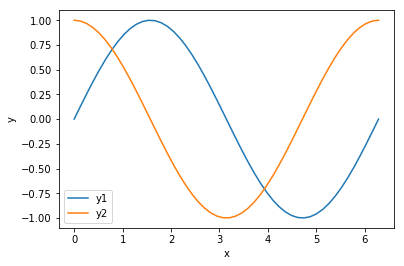
\includegraphics[width=.9\linewidth]{obipy-resources/6316de97116077f6ddc28b130cb204f8-49561f3P.png}
\end{center}

\subsubsection{scipy}
\label{sec:org1cfcf7a}

\href{https://www.scipy.org}{scipy} contains numerous libraries for a broad range of scientific computing needs.

Suppose we want to perform the \href{https://docs.scipy.org/doc/scipy/reference/tutorial/integrate.html\#general-integration-quad}{following integral}: \(I = \int_0^{4.5} J_{2.5}(x) dx\). The function \(J_{2.5}\) is a special function known as a Bessel function. scipy provides both the integration function, and an implementation of the special function we can use.

\begin{minted}[frame=lines,fontsize=\scriptsize,linenos]{ipython}
from scipy.integrate import quad
from scipy.special import jv
\end{minted}

\begin{minted}[frame=lines,fontsize=\scriptsize,linenos]{ipython}
?quad
\end{minted}

\begin{minted}[frame=lines,fontsize=\scriptsize,linenos]{ipython}
?jv
\end{minted}

To evaluate this integral, we have to define a function for the integrand, and use the quad function to compute the integral. The quad function returns two values, the value of the integral, and an estimate of the maximum error in the integral.

\begin{minted}[frame=lines,fontsize=\scriptsize,linenos]{ipython}
# This is how we define a function. There is a function name, and arguments
# The function returns the output of the jv function.
def integrand(x):
    return jv(2.5, x)

I, err = quad(integrand, 0, 4.5)

I, err
\end{minted}

\begin{verbatim}
(1.1178179380783253, 7.866317216380692e-09)
\end{verbatim}

\subsection{Summary}
\label{sec:org7566d01}

Today we introduced several ideas about using Jupyter notebooks to run Python computations. The main points are:

\begin{enumerate}
\item Code is run in code cells
\item You have to import some functions from libraries
\item numpy, scipy and matplotlib are three of the main scientific programming libraries we will use a lot.
\item We saw some ways to get help on functions
\end{enumerate}

Next time we will dig into defining functions more deeply, and how to print formatted strings containing results.

\subsection{Followup actions}
\label{sec:org3878a1c}

By Wednesday, you should all have Anaconda Python 3.6 installed, with techela running.
\section{01 Jupyter}
\label{sec:org3b30249}

Goals today:
\begin{itemize}
\item Explore Jupyter
\item Practice some Markdown
\item Practice making and using functions
\item Practice printing formatted strings
\end{itemize}

\subsection{Markdown}
\label{sec:org1963a78}

Double click on this cell to see how to make:
\begin{enumerate}
\item A
\item Numbered
\item List
\end{enumerate}

You can also make bulleted lists:

\begin{itemize}
\item A
\item bulleted
\item list
\begin{itemize}
\item Including
\begin{itemize}
\item different
\item levels
\end{itemize}
\end{itemize}
\end{itemize}

Text that is \textbf{bold}, \emph{italics}, \sout{crossed-out}. Some <font color="red">red text</font>.

Math is written in \LaTeX{} format (\url{https://en.wikibooks.org/wiki/LaTeX/Mathematics}). Consider:
\begin{itemize}
\item this fraction \(\frac{1}{2}\),
\item square root \(\sqrt{3}\)
\item sum \(\sum_{i=1}^{10} t_i\)
\item A chemical formula: H\$\_2\$O
\item An integral \(\int_a^b f(x)dx\)
\end{itemize}

\noindent\rule{\textwidth}{0.5pt}

You can see more details at \url{https://jupyter-notebook.readthedocs.io/en/stable/examples/Notebook/Working\%20With\%20Markdown\%20Cells.html}.

\noindent\rule{\textwidth}{0.5pt}

You do not need to learn all of these right now. It will be useful to pay attention to what is in the notes. It will help you express your ideas more clearly.

You can convert a cell to Markdown by pressing escape then m. You can convert it back to a Code cell by typing escape then y.

\subsubsection{Headings and subheadings}
\label{sec:org5225518}

It can be helpful to organize your notebook into sections. You can use headings and subheadings to make logical sections.

\begin{enumerate}
\item Subsubheadings
\label{sec:orgfd0c640}

You can learn more about Markdown syntax at \url{https://jupyter-notebook.readthedocs.io/en/stable/examples/Notebook/Working\%20With\%20Markdown\%20Cells.html}.
\end{enumerate}

\subsubsection{Keyboard shortcuts}
\label{sec:org01e4427}

You can do most things by clicking in cells and typing, or clicking on the menus. Eventually, you may want to learn some keyboard shortcuts to speed up your work.

<div class="alert alert-warning">
You can access a list of keyboard shortcuts in the following ways:

\begin{enumerate}
\item Click on the keyboard icon
\item Windows/Linux: Type C-shift-p
\item Mac: Type Cmd-shift-p
\end{enumerate}

From the menus:
Help -> Keyboard Shortcuts
</div>

You do not need to learn these if you don't want to; you can always use the mouse and menus.

\subsection{Running code}
\label{sec:orge552e31}

Jupyter notebooks serve two purposes:

\begin{enumerate}
\item To document your work
\item To run code
\end{enumerate}

It is important to have a basic understanding of how the notebooks work. The browser displays the notebook. The actual computations are run on a server on your computer. When you "run" a code cell, the code is sent to the server, and the server sends the results back to the browser where they are rendered.

When you first open a notebook, \emph{nothing} has been executed. If you try to execute cells out of order, you will get errors if anything in the cell depends on a previous cell. You should run the cells in order. Here are some ways to do that.

\begin{enumerate}
\item Starting in the first cell, click the Run button until you get to the end.
\item Starting in the first cell, click in the menu: Cell -> Run all
\item Starting in the first cell, type shift-Enter to run each cell and move to the next one.
\end{enumerate}

Occasionally, you may want to restart the server and rerun all the cells. Select the menu: Kernel -> Restart \& Run all. If you run cells out of order, or something seems messed up for some reason, sometimes this fixes it. It also makes sure the output of each cell is consistent with running them in order from scratch.

\subsubsection{Debugging/getting help}
\label{sec:org01ec868}

See the Help menu to access general documentation about the notebook and the main libraries we will be using. I would get familiar with their contents, but I would not try to read them all at once.

You should be able to press Shift-tab after a command to get some documentation about the command.

\begin{minted}[frame=lines,fontsize=\scriptsize,linenos]{ipython}
print
\end{minted}

While debugging a cell, you should use C-Enter to run the cell so that you see the output, but your cursor stays in the cell so you can continue editing it. To go back to editing the cell, just press Enter. It is good practice to run cells whenever you think they should work correctly, because it is easier to debug the last few lines you wrote than a long block of lines. Let's work an example.

Create a code cell that defines two variables \(x=5\) and \(y=4\), and then compute \(x^2 + y^2\).

When you are happy with the cell and its output, you can insert a new cell above or below it from the Insert menu or by typing:

\begin{description}
\item[{Esc a enter}] insert a cell above and start editing it
\item[{Esc b enter}] insert a cell below and start editing it
\end{description}

Alternatively, in the cell, type shift-enter to execute it one more time, and then move to the next cell (adds a new cell if you are at the end).

Jupyter notebooks can act in unexpected ways if you evaluate the cells out of order. It can be very difficult to debug this. When that happens, you are often best off if you restart the kernel and execute the cells from the beginning.

\begin{minted}[frame=lines,fontsize=\scriptsize,linenos]{ipython}
a = 4
\end{minted}


\begin{minted}[frame=lines,fontsize=\scriptsize,linenos]{ipython}
a += 1  # this increments the value of a by one.
\end{minted}


\begin{minted}[frame=lines,fontsize=\scriptsize,linenos]{ipython}
print(a)
\end{minted}

\subsection{Functions}
\label{sec:org1661fc5}

Functions are an important part of any programming language. They allow you to reuse code, and make programs more readable.

\subsubsection{Minimal definition of a function with one input}
\label{sec:org23c5abe}

Functions are defined with the \texttt{def} keyword. You specify a name, and the arguments in parentheses, and end the line with a colon. The body of the function must be indented (conventionally by 4 spaces). The function ends when the indentation goes back down one level. You have to define what is returned from the function using the \texttt{return} keyword.

Here is a minimal function definition that simply multiplies the input by two and returns it.

\begin{minted}[frame=lines,fontsize=\scriptsize,linenos]{ipython}
def f(x):
    y = x * 2
    return y
\end{minted}

Let's evaluate our function with a few values:

\begin{minted}[frame=lines,fontsize=\scriptsize,linenos]{ipython}
# Try an integer, float, string, a list, an array (don't forget to import numpy first)
\end{minted}

Python uses "duck-typing" to figure out what multiply by two means. That can lead to some surprising results when you use data types that were not intended for your function.

Minimal is not always the most informative. You can add an optional documentation string like this.

\begin{minted}[frame=lines,fontsize=\scriptsize,linenos]{ipython}
def f(x):
    """Optional, multiline documentation string
    x should be a number. It is still not an error to use a string or array.
    """
    y = x + 2
    return y
\end{minted}

The input argument \texttt{x} is mandatory here, and has no default value.

\subsubsection{Functions with multiple arguments}
\label{sec:org45873d1}

Suppose you want a function where you can multiply the argument by a user-specified value, that defaults to 2. We can define a function with two arguments, where one is optional with a default value. The optional argument is sometimes called a parameter.

\begin{minted}[frame=lines,fontsize=\scriptsize,linenos]{ipython}
def f(x, a=2):
    # The next string is a one line documentation string. The comment here will
    # not be visible in the help.
    "Return a * x. a is optional with default value of 2."
    y = x * a
    return y
\end{minted}

Now, there are several ways to evaluate this function. If you just provide the value of \texttt{x}, then the default value of \texttt{a} will be used.

\begin{minted}[frame=lines,fontsize=\scriptsize,linenos]{ipython}
f(2)  # x = 2, since a is not provided, the default a=2 is used
\end{minted}

\begin{verbatim}
4
\end{verbatim}

Here we use the position of each argument to define the arguments as x=2 and a=3.

\begin{minted}[frame=lines,fontsize=\scriptsize,linenos]{ipython}
f(2, 3) # x=2, a=3
\end{minted}

\begin{verbatim}
6
\end{verbatim}

We can be very clear about the second value by defining it as a keyword argument:

\begin{minted}[frame=lines,fontsize=\scriptsize,linenos]{ipython}
f(2, a=4)
\end{minted}

\begin{verbatim}
8
\end{verbatim}

Note, however, that since the first argument has no default value, it is called a positional argument, and so in this case you must \emph{always} define the first argument as the value of x. This will be an error:

\begin{minted}[frame=lines,fontsize=\scriptsize,linenos]{ipython}
f(a=4, 2)
\end{minted}

\begin{verbatim}
  File "<ipython-input-9-41d646a608d0>", line 1
    f(a=4, 2)
          ^
SyntaxError: positional argument follows keyword argument

\end{verbatim}

You cannot put positional arguments after keyword arguments. This is ok, since every argument is defined by a keyword. This allows you to specify arguments in the order you want, and when there are lots of arguments makes it easier to remember what each one is for.

\begin{minted}[frame=lines,fontsize=\scriptsize,linenos]{ipython}
f(a=4, x=2)
\end{minted}

\begin{verbatim}
8
\end{verbatim}

You should be careful about when and where you define variables. In most programming languages, there is a concept of \emph{variable scope}, that is where is the variable defined, and what value does it have there. Here, \texttt{a} is defined outside the function, so the function inherits the value of \texttt{a} when it is defined. If you change \texttt{a}, you change the function. That can be confusing.

\begin{minted}[frame=lines,fontsize=\scriptsize,linenos]{ipython}
a = 2

def f(x):
    y = a * x
    return y

f(2)
\end{minted}

\begin{verbatim}
4
\end{verbatim}

\begin{minted}[frame=lines,fontsize=\scriptsize,linenos]{ipython}
a = 3  # changing the global value of a changes the function.
f(2)
\end{minted}

\begin{verbatim}
6
\end{verbatim}

However, you can "shadow" a variable. In this example, we use an internal definition of \texttt{a} in the function, which replaces the external value of \texttt{a} \emph{only inside the function}.

\begin{minted}[frame=lines,fontsize=\scriptsize,linenos]{ipython}
a = 2

def f(x):
    a = 3  # This only changes a inside the function
    y = a * x
    return y

f(2)
\end{minted}

\begin{verbatim}
6
\end{verbatim}

The global value of \texttt{a} is unchanged.

\begin{minted}[frame=lines,fontsize=\scriptsize,linenos]{ipython}
a
\end{minted}

\begin{verbatim}
2
\end{verbatim}

A similar behavior is observed with arguments. Here the argument \texttt{a} will shadow (redefine) the global value of \texttt{a}, but only inside the function.

\begin{minted}[frame=lines,fontsize=\scriptsize,linenos]{ipython}
def f(x, a):
    y = a * x
    return y

f(2, a=3)
\end{minted}

\begin{verbatim}
6
\end{verbatim}

The external value of \texttt{a} is unchanged in this case.

\begin{minted}[frame=lines,fontsize=\scriptsize,linenos]{ipython}
a
\end{minted}

\begin{verbatim}
2
\end{verbatim}

The point here is to be careful with how you define and reuse variable names. In this example, it is more clear that we are using an internal definition of \texttt{a}, simply by prefixing the variable name with an underscore (you can also just give it another name, e.g. \texttt{b}).

\begin{minted}[frame=lines,fontsize=\scriptsize,linenos]{ipython}
a = 2

def f(x, _a):
    y = _a * x
    return y

f(2, a=3)
\end{minted}

\subsubsection{Functions that return multiple values}
\label{sec:orgb4b9409}

A function can return multiple values.

\begin{minted}[frame=lines,fontsize=\scriptsize,linenos]{ipython}
def f(x):
    even = x % 2 == 0
    return x, even  # This returns a tuple
\end{minted}

\begin{minted}[frame=lines,fontsize=\scriptsize,linenos]{ipython}
f(2)
\end{minted}

\begin{verbatim}
(2, True)
\end{verbatim}

\begin{minted}[frame=lines,fontsize=\scriptsize,linenos]{ipython}
type(f(2))
\end{minted}

\begin{verbatim}
tuple
\end{verbatim}


\begin{minted}[frame=lines,fontsize=\scriptsize,linenos]{ipython}
f(3)
\end{minted}

\begin{verbatim}
(3, False)
\end{verbatim}

If you assign the output of the function to a variable, it will be a tuple.

\begin{minted}[frame=lines,fontsize=\scriptsize,linenos]{ipython}
z = f(3)
z
\end{minted}

\begin{verbatim}
(3, False)
\end{verbatim}

You can access the elements of the tuple by indexing.

\begin{minted}[frame=lines,fontsize=\scriptsize,linenos]{ipython}
print(z[0])
print(z[1])
\end{minted}

\begin{verbatim}
3
False

\end{verbatim}

You can also \emph{unpack} the tuple into variable names. Here there are two elements in the output, and we can assign them to two variable names.

\begin{minted}[frame=lines,fontsize=\scriptsize,linenos]{ipython}
value, even = f(3)
print(value)
print(even)
\end{minted}

\begin{verbatim}
3
False

\end{verbatim}

You can have the function return any kind of data type. If you just use comma-separated return values, you will return a tuple. If you put them in square brackets, you will return a list. In some cases you will want to return an array. When you write functions, you have to decide what they return, and then use them accordingly. When you use functions that others have written (e.g. from a library), you have to read the documentation to see what arguments are required, and what the function returns.

\subsection{Strings}
\label{sec:org5889624}

We will use strings a lot to present the output of our work. Suppose Amy has 10 apples, and she gives Bob 3 apples. How many apples does Amy have left?

You could solve it like this:

\begin{minted}[frame=lines,fontsize=\scriptsize,linenos]{ipython}
print('Amy has', 10 - 3, 'apples left')
\end{minted}

\begin{verbatim}
Amy has 7 apples left

\end{verbatim}

Or, this more clear code.

\begin{minted}[frame=lines,fontsize=\scriptsize,linenos]{ipython}
original_count = 10
count_given = 3
apples_remaining = original_count - count_given
print(f'Amy has {apples_remaining} apples left.')
\end{minted}

\begin{verbatim}
Amy has 7 apples left.

\end{verbatim}

We have used a \emph{formatted string} here. A formatted string looks like f'\ldots{}', and it has elements inside it in curly brackets that are replaced with values from the environment. We can format the values using formatting codes.

The most common use will be formatting floats. If you just print these, you will get a lot of decimal places, more than is commonly needed for engineering problems.

\begin{minted}[frame=lines,fontsize=\scriptsize,linenos]{ipython}
a = 2 / 3
print(a)
\end{minted}

\begin{verbatim}
0.6666666666666666

\end{verbatim}

We can print this as a float with only three decimal places like this:

\begin{minted}[frame=lines,fontsize=\scriptsize,linenos]{ipython}
print(f'a = {a:1.3f}.')
\end{minted}

\begin{verbatim}
a = 0.667.

\end{verbatim}

The syntax here for float numbers is \{varname:width.decimalsf\}. We will usually set the width to 1, and just change the number of decimal places.

There are other ways to format strings in Python, but I will try to only use this method. It is the most readable in my opinion (note: this only works in Python 3. For Python 2, you may have to use one of the other methods.).

You can do some math inside these strings

\begin{minted}[frame=lines,fontsize=\scriptsize,linenos]{ipython}
volume = 10.0  # L
flowrate = 4.0  # L/s

print(f'The residence time is {volume / flowrate:1.2f} seconds.')
\end{minted}

\begin{verbatim}
The residence time is 2.50 seconds.

\end{verbatim}

You can also call functions in the formatted strings:

\begin{minted}[frame=lines,fontsize=\scriptsize,linenos]{ipython}
def f(x):
    return 1 / x

print(f'The value of 1 / 4.1 to 4 decimal places is {f(4.1):1.4f}.')
\end{minted}

\begin{verbatim}
The value of 1 / 4.1 to 4 decimal places is 0.2439.

\end{verbatim}

There are many ways to use these, and you should use the method that is most readable.

We will see many examples of this in the class. For complete reference on the formatting codes see \url{https://docs.python.org/3.6/library/string.html\#format-specification-mini-language}.

\subsubsection{Printing arrays}
\label{sec:orgfc7a496}

Arrays are printed in full accuracy by default. This often results in hard to read outputs. Consider this array.

\begin{minted}[frame=lines,fontsize=\scriptsize,linenos]{ipython}
import numpy as np

x = np.linspace(0, 10, 4) + 1e-15
x
\end{minted}

\begin{verbatim}
array([  1.000e-15,   3.333e+00,   6.667e+00,   1.000e+01])
\end{verbatim}

You cannot use formatted strings on arrays like this:

\begin{minted}[frame=lines,fontsize=\scriptsize,linenos]{ipython}
print(f'x = {x:1.3f}')
\end{minted}

\begin{verbatim}

TypeErrorTraceback (most recent call last)
<ipython-input-66-42ea60810d4c> in <module>()
----> 1 print(f'x = {x:1.3f}')

TypeError: unsupported format string passed to numpy.ndarray.__format__
\end{verbatim}

You can use this to print individual elements of the array (you access them with [] indexing). First, we print the first element as a float:

\begin{minted}[frame=lines,fontsize=\scriptsize,linenos]{ipython}
print(f'x = {x[0]:1.3f}')
\end{minted}

\begin{verbatim}
x = 0.000

\end{verbatim}

And in exponential (Scientific notation):

\begin{minted}[frame=lines,fontsize=\scriptsize,linenos]{ipython}
print(f'x = {x[0]:1.3e}')
\end{minted}

\begin{verbatim}
x = 1.000e-15

\end{verbatim}


Instead, you can control how arrays are \emph{printed} with this line. Note this does not affect the value of the arrays, just how they are printed. The precision argument specifies how many decimal places, and suppress means do not print very small numbers, e.g. 1e-15 is approximately zero, so print it as zero.

\begin{minted}[frame=lines,fontsize=\scriptsize,linenos]{ipython}
np.set_printoptions(precision=3, suppress=True)
x
\end{minted}

\begin{verbatim}
array([  0.   ,   3.333,   6.667,  10.   ])
\end{verbatim}

Here we just illustrate that x[0] is not zero as printed. If it was, we would get a DivisionByZero error here.

\begin{minted}[frame=lines,fontsize=\scriptsize,linenos]{ipython}
1 / x[0]
\end{minted}

\begin{verbatim}
999999999999999.88
\end{verbatim}
\subsection{Summary}
\label{sec:org1b68195}

You should get comfortable with:
\begin{itemize}
\item Creating markdown cells in Jupyter notebooks that express the problem you are solving, and your approach to it.
\item Creating code cells to evaluate Python expressions
\item Defining functions with arguments
\item Printing formatted strings containing your results
\end{itemize}

Next time:
We will start using functions to solve integrals and differential equations.

\section{02 Introduction to integration}
\label{sec:orgf66b756}
Integration is used for many purposes in scientific problem solving. It can:

\begin{enumerate}
\item Represent the area under a curve or between curves
\item Solve differential equations
\end{enumerate}

We may have data that represents a function that needs to be integrated, or a function we want to integrate, or a differential equation we want to solve. We may also have data that represents a some function, and that we wish to integrate.

Historically, we would have to look up or remember the formula for an integral, e.g. in a book like this (16\(^{\text{th}}\) ed. CRC Standard Mathematical Tables):

\url{\~/Downloads/IMG\_1889.JPG}

There are a limited number of known analytical integrals, and for everything else, we have to resort to numerical/computational approaches to evaluate them.



\subsection{Numerical integration of data}
\label{sec:org7cb1cff}

Data can be used to represent functions. Suppose we have the function \(y=x^2\), and 5 \(x\) values evenly spaced from 0 to 4. We can represent this function numerically with data like this.

\begin{minted}[frame=lines,fontsize=\scriptsize,linenos]{ipython}
import numpy as np

x = np.linspace(1, 4, 5)
y = x**2

%matplotlib inline
import matplotlib.pyplot as plt

plt.plot(x, y, 'bo--')  # plot with blue circles connected by a dashed line
plt.xlabel('x')
plt.ylabel('y')
\end{minted}

\begin{center}
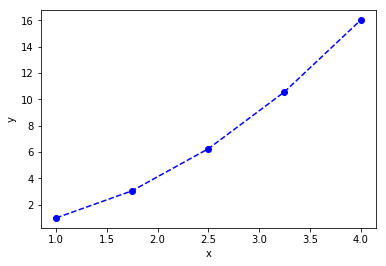
\includegraphics[width=.9\linewidth]{obipy-resources/d9632b07b477acbf48eabd2bf122330e-49561Tnc.png}
\end{center}

If we want the area under this curve, it is represented by:

\(A = \int_0^4 x^2 dx\)

We could analytically evaluate this as:

\(A = \frac{1}{3} (4^3 - 1^3)\).

Here is the analytical answer for future reference:

\begin{minted}[frame=lines,fontsize=\scriptsize,linenos]{ipython}
1 / 3 * (4**3 - 1**3)
\end{minted}

\begin{verbatim}
21.0
\end{verbatim}

It will not always be the case that we can evaluate the integrals analytically, and sometimes we just have the data, and not the analytical function it represents (e.g. if you have measured the data).


The classical way to compute the error under this curve is to use the trapezoid method. We know the area of a trapezoid is \(A = 0.5 * width * (y1 + y2)\). In this example, we have four trapezoids to compute the areas of.

To make this easier to compute, we need a few new ideas. First, it would be convenient to know how many elements are in the array \texttt{x}.

\begin{minted}[frame=lines,fontsize=\scriptsize,linenos]{ipython}
len(x)
\end{minted}

\begin{verbatim}
5
\end{verbatim}

Second, we need to know how to compute the area of a trapezoid defined by the points in \texttt{x} and \texttt{y}. The area of the first trapezoid is defined by:

\begin{minted}[frame=lines,fontsize=\scriptsize,linenos]{ipython}
0.5 * (y[0] + y[1]) * (x[1] - x[0])
\end{minted}

\begin{verbatim}
1.5234375
\end{verbatim}

What we would like to do is to loop over each trapezoid, compute the area, and accumulate it in a variable. Here is how we use a \texttt{for} loop to iterate from a value starting at 1 to the length of the array \texttt{x}. Note that although the length is 5, the last value of \texttt{i} is 4. The loop goes up to, but not including the last value of the range.

\begin{minted}[frame=lines,fontsize=\scriptsize,linenos]{ipython}
for i in range(1, len(x)):
    print(i)
\end{minted}

\begin{verbatim}
1
2
3
4

\end{verbatim}


\begin{minted}[frame=lines,fontsize=\scriptsize,linenos]{ipython}
area = 0.0  # variable we will accumulate the area in

for i in range(1, len(x)):
    y1 = y[i - 1]
    y2 = y[i]
    width = x[i] - x[i - 1]
    area += 0.5 * width * (y1 + y2)  # increment the area variable

print(f'The estimated area is {area}.')
print(f'The exact area is {1 / 3 * (x[-1]**3 - x[0]**3)}')
\end{minted}

\begin{verbatim}
The estimated area is 21.28125.
The exact area is 21.0

\end{verbatim}

Why don't these agree? The trapezoid method is an approximation of the integral. In this case the straight lines connecting the points \emph{overestimate} the value of the function, and so the area under this curve is overestimated.

\textbf{Exercise}: Increase the number of points slowly and see how the estimate converges to the exact value.

\subsubsection{numpy.trapz}
\label{sec:orgc590164}

It is somewhat tedious to write the loop above, making sure you get the indexing right, etc. The trapezoid method is defined in numpy. See the help for how to use it:

\begin{minted}[frame=lines,fontsize=\scriptsize,linenos]{ipython}
?np.trapz
\end{minted}

Now, we can perform the integration with just one line:

\begin{minted}[frame=lines,fontsize=\scriptsize,linenos]{ipython}
import numpy as np
x = np.linspace(1, 4, 5)
y = x**2
np.trapz(y, x)
\end{minted}

\begin{verbatim}
21.28125
\end{verbatim}

The trapezoid method is only exact for lines. For everything else, it is an approximation. For functions (or regions) that are concave up, the trapezoid method will over-estimate the integral, and for regions that are concave down, the method will underestimate the true integral.

The \href{https://en.wikipedia.org/wiki/Trapezoidal\_rule\#Error\_analysis}{error} in this method is formally:

\(error = - \frac{(b - a)^3}{12 N^2} f''(\xi)\)

In this formula, \(\xi\) is some number between \(a\) and \(b\), in other words the error is related to the second derivative of the function evaluated somewhere in the interval.

Practically, we only use this method for integrating data where we do not know the function it represents, so we cannot reliably estimate the error in the integral.

\subsubsection{Simpson method \url{https://docs.scipy.org/doc/scipy-0.18.1/reference/generated/scipy.integrate.simps.html\#scipy.integrate.simps}}
\label{sec:org3cca5bb}

There are more advanced approximations to integration than the trapezoid method. With the trapezoid method, you essentially assume linear interpolation between the points, and in the limit of infinite points that are close together, this is reasonable. We rarely get to that limit however.

Instead of linear interpolation, we can use quadratic interpolation, where one uses the point and its neighbors to compute the equation of a parabola that goes through them, and then analytically computes the area under the parabola over the relevant interval. This is the basis of \href{https://en.wikipedia.org/wiki/Simpson\%27s\_rule}{Simpson's method}. There is an excellent animation of Simpson's Rule at that page.


Note in this case, since we integrate a parabola, the result is exact. It will not be exact in general, but this method is generally expected to be more accurate than the trapezoid method for well-behaved data because it represents the local curvature better than lines do.

\begin{minted}[frame=lines,fontsize=\scriptsize,linenos]{ipython}
from scipy.integrate import simps

simps(y, x)
\end{minted}

\begin{verbatim}
21.0
\end{verbatim}

\subsubsection{Applications}
\label{sec:orgc035342}

\begin{enumerate}
\item Estimating the volume of a solid
\label{sec:org4977fcd}

We can use integrals to compute the volume of solids. If we know how the cross-sectional area of a solid varies in some direction, we simply evaluate the following integral:

\(\int_{x0}^{x1} A(x) dx\)

For a sphere, we can derive:

\(A(x) = \pi (1 - x^2)\)

\begin{minted}[frame=lines,fontsize=\scriptsize,linenos]{ipython}
R = 1
x = np.linspace(-R, R)
y = np.pi * (1 - x**2)

approx_V = np.trapz(y, x)
exact_V = 4 / 3 * np.pi * R**3

print(f'''Approximate volume = {approx_V:1.4f}
Exact volume = {exact_V:1.4f}''')
\end{minted}

\begin{verbatim}
Approximate volume = 4.1870
Exact volume = 4.1888

\end{verbatim}

With 50 points, the estimate is pretty good. Try increasing the number of points to improve the estimate.

\item Estimating the volume of a plug flow reactor
\label{sec:org4c72052}

Adapted from Fogler example 2.7. The volume of a plug flow reactor is defined by this integral:

\(\int_{X0}^{X1} \frac{F_{A0}}{-r_A} dX\)

where \(F_{A0}\) is the inlet molar flow of species A, \(X\) is the conversion, and \(-r_A\) is the rate of generation of species A per unit volume. \(r_A\)  is a function of conversion. We often do not know what the function is, but we can measure the rate of generation. Below is some tabulated data of the rate of generation of species A as a function of conversion.

\begin{center}
\begin{tabular}{rr}
X & -r\_A (kmol / m\^{}3 / hr)\\
\hline
0 & 39\\
0.2 & 53\\
0.4 & 59\\
0.6 & 38\\
0.65 & 25\\
\end{tabular}
\end{center}

Use this data to estimate the volume of the reactor required to achieve a conversion of 0.65.

\begin{minted}[frame=lines,fontsize=\scriptsize,linenos]{ipython}
X = np.array([0, 0.2, 0.4, 0.6, 0.65])

ra = -np.array([39, 53, 59, 38, 25])

Fa0 = 50 # kmol / hr.

V = np.trapz(Fa0 / -ra, X)

print(f'The required volume is {V:1.3f} m^3.')
\end{minted}

\begin{verbatim}
The required volume is 0.701 m^3.

\end{verbatim}

How does the volume depend on conversion? Let's plot the integrand first so we can get a sense for how the area might change with conversion.

\begin{minted}[frame=lines,fontsize=\scriptsize,linenos]{ipython}
plt.plot(X, Fa0 / -ra)
plt.xlabel('Conversion')
plt.ylabel('$F_{A0} / -r_A$')
plt.xlim([0, 0.65])
plt.ylim([0, 2])
\end{minted}

\begin{verbatim}
(0, 2)
\end{verbatim}



\begin{center}
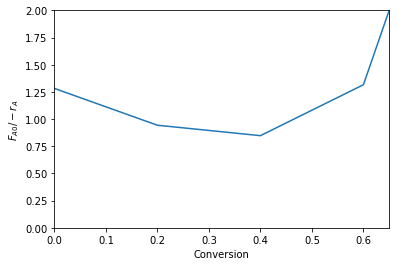
\includegraphics[width=.9\linewidth]{obipy-resources/d9632b07b477acbf48eabd2bf122330e-1814nA.png}
\end{center}

We could iterate over the conversions and print the volume for each value. This is a little wasteful since we recompute the areas in each iteration, but here it is so fast it does not matter.

Before jumping into the integration an loop, Let's review array slicing. It allows us to select portions of arrays for analysis.

\begin{minted}[frame=lines,fontsize=\scriptsize,linenos]{ipython}
# X[start:below_end]
X = np.array([0, 0.2, 0.4, 0.6, 0.65])
X[0:3] # This selects points with indices 0-2
\end{minted}

\begin{verbatim}
array([ 0. ,  0.2,  0.4])
\end{verbatim}

We use -1 for the last element (-2 for second to last element, etc). Note that this \emph{does not} include the last element.

\begin{minted}[frame=lines,fontsize=\scriptsize,linenos]{ipython}
X[1:-1]
\end{minted}

\begin{verbatim}
array([ 0.2,  0.4,  0.6])
\end{verbatim}

To get to the last element, we do not specify an end value like this:

\begin{minted}[frame=lines,fontsize=\scriptsize,linenos]{ipython}
X[1:]
\end{minted}

\begin{verbatim}
array([ 0.2 ,  0.4 ,  0.6 ,  0.65])
\end{verbatim}

So, back to the integration. We need to use slices of the array for each integration step.

\begin{minted}[frame=lines,fontsize=\scriptsize,linenos]{ipython}
y = Fa0 / -ra

volumes = []  # empty list to store values in

for i in range(0, len(X)):
    vol = np.trapz(y[0:i+1], X[0:i+1])
    volumes += [vol] # here we accumulate the vol into our list
    print(f'At X={X[i]:3.2f} V={vol:1.3f} m^3')

volumes
\end{minted}

\begin{verbatim}
At X=0.00 V=0.000 m^3
At X=0.20 V=0.223 m^3
At X=0.40 V=0.402 m^3
At X=0.60 V=0.618 m^3
At X=0.65 V=0.701 m^3

\end{verbatim}

\begin{verbatim}
[0.0,
 0.22254475084663766,
 0.40163013620001153,
 0.61795484628029695,
 0.70084958312240231]
\end{verbatim}

An alternative approach is to use a cumulative trapezoid function. This is defined in scipy.integrate. The main benefit of this approach is that it is faster, as it does not recompute the areas, and the code is shorter, so there are less places to make mistakes!

\begin{minted}[frame=lines,fontsize=\scriptsize,linenos]{ipython}
import scipy as sp
cumV = sp.integrate.cumtrapz(Fa0 / -ra, X)

plt.plot(X[1:], cumV)
plt.xlabel('Conversion')
plt.ylabel('Volume (m$^3$)')

cumV
\end{minted}

\begin{verbatim}
array([ 0.22254475,  0.40163014,  0.61795485,  0.70084958])
\end{verbatim}



\begin{center}
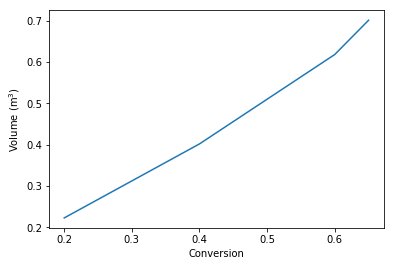
\includegraphics[width=.9\linewidth]{obipy-resources/d9632b07b477acbf48eabd2bf122330e-181FyG.png}
\end{center}

What if you want to know the volume required for an intermediate conversion? For that you need interpolation. We will cover that later in the course when we talk more about dealing with data.
\end{enumerate}


\subsection{Numerical quadrature}
\label{sec:orgd410364}

When you have a function and you know its analytical form we can use quadrature to estimate integrals of it. In quadrature, we approximate the integral as a weighted sum of function values. By increasing the number values used, we can systematically improve the integral estimates.

To motivate the idea, let's consider the function integral of \(y(x) = 7 x^3 - 8 x^2 - 3x +3\) from -1 to 1.

This is a third order polynomial, so we can in this case replace the integral with a sum of two points:

\(\int f(x) dx = w_1 f(x_1) + w_2 f(x_2)\)

provided we can find the weights, and the right values of \(x\) to use. These are derived and tabulated (e.g. at \url{https://en.wikipedia.org/wiki/Gaussian\_quadrature}), which tells us for this case, the weights are simply equal to one, and we should use \(\pm \sqrt{1/3}\) for x.

\begin{minted}[frame=lines,fontsize=\scriptsize,linenos]{ipython}
%matplotlib inline
import matplotlib.pyplot as plt

x = np.linspace(-1, 1)

def f(x):
    return 7 * x**3 - 8 * x**2 - 3 * x + 3

plt.plot(x, f(x))

f(np.sqrt(1/3)) + f(-np.sqrt(1/3))
\end{minted}

\begin{verbatim}
0.66666666666666741
\end{verbatim}



\begin{center}
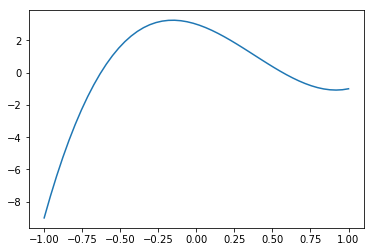
\includegraphics[width=.9\linewidth]{obipy-resources/d9632b07b477acbf48eabd2bf122330e-181BeY.png}
\end{center}

This example is special in several ways:
\begin{enumerate}
\item The formula was derived for n\(^{\text{th}}\) order polynomials, here we had a 3rd order polynomial, so n-1 points are needed to exactly compute the integral. The formula is not exact for non-polynomial functions.
For non-poynomial functions, the formula is an approximation to the integral and you have to use more than two points to estimate the integral. When you use more points, the weights change, but they can be looked up in the table, or computed.
\end{enumerate}

I show this example mostly to motivate the idea that given a function, you can perform an integral by evaluating the function at special points, and weighting those function values appropriately. In practice, we don't do this manually. It has been coded already into robust libraries that we can reuse.

\texttt{scipy.integrate} provides the \href{https://docs.scipy.org/doc/scipy-0.18.1/reference/generated/scipy.integrate.quad.html\#scipy.integrate.quad}{quad} function. This is a Python wrapper around a sophisticated \href{https://en.wikipedia.org/wiki/QUADPACK}{Fortran library} for integrating functions. These routines use an adaptive method to compute the integral and provide an upper bound on the error of the computed integral. The beauty of this interface is we can use a reliable, proven library written in Fortran inside of Python. We do not have to write and compile a Fortran program ourselves.

\begin{minted}[frame=lines,fontsize=\scriptsize,linenos]{ipython}
from scipy.integrate import quad

?quad
\end{minted}

We return to our simple integral, which should equal 21.

\begin{minted}[frame=lines,fontsize=\scriptsize,linenos]{ipython}
4**3 / 3 - 1 / 3  # analytical integral of x^2 from 1 to 4.
\end{minted}

\begin{verbatim}
21.0
\end{verbatim}

To use the quad function, we define a function, and use it as the first argument in the quad function. The quad function returns the integral value, and estimated error.

\begin{minted}[frame=lines,fontsize=\scriptsize,linenos]{ipython}
def f(x):
    return x**2

quad(f, 1, 4)
\end{minted}

\begin{verbatim}
(21.000000000000004, 2.331468351712829e-13)
\end{verbatim}

We can recompute the volume of a sphere much more precisely, and easily now. Recall \(A(x) = \pi (1 - x^2)\) and that \(V = \int_{-1}^{1} A(x) dx\). Here is the implementation.

\begin{minted}[frame=lines,fontsize=\scriptsize,linenos]{ipython}
def cross_section(x):
    return np.pi * (1 - x**2)

quad(cross_section, -1, 1)
\end{minted}

\begin{verbatim}
(4.1887902047863905, 4.6504913306781755e-14)
\end{verbatim}

We can integrate to infinity.

\(\int_{-\infty}^{\infty} \frac{1}{x^2 + 1} = \pi\).

Let us verify this. You can use \textpm{} \(\infty\) as limits.

\begin{minted}[frame=lines,fontsize=\scriptsize,linenos]{ipython}
def f(x):
    return 1 / (x**2 + 1)

quad(f, -np.inf, np.inf)
\end{minted}

\begin{verbatim}
(3.141592653589793, 5.155583041103855e-10)
\end{verbatim}

Not all integrals are finite. For example

\(\int_1^\infty \frac{dx}{x} = \infty\)

Here we get an IntegrationWarning that a maximum number of subdivisions has been achieved.

\begin{minted}[frame=lines,fontsize=\scriptsize,linenos]{ipython}
def f(x):
    return 1 / x

quad(f, 1, np.infty)
\end{minted}

\begin{verbatim}
/Users/jkitchin/anaconda/lib/python3.6/site-packages/scipy/integrate/quadpack.py:364: IntegrationWarning: The maximum number of subdivisions (50) has been achieved.
  If increasing the limit yields no improvement it is advised to analyze
  the integrand in order to determine the difficulties.  If the position of a
  local difficulty can be determined (singularity, discontinuity) one will
  probably gain from splitting up the interval and calling the integrator
  on the subranges.  Perhaps a special-purpose integrator should be used.
  warnings.warn(msg, IntegrationWarning)

\end{verbatim}

\begin{verbatim}
(40.996012819169536, 8.156214940493651)
\end{verbatim}

Math is fun though, this subtly different function is integrable:

\begin{minted}[frame=lines,fontsize=\scriptsize,linenos]{ipython}
def f(x):
    return 1 / x**2

quad(f, 1, np.infty)
\end{minted}

\begin{verbatim}
(1.0, 1.1102230246251565e-14)
\end{verbatim}

And this function is integrable, despite the singularity at x=0.

\begin{minted}[frame=lines,fontsize=\scriptsize,linenos]{ipython}
def f(x):
    return 1 / np.sqrt(x)

quad(f, 0, 1)
\end{minted}

\begin{verbatim}
(1.9999999999999984, 5.773159728050814e-15)
\end{verbatim}

\subsubsection{Find the volume of a PFR}
\label{sec:orgb23aadf}

For a single reaction that consumes a species A at a rate of \(-r_A = k C_A\), a mole balance leads to an equation for the volume as a function of conversion \(X\) as:

\(V = \int_0^X \frac{F_{A0}}{-r_A(X)} dX\)

\(F_{A0}\) is the inlet molar flow of species A, which is equal to the inlet concentration times the inlet volumetric flow. The concentration of A in the reactor is a function of the conversion, and is given by  \(C_A = C_{A0} (1 - X)\). If \(k = 0.23\) 1/min, \(C_{A0} = 1\) mol/L, and the volumetric flow is 1 L/min, what is the reactor volume required to achieve a conversion of 50\%?

\begin{minted}[frame=lines,fontsize=\scriptsize,linenos]{ipython}
from scipy.integrate import quad

k = 0.23
Ca0 = 1.0
v0 = 1.0

Fa0 = v0 * Ca0

def rA(X):
    Ca = Ca0 * (1 - X)
    return -k * Ca

def integrand(X):
    return Fa0 / -rA(X)

vol, err = quad(integrand, 0, 0.5)
print(f'The required volume is {vol:1.3f} L')
\end{minted}

\begin{verbatim}
The required volume is 3.014 L

\end{verbatim}
\subsubsection{Diffusion}
\label{sec:org92ecf54}

When the surface concentration of a solute is constant, and the solute diffused into a semi-infinite solid, the concentration of the solute in the solid varies with space and time according to:
\(C_A(x, t) = C_{As} - (C_{As} - C_{A0}) erf\left(\frac{x}{\sqrt{4 D t}}\right)\).

\(C_{As}\) is the concentration of the diffusing species at \(x=0\), and \(C_{A0}\) is the initial concentration of the species in the semi-infinite body.

and \(erf(x) = \frac{2}{\sqrt{\pi}} \int_0^x e^-{\xi^2} d\xi\)

This integral arises from the solution to the differential equation describing diffusion. The integral does not have an analytical solution, but it can be solved numerically.

Suppose we have a steel sample \#1 that initially contains 0.02\% Carbon in it, and it is put in contact with another steel containing 1.2\% carbon. If the diffusion coefficient of carbon is 1.54e-6 cm\^{}2/s, what will the concentration of carbon in sample \#1 be after 24 hours?

\begin{minted}[frame=lines,fontsize=\scriptsize,linenos]{ipython}
Cas = 1.2
Ca0 = 0.02
D = 1.54e-6 # cm^2/s
X = 0.15 # cm
t = 24 * 60 * 60 # time in seconds


xi = X / np.sqrt(4 * D * t)

def erf_integrand(xi):
    return 2 / np.sqrt(np.pi) * np.exp(-xi**2)

erfx, err = quad(erf_integrand, 0, xi)

Cx = Cas - (Cas - Ca0) * erfx
print(f'The concentration of carbon at X = {X} cm after {t / 3600} hours is {Cx:1.2f}%.')
\end{minted}

\begin{verbatim}
The concentration at X = 0.15 cm after 24.0 hours is 0.93%.

\end{verbatim}

The \href{https://en.wikipedia.org/wiki/Error\_function}{error function}, \(erf(x)\) is such an important function it is implemented as a special function in scipy.special.

\begin{minted}[frame=lines,fontsize=\scriptsize,linenos]{ipython}
from scipy.special import erf

Cx_wspecial = Cas - (Cas - Ca0) * erf(xi)
print(f'The concentration of carbon at X = {X} cm after {t / 3600} hours is {Cx_wspecial:1.2f}%.')
\end{minted}

\begin{verbatim}
The concentration of carbon at X = 0.15 cm after 24.0 hours is 0.93%.

\end{verbatim}


\subsection{Summary}
\label{sec:orgec80eae}

The main points of this lecture were on

\begin{itemize}
\item Numerical integration of data
\begin{itemize}
\item I recommend you rely on library implementations of the trapezoid method or Simpson's method.
\item \texttt{numpy.trapz}, \texttt{scipy.integrate.cumtrapz}, and \texttt{scipy.integrate.simps}.
\end{itemize}

\item Integration of functions by quadrature
\begin{itemize}
\item quadrature uses a weighted sum of function evaluations to estimate the integrals.
\item I recommend you rely on a library implementation of a quadrature
\begin{itemize}
\item e.g. \texttt{scipy.integrate.quad}.
\item These libraries provide sophisticated convergence algorithms and error estimates
\end{itemize}
\end{itemize}
\end{itemize}

Next time we will consider using integration to obtain solutions to differential equations.

\section{03 First-order differential equations}
\label{sec:org39b563c}

\subsection{Solutions to first-order differential equations by integration}
\label{sec:orgb01ec23}

Adapted from Ch. 2 in Advanced Engineering Mathematics, 2\(^{\text{nd}}\) Ed. by Michael Greenberg.

\subsubsection{Homogeneous, first-order linear differential equations}
\label{sec:orgfe3b55c}

We first consider a homogeneous, first-order, linear differential equation of the form:

\(y' + p(x) y = 0\), with \(y(a) = b\) as an initial value.

You can derive a solution to this ODE as:

\(y(x) = b e^{-\int_a^x p(\xi) d\xi}\)

For concreteness, consider \((x+2) y' - xy = 0, y(0) = 3\)

what is the value of \(y(1)\)?

We need to cast this in the form required to identify \(p(x)\). That form is:

\(y' + \frac{-x}{x+2}y = 0\).

Now, we simply evaluate the required integral and use it to compute the value of the solution at the desired new \(x\) value.

\begin{minted}[frame=lines,fontsize=\scriptsize,linenos]{ipython}
a = 0
b = 3
x1 = 1

def p(x):
    return -x / (x + 2)

import numpy as np
from scipy.integrate import quad

I, err = quad(p, a, x1)

y_x1 = b * np.exp(-I)

print(f'y(1) = {y_x1:1.3f}')
\end{minted}

\begin{verbatim}
y(1) = 3.624

\end{verbatim}

It is a little trickier to evaluate the solution at several x-values, e.g. to make a plot. The \texttt{quad} function is not "vectorized", meaning it only performs one integral for one range at a time. You cannot pass it a list of ranges to evaluate it several times. Instead, we have to use a loop for this. In the loop, we will solve the integral, and accumulate the result in a solution array. Before we do that, here are a few useful commands we will need to use.

First, it is useful to make an array to store the results in. There are a few ways to do this, the one we use today is the \texttt{np.zeros} function. You specify the size of the array as an argument. For example, to make an array with three zeros, do this:

\begin{minted}[frame=lines,fontsize=\scriptsize,linenos]{ipython}
np.zeros(3)
\end{minted}

\begin{verbatim}
array([ 0.,  0.,  0.])
\end{verbatim}

Second, it is helpful to get the shape of an array. You use dot notation and the shape attribute of an array for this. This allows you to create an array, and later make an array of zeros with the same shape and size.

\begin{minted}[frame=lines,fontsize=\scriptsize,linenos]{ipython}
x = np.linspace(0, 3.5)
x.shape
\end{minted}

\begin{verbatim}
(50,)
\end{verbatim}

Finally we will iterate over the elements of the x array, and in each step we need to know the index of the element \emph{and} the value of the element. \texttt{enumerate} provides this in a pretty straightforward syntax. This function iterates over an array and returns at each step the index and element, which you can assign to variables that you use inside the loop. There are other ways to achieve this, but we only consider this method today. Here, we create an array, and an array of zeros that is the same shape. Then, we iterate over the first array, and set the corresponding index in the second array equal to a computation using the index and element value.

\begin{minted}[frame=lines,fontsize=\scriptsize,linenos]{ipython}
arr = np.linspace(0, 1, 5)
new_arr = np.zeros(arr.shape)
print(f'Before the loop new_arr = {new_arr}')

for i, val in enumerate(arr):
    new_arr[i] = i * val
    print(f'The element at index {i} is {val}')

print(f'After the loop new_arr = {new_arr}')
\end{minted}

\begin{verbatim}
Before the loop new_arr = [ 0.  0.  0.  0.  0.]
The element at index 0 is 0.0
The element at index 1 is 0.25
The element at index 2 is 0.5
The element at index 3 is 0.75
The element at index 4 is 1.0
After the loop new_arr = [ 0.    0.25  1.    2.25  4.  ]

\end{verbatim}

Back to the solution to our integration problem. Our goal is to compute the value of the solution for an array of x-values. We will iterate over an array of x-values, and for each one compute the value of the solution at that x, and save the solution in a new array.

\begin{minted}[frame=lines,fontsize=\scriptsize,linenos]{ipython}
x = np.linspace(0, 3.5)
y = np.zeros(x.shape)

for i, x1 in enumerate(x):
    I, err = quad(p, a, x1)
    y[i] = b * np.exp(-I)

%matplotlib inline
import matplotlib.pyplot as plt
plt.plot(x, y)
plt.xlabel('x')
plt.ylabel('y')
plt.xlim([x.min(), x.max()])
\end{minted}

\begin{verbatim}
(0.0, 3.5)
\end{verbatim}



\begin{center}
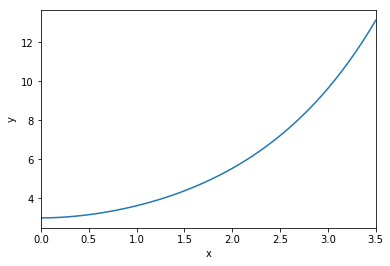
\includegraphics[width=.9\linewidth]{obipy-resources/744bcb3e58866fd0750c7a1efd9d42e8-68311qjJ.png}
\end{center}

We should ask, how can we tell this is correct? We can confirm the initial values, which we know are correct.

\begin{minted}[frame=lines,fontsize=\scriptsize,linenos]{ipython}
x[0], y[0]
\end{minted}

\begin{verbatim}
(0.0, 3.0)
\end{verbatim}

We can express the ODE as: \(y' = \frac{x}{x+2}y\). By inspection, we can see that the derivative will always be positive, so the solution should increase from the initial value, which it does.

We can also examine the derivatives of our solution. We have to rely on numerical derivatives of our solution because x and y are arrays. \texttt{np.gradient} will compute the derivative using a reasonable approximation. We know the derivative analytically from the ODE.

\begin{minted}[frame=lines,fontsize=\scriptsize,linenos]{ipython}
dydx = np.gradient(y, x)

plt.plot(x, dydx, label='numerical')
plt.plot(x, x / (x + 2) * y, 'r--', label='analytical')
plt.xlabel('x')
plt.ylabel('dy/dx')
plt.legend()
\end{minted}

\begin{center}
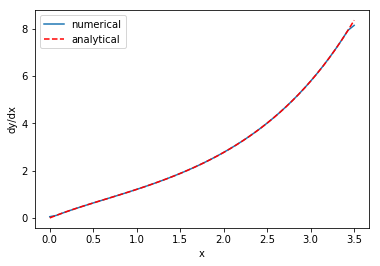
\includegraphics[width=.9\linewidth]{obipy-resources/744bcb3e58866fd0750c7a1efd9d42e8-683113tP.png}
\end{center}

Here you see good agreement over most of the range. The end-points are always less accurate because the derivatives there are approximated by a less accurate formula. We interpret the sum of this evidence to mean our solution to the ODE is good over this range of x values.

\subsubsection{Non-homogeneous linear first-order ODEs}
\label{sec:org3691c6a}

A non-homogenous first order, linear differential equation has this form:

\(y' + p(x) y = q(x), y(a)=b\)

Equations of this form are typically solved with a method called variation of parameters. In the most general form, this leads to solutions of the form:

\(y(x) = e^{-\int_a^x p(\xi)d\xi}\left(\int_a^x e^{-\int_a^{\xi} p(\zeta)d\zeta} q(\xi)d\xi + b\right)\)

It is a little tricky to implement this. It is helpful to break this down into several pieces. Note that it is not necessary to do this, it just makes it easier to read, debug, and see that you have done it correctly. Here are the easiest parts.

\begin{minted}[frame=lines,fontsize=\scriptsize,linenos]{ipython}
def p(xi):
    return -2 * xi

def q(xi):
    return np.sin(xi)

a = 0
b = 3
\end{minted}

Next, we will break the equation into two parts:

\(y(x) = term1 * term2\) where

\(term1 = e^{-\int_a^x p(\xi)d\xi}\)

and

\(term2 = \left(\int_a^x e^{-\int_a^{\xi} p(\zeta)d\zeta} q(\xi)d\xi + b\right)\)

We can immediately define a function for term1 as:

\begin{minted}[frame=lines,fontsize=\scriptsize,linenos]{ipython}
def term1(x):
    I1, _ = quad(p, a, x)
    return np.exp(-I1)
\end{minted}

term2 is a little trickier, as it has a partial integral inside an integral. We can define a function for this term also, but we have to define an internal function to use for the integral. The internal function will have an integral inside of it.

\begin{minted}[frame=lines,fontsize=\scriptsize,linenos]{ipython}
def term2(x):

    def integrand(xi):
        internal_term1, _ = quad(p, a, xi)
        internal_term2 = q(xi)
        return np.exp(internal_term1) * internal_term2

    I2, _ = quad(integrand, a, x)
    return I2 + b
\end{minted}

Now, to use it, we form the product of the two terms:

\begin{minted}[frame=lines,fontsize=\scriptsize,linenos]{ipython}
x1 = 0.5
print(term1(x1) * term2(x1))
\end{minted}

\begin{verbatim}
3.99127653383

\end{verbatim}

With some algebra and calculus on your part, you might arrive at the following non-elementary integral solution:

\(y(x) = e^{x^2} \left(\int_0^x e^{-\xi^2} \sin{\xi} d\xi + 3\right)\)

The solution is called non-elementary because you cannot evaluate the integral in closed form using elementary functions, e.g. powers of x, trigonometric functions, exponentials or logarithms. You can, however, use numerical methods to integrate it.

\begin{minted}[frame=lines,fontsize=\scriptsize,linenos]{ipython}
def integrand(x):
    return np.exp(-x**2) * np.sin(x)

I, _ = quad(integrand, 0, x1)

sol = np.exp(x1**2) * (I + b)
sol
\end{minted}

\begin{verbatim}
3.9912765338345242
\end{verbatim}

Note there is some conservation of effort here. If you can derive the solution above correctly (and you have all learned how to do this if you had a differential equations course), the code below is quite short to get the solution at some value of x. If you are unable to derive that solution, you can use the general solution we gave, but then it is a trickier solution to implement in code.

\subsubsection{Limitations of solutions by integration}
\label{sec:orgc9ed77d}

Solution by integration has some advantages. You get an estimate of the error in the solution from the \texttt{quad} function, which is helpful to know how good the solution is. However, the methods described above are limited to \emph{linear} differential equations of the form described. If you have a nonlinear differential equation, or if you are unable to separate the equations into integrable form, the methods simply don't work. Next, we consider how to approach equations where we cannot use integration to solve the problems.

\subsection{Numerical solutions to differential equations}
\label{sec:orgee329e9}

We begin with a brief review of first order differential equations. The equations we are concerned with here all have the form:

\(\frac{dy}{dx} = f(x, y)\)

And the value of the solution is known at some point, e.g. \(y(x0) = y0\). \(f(x, y)\) can be linear or nonlinear. Our goal in this section is to motivate how numerical solutions are obtained.

These notes were adapted from Chapter 6 in Advanced Engineering Mathematics 2\(^{\text{nd}}\) ed. by Michael D. Greenberg.

The basic idea behind these methods is that we know the initial value of the solution \emph{and} the derivative of the solution (it is defined by the ODE definition above), and so we can estimate the solution a small distance away from the initial value. If you repeat this process with the newly estimated point, you can estimate the next point, and so on. There are many algorithms for performing the estimation, and we will consider a two of them. These algorithms differ in efficiency, ease of implementation, and accuracy.

\subsubsection{Euler's method}
\label{sec:org30398dc}

The main idea of Euler's method is that if you know the value of the solution at some point, and you know the derivative at that point, you can estimate the solution nearby at \(x0 + h\), where \(h\) is a small number:

\(y_{n+1} = y_n + f(x_n, y_n) h\)

Now, you just repeat this until you get to the x-value that you want. For concreteness, consider:

\(y' = y + 2x - x^2; y(0) = 1\).

This ODE has a known analytical solution: \(y(x) = x^2 + e^x\). We will use this for comparison.

\begin{minted}[frame=lines,fontsize=\scriptsize,linenos]{ipython}
import numpy as np

def f(x, y):
    return y + 2 * x - x**2

x0 = 0
y0 = 1

x, h = np.linspace(x0, 1.5, 5, retstep=True)  # Note the optional argument to get the stepsize.
print(f'h = {h}')

y = np.zeros(x.shape)
y[0] = y0

# Implementation of Euler's method
for n in range(0, len(x) - 1):
    y[n + 1] = y[n] + f(x[n], y[n]) * h
\end{minted}

\begin{verbatim}
h = 0.375

\end{verbatim}

We can check out the solution graphically:

\begin{minted}[frame=lines,fontsize=\scriptsize,linenos]{ipython}
%matplotlib inline
import matplotlib.pyplot as plt
plt.plot(x, y, label='Euler')
plt.plot(x, x**2 + np.exp(x), 'r--', label='Analytical')
plt.xlabel('x')
plt.ylabel('y')
plt.legend()
\end{minted}

\begin{center}
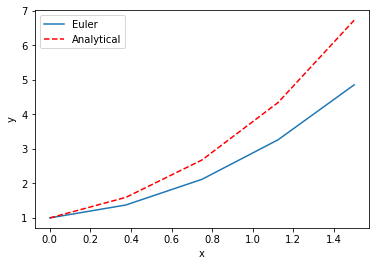
\includegraphics[width=.9\linewidth]{obipy-resources/744bcb3e58866fd0750c7a1efd9d42e8-68311E4V.png}
\end{center}

This solution does not look that good until you increase the number of points (i.e. decrease the value of \(h\), significantly). It is known the error decreases only linearly with \(h\).

\textbf{Exercise} Increase the number of points in the x array and see how it affects the solution.

This method is not used in practice; it is not very accurate, and you need quite small \(h\) to get a good solution. It is used here to illustrate the idea of how one integrates a differential equation. We will consider one more advanced method, the fourth-order Runge-Kutta method.

\subsubsection{Fourth-order Runge-Kutta method}
\label{sec:org2c40da2}

The general idea of the more advanced methods is to use a weighted average of slopes at various points around a point to best estimate the next function value. Here we consider the fourth-order Runge-Kutta algorithm. The terms are tedious to derive, and we will not do it here as they can be looked up in several places (e.g. \url{https://en.wikipedia.org/wiki/Runge\%E2\%80\%93Kutta\_methods\#The\_Runge\%E2\%80\%93Kutta\_method}).

\begin{minted}[frame=lines,fontsize=\scriptsize,linenos]{ipython}
x0 = 0
y0 = 1

x, h = np.linspace(x0, 1.5, 5, retstep=True)
print(f'h = {h}')
y = np.zeros(x.shape)
y[0] = y0

# Implementation of fourth order Runge Kutta method
for i in range(0, len(x) - 1):
    k1 = h * f(x[i], y[i]) # Note this is like Euler's method
    k2 = h * f(x[i] + h / 2, y[i] + k1 / 2)  # This is the increment at the midpoint using y, k1
    k3 = h * f(x[i] + h / 2, y[i] + k2 / 2)  # This is the increment at the midpoint using y, k2
    k4 = h * f(x[i + 1], y[i] + k3) # This is the increment at the end of the interval
    # This is a weighted average of the four increments computed above. There is a heavier weight on the midpoints
    y[i + 1] = y[i] + (k1 + (2 * k2) + (2 * k3) + k4) / 6
\end{minted}

\begin{verbatim}
h = 0.375

\end{verbatim}

\begin{minted}[frame=lines,fontsize=\scriptsize,linenos]{ipython}
plt.plot(x, y, label='RK-4')
plt.plot(x, x**2 + np.exp(x), 'r--', label='Analytical')
plt.xlabel('x')
plt.ylabel('y')
plt.legend()
\end{minted}

\begin{center}
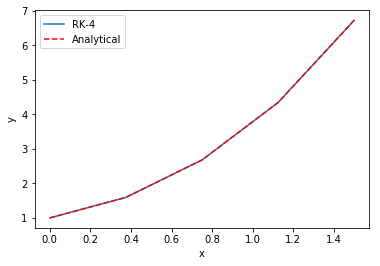
\includegraphics[width=.9\linewidth]{obipy-resources/744bcb3e58866fd0750c7a1efd9d42e8-68311RCc.png}
\end{center}


Note you can get a much more accurate solution with a larger \(h\) with this method.

\emph{If} our differential equation is just \(\frac{dy}{dt} = f(x)\), i.e. \(f\) is independent of \(y\), then this method is equivalent to Simpson't rule of integration.

Both of these methods leave some things to be desired:

\begin{enumerate}
\item We had to code them, and there are many places to make mistakes.
\item You have to choose \(h\), or equivalently the number of points to use, and then make sure the solution has converged (does not depend on your choice).
\item \(h\) is fixed in these examples, and you might prefer to use an adaptive value.
\item It is not easy to solve the inverse problem, e.g. for what value of \(x\) does \(y=4\)?
\end{enumerate}

In practice, there are well-written ODE integrators to solve this kind of problem that address all the short-comings listed above. To use them, we just need to learn the syntax. We do that next.

\subsection{scipy.integrate.solve\_ivp}
\label{sec:org5ae30b3}

The \texttt{scipy.integrate} library provides \texttt{solve\_ivp} to solve first order differential equations. It is not the only one available, but this function is recommended. You import the function like this:

\begin{minted}[frame=lines,fontsize=\scriptsize,linenos]{ipython}
from scipy.integrate import solve_ivp
\end{minted}

Here is a minimal use of the function, with keyword arguments.


\texttt{y0} is an array containing the initial values.  \texttt{fun} is a function with a signature of f(t, y). Here, \(t\) is considered the independent variable. You can call it whatever you want, so f(x, y) is also fine. Since \texttt{solve\_ivp} had \(t\) in mind, the second argument is the \texttt{t\_span}, which is a tuple of two numbers for where the integration starts (t0, or x0) and where it ends.  \texttt{solve\_ivp} returns an object.

\begin{minted}[frame=lines,fontsize=\scriptsize,linenos]{ipython}
y0 = np.array([y0]) # It is a good idea to make y0 an array. It will be important later.
sol = solve_ivp(fun=f, t_span=(x0, 1.5), y0=y0)
\end{minted}

The output of \texttt{solve\_ip} is an object containing results in attributes on the object.

\begin{minted}[frame=lines,fontsize=\scriptsize,linenos]{ipython}
sol
\end{minted}

\begin{verbatim}
 message: 'The solver successfully reached the interval end.'
    nfev: 20
    njev: 0
     nlu: 0
     sol: None
  status: 0
 success: True
       t: array([ 0.        ,  0.08034384,  0.86683456,  1.5       ])
t_events: None
       y: array([[ 1.        ,  1.09011474,  3.13086569,  6.73191444]])
\end{verbatim}

You should look for a few things here. One is that the message indicates success. Second, we access the solution using dot notation. Here are the independent variable values the solution was evaluated at.

\begin{minted}[frame=lines,fontsize=\scriptsize,linenos]{ipython}
sol.t
\end{minted}

\begin{verbatim}
array([ 0.        ,  0.08034384,  0.86683456,  1.5       ])
\end{verbatim}

Third, the solution is in a 2D array. We only have one equation here, so we use indexing to get the first row as an array.

\begin{minted}[frame=lines,fontsize=\scriptsize,linenos]{ipython}
sol.y[0]
\end{minted}

\begin{verbatim}
array([ 1.        ,  1.09011474,  3.13086569,  6.73191444])
\end{verbatim}

Now, we can plot the solution.

\begin{minted}[frame=lines,fontsize=\scriptsize,linenos]{ipython}
plt.plot(sol.t, sol.y[0], label='solve_ivp')
plt.plot(sol.t, sol.t**2 + np.exp(sol.t), 'r--', label='Analytical')
plt.xlabel('x')
plt.ylabel('y')
plt.legend()
\end{minted}

\begin{center}
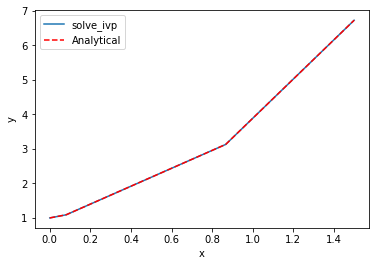
\includegraphics[width=.9\linewidth]{obipy-resources/744bcb3e58866fd0750c7a1efd9d42e8-68311eMi.png}
\end{center}

That doesn't looks so great since there are only four data points. By default, the algorithm only uses as many points as it needs to achieve a specified tolerance. We can specify that we want the solution evaluated at other points using the optional \texttt{t\_eval} keyword arg.

\begin{minted}[frame=lines,fontsize=\scriptsize,linenos]{ipython}
X = np.linspace(x0, 1.5)
sol = solve_ivp(fun=f, t_span=(x0, 1.5), y0=y0, t_eval=X)
sol
\end{minted}

\begin{verbatim}
 message: 'The solver successfully reached the interval end.'
    nfev: 20
    njev: 0
     nlu: 0
     sol: None
  status: 0
 success: True
       t: array([ 0.        ,  0.03061224,  0.06122449,  0.09183673,  0.12244898,
       0.15306122,  0.18367347,  0.21428571,  0.24489796,  0.2755102 ,
       0.30612245,  0.33673469,  0.36734694,  0.39795918,  0.42857143,
       0.45918367,  0.48979592,  0.52040816,  0.55102041,  0.58163265,
       0.6122449 ,  0.64285714,  0.67346939,  0.70408163,  0.73469388,
       0.76530612,  0.79591837,  0.82653061,  0.85714286,  0.8877551 ,
       0.91836735,  0.94897959,  0.97959184,  1.01020408,  1.04081633,
       1.07142857,  1.10204082,  1.13265306,  1.16326531,  1.19387755,
       1.2244898 ,  1.25510204,  1.28571429,  1.31632653,  1.34693878,
       1.37755102,  1.40816327,  1.43877551,  1.46938776,  1.5       ])
t_events: None
       y: array([[ 1.        ,  1.03202273,  1.06688599,  1.10462029,  1.14526069,
        1.18883821,  1.23538386,  1.28493005,  1.33751066,  1.39316097,
        1.45191772,  1.51381907,  1.57890465,  1.64721547,  1.71879402,
        1.79368421,  1.87193138,  1.95358232,  2.03868524,  2.12728979,
        2.21944707,  2.31520959,  2.41463131,  2.51776762,  2.62467537,
        2.7354128 ,  2.85003963,  2.96861698,  3.09120744,  3.21787836,
        3.34870553,  3.48375748,  3.6231049 ,  3.76682143,  3.91498364,
        4.06767101,  4.22496595,  4.38695382,  4.55372287,  4.7253643 ,
        4.90197223,  5.08364371,  5.2704787 ,  5.46258012,  5.66005377,
        5.86300842,  6.07155575,  6.28581035,  6.50588976,  6.73191444]])
\end{verbatim}

\begin{minted}[frame=lines,fontsize=\scriptsize,linenos]{ipython}
plt.plot(sol.t, sol.y[0], label='solve_ivp')
plt.plot(X, X**2 + np.exp(X), 'r--', label='Analytical')
plt.xlabel('x')
plt.ylabel('y')
plt.legend()
\end{minted}

\begin{center}
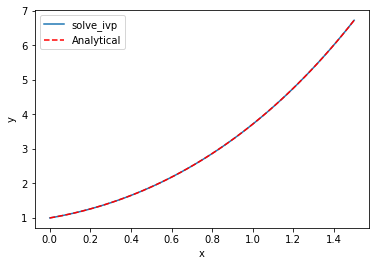
\includegraphics[width=.9\linewidth]{obipy-resources/744bcb3e58866fd0750c7a1efd9d42e8-181qOL.png}
\end{center}

So far, \texttt{solve\_ivp} solves the issues with item 1 (we did not have to code the algorithm), and items 2 and 3 (it uses an adaptive step and converges to a tolerance for us). It will also help us solve for the inverse problem, i.e. for what value of \(x\) is \(y=4\)?

To do this, we need a new concept of an "event function". During each step of the integration, you can run a function that can detect an "event". When an event is detected, the location of the event is stored, and if desired integration can be terminated. \texttt{solve\_ivp} can take a list of event functions. We consider only one for now.

An event occurs when an event function is equal to zero. During integration, if the event function changes sign, then it is clear an event has occurred, and the algorithm determines where it occurred. Since we want to know when \(y=4\), we will define a function that returns \(y - 4\), because that will equal zero at that condition. We want the integration to terminate when that happens, so we set the "terminal" attribute on our function to True.

An event function has a signature of f(x, y). Remember that \(y\) is going to be an array,

\begin{minted}[frame=lines,fontsize=\scriptsize,linenos]{ipython}
def event1(x, y):
    return y[0] - 4

event1.terminal = True

sol = solve_ivp(fun=f, t_span=(x0, 1.5), y0=y0, events=event1)
sol
\end{minted}

\begin{verbatim}
 message: 'A termination event occurred.'
    nfev: 20
    njev: 0
     nlu: 0
     sol: None
  status: 1
 success: True
       t: array([ 0.        ,  0.08034384,  0.86683456,  1.05797402])
t_events: [array([ 1.05797402])]
       y: array([[ 1.        ,  1.09011474,  3.13086569,  4.        ]])
\end{verbatim}

Now, there are a couple of new things to note. First, we got a message that a termination event occurred. Second, the sol.y array ends at 4.0, because we made the event function \emph{terminal}. Next, sol.t\_events is not empty, because an event occurred. It now contains the value where the event occurred, which is where \(y=4\)!

\begin{minted}[frame=lines,fontsize=\scriptsize,linenos]{ipython}
sol.t_events[0]
\end{minted}

\begin{verbatim}
array([ 1.05797402])
\end{verbatim}

\begin{minted}[frame=lines,fontsize=\scriptsize,linenos]{ipython}
sol.t
\end{minted}

\begin{verbatim}
array([ 0.        ,  0.08034384,  0.86683456,  1.05797402])
\end{verbatim}

\begin{minted}[frame=lines,fontsize=\scriptsize,linenos]{ipython}
print(f'y=4 at x={sol.t[-1]}. Confirming: y = {sol.t[-1]**2 + np.exp(sol.t[-1])}')
\end{minted}

\begin{verbatim}
y=4 at x=1.0579740235381914. Confirming: y = 3.9998382237380805

\end{verbatim}


That is pretty close. You have to decide if it is close enough for the purpose you want. You can control the tolerance with optional \texttt{atol} and \texttt{rtol} keywords. You should read the documentation before changing this.

\begin{minted}[frame=lines,fontsize=\scriptsize,linenos]{ipython}
def event1(x, y):
    return y[0] - 4

event1.terminal = True

sol = solve_ivp(fun=f, t_span=(x0, 1.5), y0=y0, events=event1, rtol=1e-9)
sol
sol.t[-1]**2 + np.exp(sol.t[-1])
\end{minted}

\begin{verbatim}
3.9999993427868006
\end{verbatim}

\subsection{Summary}
\label{sec:org960b50a}

We learned how to solve different types of first-order differential equations. Linear equations can be solved by integration, which has the benefit of providing an estimate of error if the \texttt{scipy.integrate.quad} function is used.

Most first-order differential equations can be solved numerically with \texttt{scipy.integrate.solve\_ivp}. This solver allows you to specify the points the solution is evaluated on, and to define event functions that can terminate the integration, or record where events occur.

\section{04 First-order differential equations - part 2}
\label{sec:org1940843}

\subsection{Families of solutions to FODEs}
\label{sec:orgdaaeb9a}

Consider \(y' = x - y\).

We can interpret this equation as one that defines a direction field. That is, at any given point (x, y) we can compute the derivative of a solution at that point. We will consider how to make a plot that shows this field, and that will help us estimate what solutions to the ODE might look like for different initial values.

To do this, we should compute the derivative on an array of regularly spaced points in both \(x\) and \(y\), and then making a plot of that data.

We need to see a couple of new ideas to make this plot efficiently. What we want is a 2-d plot of a regular grid of (x, y) points, and at each of those points the derivative (dx/dx, dy/dx).

First, we will need to create four arrays:
\begin{enumerate}
\item a 2d array of all the x-positions
\item a 2d array of all the y-positions
\item a 2d array of the dx/dx = 1 values
\item a 2d array of the dy/dx values.
\end{enumerate}

We want to generate the x, y arrays. We use \texttt{np.meshgrid} for this. The simplest way to do it is to use \texttt{np.linspace} to create 1-D arrays with the spacing we want, and then use \texttt{np.meshgrid} to generate the 2D arrays. Let's say we want a uniform grid over the range of x from 0 to 1, and over the range of y from 0 to 3, with 5 points in each direction.

\begin{minted}[frame=lines,fontsize=\scriptsize,linenos]{ipython}
import numpy as np

x = np.linspace(0, 1, 5)
y = np.linspace(0, 3, 5)

X, Y = np.meshgrid(x, y)
X, Y
\end{minted}

\begin{verbatim}
(array([[ 0.  ,  0.25,  0.5 ,  0.75,  1.  ],
        [ 0.  ,  0.25,  0.5 ,  0.75,  1.  ],
        [ 0.  ,  0.25,  0.5 ,  0.75,  1.  ],
        [ 0.  ,  0.25,  0.5 ,  0.75,  1.  ],
        [ 0.  ,  0.25,  0.5 ,  0.75,  1.  ]]),
 array([[ 0.  ,  0.  ,  0.  ,  0.  ,  0.  ],
        [ 0.75,  0.75,  0.75,  0.75,  0.75],
        [ 1.5 ,  1.5 ,  1.5 ,  1.5 ,  1.5 ],
        [ 2.25,  2.25,  2.25,  2.25,  2.25],
        [ 3.  ,  3.  ,  3.  ,  3.  ,  3.  ]]))
\end{verbatim}

Now, we have X, Y arrays that map out all the (x, y) pairs we want to consider. So, the (x, y) pair in the second row and third column of the array is:

\begin{minted}[frame=lines,fontsize=\scriptsize,linenos]{ipython}
(X[1, 2], Y[1, 2])
\end{minted}

\begin{verbatim}
(0.5, 0.75)
\end{verbatim}

These are arrays, so we can do math with them.

\begin{minted}[frame=lines,fontsize=\scriptsize,linenos]{ipython}
X - Y
\end{minted}

\begin{verbatim}
array([[ 0.  ,  0.25,  0.5 ,  0.75,  1.  ],
       [-0.75, -0.5 , -0.25,  0.  ,  0.25],
       [-1.5 , -1.25, -1.  , -0.75, -0.5 ],
       [-2.25, -2.  , -1.75, -1.5 , -1.25],
       [-3.  , -2.75, -2.5 , -2.25, -2.  ]])
\end{verbatim}

\begin{minted}[frame=lines,fontsize=\scriptsize,linenos]{ipython}
np.sqrt(X**2 + Y**2)
\end{minted}

\begin{verbatim}
array([[ 0.        ,  0.25      ,  0.5       ,  0.75      ,  1.        ],
       [ 0.75      ,  0.79056942,  0.90138782,  1.06066017,  1.25      ],
       [ 1.5       ,  1.52069063,  1.58113883,  1.67705098,  1.80277564],
       [ 2.25      ,  2.26384628,  2.30488611,  2.37170825,  2.46221445],
       [ 3.        ,  3.01039864,  3.04138127,  3.09232922,  3.16227766]])
\end{verbatim}


Now we are ready to compute a distance field for the FODE. We will consider the range from -1 to 1 in both x and y, and then plot the results with \texttt{matplotlib.pyplot.quiver}.

\begin{minted}[frame=lines,fontsize=\scriptsize,linenos]{ipython}
%matplotlib inline
import matplotlib.pyplot as plt
\end{minted}

Review the documentation for this function:

\begin{minted}[frame=lines,fontsize=\scriptsize,linenos]{ipython}
?plt.quiver
\end{minted}

We define the ode function, create the grids, and then make the plot.

\begin{minted}[frame=lines,fontsize=\scriptsize,linenos]{ipython}
def yprime(x, y):
    return x - y

x = np.linspace(-1, 1, 20)
y = np.linspace(-1, 1, 20)

X, Y = np.meshgrid(x, y)
U = np.ones(X.shape)  # dx/dx
V = yprime(X, Y)  # dy/dx

# This normalizes the arrows so they are all the same length
N = np.sqrt(U**2 + V**2)
U /= N
V /= N

plt.quiver(X, Y, U, V)
plt.xlabel('x')
plt.ylabel('y')
\end{minted}

\begin{center}
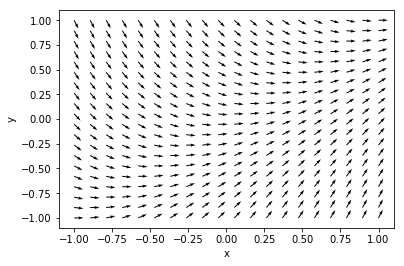
\includegraphics[width=.9\linewidth]{obipy-resources/05b8b46ebbc2df3b9d545d77190f5234-683117xr.png}
\end{center}

If you pick a point, the arrows show you which way the solution goes from there. You just follow the arrows to get an approximate solution to this equation. Let's consider some specific solutions. Suppose we start with the initial condition that \(y(-1) = 0\). You can trace the arrows to estimate where the solution goes.

Let us use a numerical solver to see how it works.

\begin{minted}[frame=lines,fontsize=\scriptsize,linenos]{ipython}
from scipy.integrate import solve_ivp

sol = solve_ivp(yprime, (-1, 1), (0,), t_eval=np.linspace(-1, 1))
sol.message  # you should at least check this message to see if it worked.
\end{minted}

\begin{verbatim}
'The solver successfully reached the interval end.'
\end{verbatim}

Now, we plot the solution

\begin{minted}[frame=lines,fontsize=\scriptsize,linenos]{ipython}
plt.plot(sol.t, sol.y[0], 'r', lw=2)
plt.quiver(X, Y, U, V)
plt.xlabel('x')
plt.ylabel('y')
\end{minted}

\begin{center}
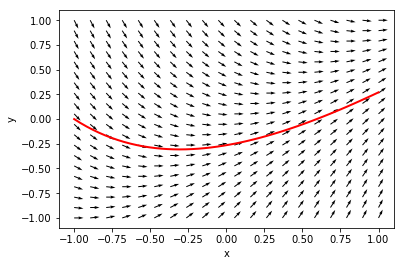
\includegraphics[width=.9\linewidth]{obipy-resources/05b8b46ebbc2df3b9d545d77190f5234-68311I8x.png}
\end{center}

Here are some more examples.

\begin{minted}[frame=lines,fontsize=\scriptsize,linenos]{ipython}
sol2 = solve_ivp(yprime, (-0.5, 1), (0.5,), t_eval=np.linspace(-0.5, 1))
sol3 = solve_ivp(yprime, (0.0, 1), (-1,), t_eval=np.linspace(0.0, 1))
sol4 = solve_ivp(yprime, (0.0, 1), (1,), t_eval=np.linspace(0.0, 1))

plt.plot(sol2.t, sol2.y[0], 'r', lw=2)
plt.plot(sol3.t, sol3.y[0], 'g', lw=2)
plt.plot(sol4.t, sol4.y[0], 'b', lw=2)

# overlay the direction field
plt.quiver(X, Y, U, V)
plt.xlabel('x')
plt.ylabel('y')
\end{minted}

\begin{center}
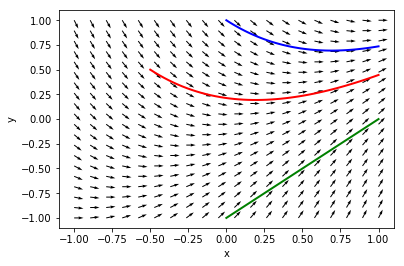
\includegraphics[width=.9\linewidth]{obipy-resources/05b8b46ebbc2df3b9d545d77190f5234-683116FB.png}
\end{center}

You can see the solution looks different depending on the initial condition, but in each case the solution follows the direction field.

Direction field plots can be very helpful to visualize what nearby solutions might look like, or to get a qualitative idea of what a solution might look like, or to see if anything unusual happens in the solution space. We will see them again when we consider systems of differential equations.

\textbf{Exercise:} Make a direction field plot for \(y'=-y\) for the range of x from 0 to 4. What does the direction field tell you? How does this compare to what you know from the solution?

\subsection{Systems of first-order differential equations}
\label{sec:org969f4e7}

Many engineering systems are governed by \emph{systems of coupled} differential equations. This usually means there are two or more independent variables and outputs, and the rate of change of the outputs depends on two or more of the independent variables.

Let's consider the following tank mixing problem. You have two tanks: Tank A has 30 gallons containing 55 ounces of dissolved salt, and Tank B has 20 gallons containing 26 ounces of salt. Additionally,

\begin{itemize}
\item Water with a salt concentration of 1 oz/gal flows into Tank A at a rate of 1.5 gal/min.
\item Water with a salt concentration of 3 oz/gal flows into Tank B at a rate of 1 gal/min
\item Water flows from Tank A to Tank B at a rate of 3 gal/min.
\item Water flows from Tank B to Tank A at a rate of 1.5 gal/min
\item Water drains from Tank B at a rate of 2.5 gal/min.
\end{itemize}

\url{two-tank-mixing.png}

Plot the concentration of salt in Tank A and B as a function of time.

First, we can define initial conditions.

\begin{minted}[frame=lines,fontsize=\scriptsize,linenos]{ipython}
V_A = 30 # gal
V_B = 20 # gal

S_A0 = 55 / V_A # oz/gallon in Tank A at T=0
S_B0 = 26 / V_B # oz/gallon in Tank B at T=0

S_A0, S_B0
\end{minted}

\begin{verbatim}
(1.8333333333333333, 1.3)
\end{verbatim}

Now, let's define the flow rates and check the net volumetric flow into each tank.

\begin{minted}[frame=lines,fontsize=\scriptsize,linenos]{ipython}
f_A = 1.5 # volumetric flow into A gal/min
C_A = 1   # salt concentration in flow oz/gal

f_B = 1.0 # volumetric flow into B, gal/min
C_B = 3   # salt concentration into B, oz/gal

f_AB = 3 # flow from A to B, gal/min
f_BA = 1.5 # flow from B to A, gal/min

f_Bexit = 2.5  # flow out of B

print(f'Net flow into A = {f_A - f_AB + f_BA} gal/min')
print(f'Net flow into B = {f_B + f_AB - f_BA - f_Bexit} gal/min')
\end{minted}

\begin{verbatim}
Net flow into A = 0.0 gal/min
Net flow into B = 0.0 gal/min

\end{verbatim}

You can see the net volumetric flow in each tank is 0, so we do not have to worry about the volumes changing.

We seek solutions for \(S_A(t)\) and \(S_B(t)\) where \(S_x(t)\) represents the concentration (in oz/gal). Since these change with time, we need to solve the mass balances:

\(\frac{dS_A}{dt} = \frac{1}{V_A}(f_A C_A - f_{AB} S_A(t) + f_{BA} S_B(t))\)

and

\(\frac{dS_B}{dt} = \frac{1}{V_B}(f_B C_B + f_{AB} S_A(t) - F_{BA} S_B(t) - F_{Bexit} S_B(t))\)

Before we get into the solution, what should we expect to happen here? The concentration of salt into tank A is less than the initial concentration, and the initial concentration in Tank B is also lower than in Tank A, so we expect the concentration in Tank A to start decreasing. Similarly, we expect the concentration in Tank B to start rising since the concentration in each incoming stream is higher than the initial concentration.

At some point, the two tanks will reach a steady state, but it is not evident how we will approach that steady state. Since the concentration of one stream is higher than all the other concentrations, it is possible for the concentration to go up and then down.

\begin{minted}[frame=lines,fontsize=\scriptsize,linenos]{ipython}
def dSdt(t, S):
    S_A = S[0]
    S_B = S[1]
    dSadt = (f_A * C_A - f_AB * S_A + f_BA * S_B) / V_A
    dSbdt = (f_B * C_B + f_AB * S_A - f_BA * S_B - f_Bexit * S_B) / V_B
    return np.array([dSadt, dSbdt])

from scipy.integrate import solve_ivp

S0 = np.array([S_A0, S_B0])
tspan = np.array([0, 200])

# there is a new syntax here. *tspan means to "unpack" tspan into this position
# it is equivalent to:
# teval = np.linspace(tspan[0], tspan[1], 100)
teval = np.linspace(*tspan, 100)

sol = solve_ivp(dSdt, tspan, S0, t_eval=teval)
\end{minted}

The shape of our solution is two rows by 50 columns.

\begin{minted}[frame=lines,fontsize=\scriptsize,linenos]{ipython}
sol.y.shape
\end{minted}

\begin{verbatim}
(2, 100)
\end{verbatim}


One way to plot these solutions is this, where we extract out each row of the solution:

\begin{minted}[frame=lines,fontsize=\scriptsize,linenos]{ipython}
%matplotlib inline
import matplotlib.pyplot as plt
plt.plot(sol.t, sol.y[0] * V_A, label='Tank A')
plt.plot(sol.t, sol.y[1] * V_B, label='Tank B')
plt.xlabel('t (min)')
plt.ylabel('Mass of salt (oz)')
plt.legend()
\end{minted}

\begin{center}
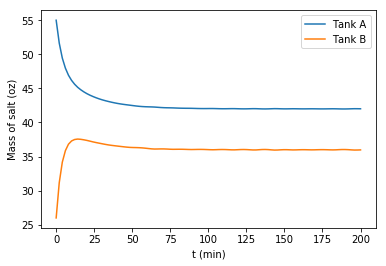
\includegraphics[width=.9\linewidth]{obipy-resources/05b8b46ebbc2df3b9d545d77190f5234-68311G6j.png}
\end{center}

Another way is to convert the solution to an array where the data we want to plot is in columns. We can achieve this by \emph{transposing} the array to convert it from 2 rows with 50 columns to 50 rows with 2 columns.

\begin{minted}[frame=lines,fontsize=\scriptsize,linenos]{ipython}
sol.y.T.shape
\end{minted}

\begin{verbatim}
(100, 2)
\end{verbatim}


Now, we can also multiply each row by the volumes to get the mass of salt in each tank.

\begin{minted}[frame=lines,fontsize=\scriptsize,linenos]{ipython}
plt.plot(sol.t, sol.y.T * [V_A, V_B])
plt.xlabel('t (min)')
plt.ylabel('Mass of salt (oz)')
plt.legend(['Tank A', 'Tank B'])
\end{minted}

\begin{center}
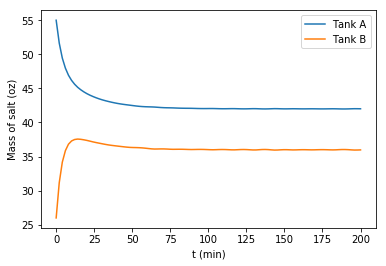
\includegraphics[width=.9\linewidth]{obipy-resources/05b8b46ebbc2df3b9d545d77190f5234-68311TEq.png}
\end{center}


This works because you can plot an array where the values to be plotted are all in columns.

\subsubsection{Brief review}
\label{sec:org9e3a7d2}

For systems of first order differential equations, you need to:

\begin{enumerate}
\item Define a function \(y'(t, y)\) where \(y\) will be an array of values. The function must return an array that is the same shape as \(y\). For example, if you have two equations, \(y\) will contain the two function values, and \(y'\) must return two derivative values.
\item You also need two initial conditions, one for each function, at the same value of \(t\).
\item The solution from solve\_ivp will return an array for the y-values, with each function in \emph{a row} of that array. You can either extract the rows to plot them, or transpose the array and plot them all.
\end{enumerate}

\subsubsection{Predator-prey model example}
\label{sec:org741913d}

The Lotka-Volterra model can be used to simulate predator-prey populations. Suppose we have \(u\) preys (e.g. rabbits) and \(v\) predators (e.g. foxes). Then, we can do a "mass balance" on each species as

\(\frac{du}{dt} = a u - b u v\)

\(\frac{dv}{dt} = -c v + d b u v\)

Here \(a\) is the natural growth rate of rabbits with no foxes. \(b\) is the rate that foxes eat rabbits. \(c\) is the rate that foxes die, and \(d\) describes how many new foxes result from the rabbits that are eaten. Suppose we start with 10 rabbits and 5 foxes. Plot the number of each species from t=0 to t=15.

\begin{minted}[frame=lines,fontsize=\scriptsize,linenos]{ipython}
a = 1.
b = 0.1
c = 1.5
d = 0.75

Y0 = np.array([10, 5])
tspan = (0, 15)
teval = np.linspace(*tspan, 1500)

def dXdt(t, X):
    rabbits, foxes = X
    drabbitdt = a * rabbits - b * rabbits * foxes
    dfoxesdt = -c * foxes + d * b * rabbits * foxes
    return np.array([drabbitdt, dfoxesdt])

from scipy.integrate import solve_ivp
sol = solve_ivp(dXdt, tspan, Y0, t_eval=teval)
sol.message
\end{minted}

\begin{verbatim}
'The solver successfully reached the interval end.'
\end{verbatim}

\begin{minted}[frame=lines,fontsize=\scriptsize,linenos]{ipython}
plt.plot(sol.t, sol.y.T)
plt.ylim([0, 50])
plt.legend(['rabbits', 'foxes'], loc='upper right')
plt.xlabel('t')
plt.ylabel('count')
plt.xlim(tspan)
\end{minted}

\begin{verbatim}
(0, 15)
\end{verbatim}



\begin{center}
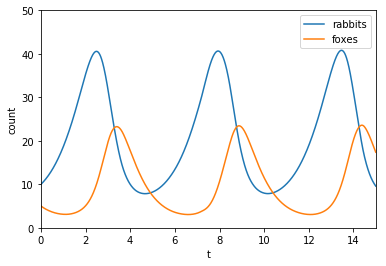
\includegraphics[width=.9\linewidth]{obipy-resources/05b8b46ebbc2df3b9d545d77190f5234-68311UaN.png}
\end{center}

This is a classic boom/bust cycle of predator/prey.

\subsubsection{Qualitative method for systems of ODEs}
\label{sec:org10c0153}

We can consider direction fields for systems of ODEs to examine the qualitative behavior of solutions when there are two equations. The key here is to compute for each point (rabbit, fox) we compute (drabbit/dt, dfox/dt), and then plot these.

\begin{minted}[frame=lines,fontsize=\scriptsize,linenos]{ipython}
r = np.linspace(0, 40, 20) # rabbit grid
f = np.linspace(0, 40, 20) # fox grid

R, F = np.meshgrid(r, f) # 2D arrays of (rabbit, fox) points

DR, DF = dXdt(0, [R, F])

# This normalizes the arrows so they are all the same length and just show the direction
N = np.sqrt(DR**2 + DF**2)
N[N==0] = 1 # eliminate / 0 errors, it is sort of optional.
DR /= N
DF /= N

plt.quiver(R, F, DR, DF)
plt.xlabel('Number of rabbits')
plt.ylabel('Number of foxes')
plt.plot(sol.y[0], sol.y[1]);
\end{minted}

\begin{center}
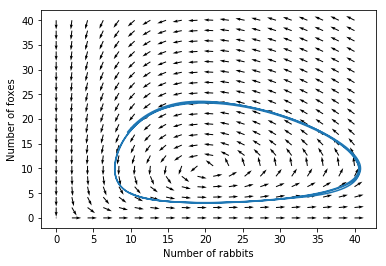
\includegraphics[width=.9\linewidth]{obipy-resources/05b8b46ebbc2df3b9d545d77190f5234-68311ugx.png}
\end{center}

In this view, we have a \emph{limit cycle} which just shows the number of rabbits and foxes goes up and down periodically as you travel around the solution curve. Time is parametric in this plot. It starts at t=0 at the initial state, and increases as you go around the cycle.

\subsection{Summary}
\label{sec:org0bd9b3f}

Systems of first order differential equations are solved the same way as single first order differential equations. The main difference is the system must be defined as:

\(Y'(t) = f(x, Y)\)

where \(Y'\) is a vector/array of first derivatives, and \(Y\) is a vector/array of function values.

You still use \texttt{scipy.integrate.solve\_ivp} to solve the equations, but you need an initial condition for each equation.

<div class="alert alert-warning">
There are other ode integrators in scipy that have different function signatures than \texttt{scipy.integrate.solve\_ivp}.

For example, \texttt{scipy.integrate.odeint} requires functions like \(y' = f(y, t)\) which is the opposite of \texttt{scipy.integrate.solve\_ivp}. You \textbf{have} to keep track of which one you are using.

\texttt{scipy.integrate.odeint} is older than \texttt{scipy.integrate.solve\_ivp}, but it has fewer features (e.g. no events, fewer solver options).
</div>

\section{05 N\(^{\text{th}}\) order differential equations}
\label{sec:orgb75f823}
So far we have focused on computational solutions to first order differential equations, including systems of first order differential equations. The reason for that is simply that all numerical integration strategies only work with the first derivative.

Many differential equations involve higher order derivatives though. We can solve these by converting them to systems of first-order differential equations through a series of variable changes.

Let's consider the \href{https://en.wikipedia.org/wiki/Van\_der\_Pol\_oscillator}{Van der Pol oscillator}.

\(\frac{d^2x}{dt^2} - \mu(1-x^2)\frac{dx}{dt} + x = 0\)

We define a new variable: \(v = x'\), and then have \(v' = x''\).

That leads to a set of equivalent first-order differential equations:

\(x' = v\)

\(v' - \mu (1-x^2)v + x = 0\)

You can still think of \(x\) as the position of the oscillator, and \(y\) as the velocity of the oscillator. Now, we can integrate these equations from some initial condition.

Let's do this and plot the position and velocity of the oscillator. Rather than use \texttt{t\_eval}, we will instead set the optional argument \texttt{max\_step} to tell the solver how often it should make a step.

This is different than using \texttt{t\_eval}, which uses interpolation \emph{after} the solution has been found to evaluate the solution. This will become important later when we use events, which are only evaluated at the \emph{solver} points.

\begin{minted}[frame=lines,fontsize=\scriptsize,linenos]{ipython}
import numpy as np
from scipy.integrate import solve_ivp

mu = 0.2

def dXdt(t, X):
    x, v = X
    dxdt = v
    dvdt = mu * (1 - x**2) * v - x
    return np.array([dxdt, dvdt])

X0 = np.array((1, 2)) # you can pick any x0, and v0 you want.
tspan = np.array((0, 40))
teval, h = np.linspace(*tspan, 500, retstep=True)

sol = solve_ivp(dXdt, tspan, X0, max_step=h)
sol.message, sol.success
\end{minted}

\begin{verbatim}
('The solver successfully reached the end of the integration interval.', True)
\end{verbatim}

Now, we can plot the solutions.

\begin{minted}[frame=lines,fontsize=\scriptsize,linenos]{ipython}
%matplotlib inline
import matplotlib.pyplot as plt

plt.plot(sol.t, sol.y.T);
plt.xlabel('t')
plt.ylabel('x,v')
plt.legend(['x', 'v'])
\end{minted}

\begin{center}
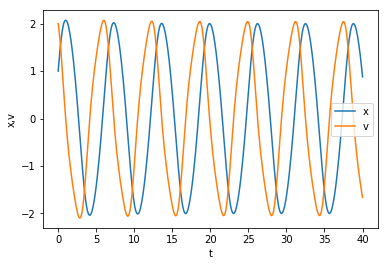
\includegraphics[width=.9\linewidth]{obipy-resources/c515c00ecd6370edf5b32608ff70731e-388473FS.png}
\end{center}

You can see that the solution appears oscillatory. Let's be more quantitative than what it \emph{looks} like. An alternative way to visualize this solution is called the phase portrait where we plot the two state variables (x, v) against each other. We include the starting point for visualization.

\begin{minted}[frame=lines,fontsize=\scriptsize,linenos]{ipython}
plt.plot(*sol.y)
plt.plot(*sol.y[:, 0], 'go') # starting point
plt.xlabel('x')
plt.ylabel('v')
plt.axis('equal');
\end{minted}

\begin{center}
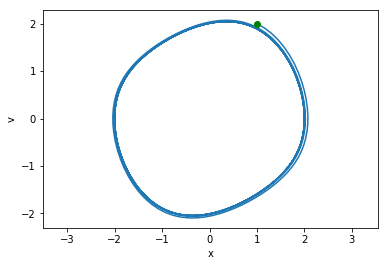
\includegraphics[width=.9\linewidth]{obipy-resources/c515c00ecd6370edf5b32608ff70731e-38847p6E.png}
\end{center}

So, evidently it is not exactly periodic in the beginning, but seems to take some time to settle down into a periodic rhythm. That seems to be the case, because if it didn't we would expect to see a continued spiral in or out of this limit cycle. Another way we can assess this quantitatively is to look at the peak positions in our solution. We return to an event type of solution. We seek an event where the derivative \(dx/dt=0\), and it is a maximum, which means \(x'\) starts positive, becomes zero, and then is negative. Note this is appropriate for this problem, where there is only one, periodic maximum. For other problems, you might need a different approach.

Now, it is important to remember that the event function is only evaluated after a solver point, so we need to make sure the solver points bracket where events occur. This is accomplished by making sure that when we graph the solution from the solver (not from t\_eval), that we can visually see where the events will occur.

We use a new optional argument, \texttt{dense\_output=True} in \texttt{solve\_ivp} which will let us evaluate the solution at the event times.

\begin{minted}[frame=lines,fontsize=\scriptsize,linenos]{ipython}
def max_x_event(t, X):
    x, v = X
    Xprime = dXdt(t, X)
    return Xprime[0]  # first derivative = 0

max_x_event.direction = -1 # event must go from positive to negative, i.e. a max

sol = solve_ivp(dXdt, tspan, X0, max_step=h, events=max_x_event, dense_output=True)
sol.t_events
\end{minted}

\begin{verbatim}
[array([  0.98712369,   7.29961546,  13.60207133,  19.90194032,
         26.2010961 ,  32.50005162,  38.79895061])]
\end{verbatim}

You can see we found seven events. We need to evaluate the solution at these points, and we should plot them on the solution to see that they are in fact maxima. (what could possibly go wrong? if you get the wrong direction, then you will either see minima, or minima and maxima! If your event function is wrong, then it will just be wrong.) When you use \texttt{dense\_output=True}, you get a new attribute on the solution which can be used to estimate the solution at some t values. Note we get two rows in our solution, one for x and one for v. From the numbers here, you can see that the x\_max values seem to be settling down to about 2.0.

\begin{minted}[frame=lines,fontsize=\scriptsize,linenos]{ipython}
sol.sol(sol.t_events[0])
\end{minted}

\begin{verbatim}
array([[  2.07283325e+00,   2.02004874e+00,   2.00590349e+00,
          2.00196134e+00,   2.00085100e+00,   2.00053732e+00,
          2.00044864e+00],
       [  0.00000000e+00,   5.84601811e-16,   5.82867088e-16,
         -3.21270788e-15,   2.44249065e-15,  -4.48252546e-15,
          6.62664368e-15]])
\end{verbatim}


\begin{minted}[frame=lines,fontsize=\scriptsize,linenos]{ipython}
plt.plot(sol.t, sol.y.T)

# break up this calculation for ease of reading
te = sol.t_events[0]
xmax, v_at_xmax = sol.sol(te)
plt.plot(te, xmax, 'ro')
plt.plot(te, v_at_xmax, 'bo')

# compare to. Don't do this, it is confusing and hard to figure out.
plt.plot(sol.t_events[0], sol.sol(sol.t_events[0])[0], 'ro')

plt.xlabel('t')
plt.ylabel('x,v')
plt.legend(['x', 'v'])

\end{minted}

\begin{center}
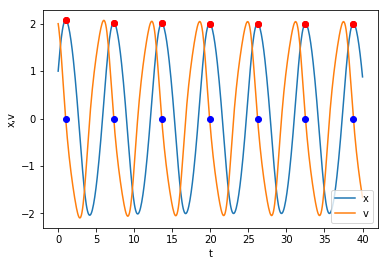
\includegraphics[width=.9\linewidth]{obipy-resources/c515c00ecd6370edf5b32608ff70731e-388472EL.png}
\end{center}

That looks good, the red dots appear at the maxima, and they are periodic, so now we can see how x\(_{\text{max}}\) varies with time.

\begin{minted}[frame=lines,fontsize=\scriptsize,linenos]{ipython}
plt.plot(te, xmax, 'ro')
plt.xlabel('t')
plt.ylabel('$x_{max}$')
\end{minted}

\begin{center}
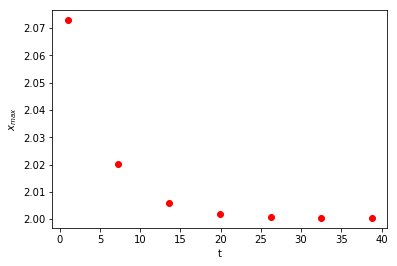
\includegraphics[width=.9\linewidth]{obipy-resources/c515c00ecd6370edf5b32608ff70731e-38847DPR.png}
\end{center}

You can see that after about 5 cycles, xmax is practically constant. We can also see that the period (the time between maxima) is converging to a constant. We cannot say much about what happens at longer times. You could integrate longer if it is important to know that. This is a limitation of numerical methods though. To \emph{prove} that it will be constant, you need to do some analytical math that would show the period and x\(_{\text{max}}\) go to a constant.

\begin{minted}[frame=lines,fontsize=\scriptsize,linenos]{ipython}
plt.plot(np.diff(te), 'bo')
plt.xlabel('cycle')
plt.ylabel('period')
\end{minted}

\begin{center}
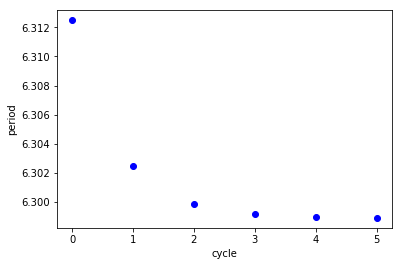
\includegraphics[width=.9\linewidth]{obipy-resources/c515c00ecd6370edf5b32608ff70731e-38847QZX.png}
\end{center}

If we seek the steady state, oscillatory behavior of this system, we should discard the solutions in at least the first 4 cycles, since the maxima and periods are still changing.

\begin{minted}[frame=lines,fontsize=\scriptsize,linenos]{ipython}
te[-1]
sol.sol(te[-1])
\end{minted}

\begin{verbatim}
array([  2.00044864e+00,   6.62664368e-15])
\end{verbatim}

Alternatively, we can use the last point as an initial value for a new integration that should be close to steady state oscillations.

\begin{minted}[frame=lines,fontsize=\scriptsize,linenos]{ipython}
tspan = (0, 40)
X0 = sol.sol(te[-1])

sol2 = solve_ivp(dXdt, tspan, X0, max_step=h, events=max_x_event)
plt.plot(sol2.t, sol2.y.T)
plt.xlabel('t')
plt.ylabel('x,v')
\end{minted}

\begin{center}
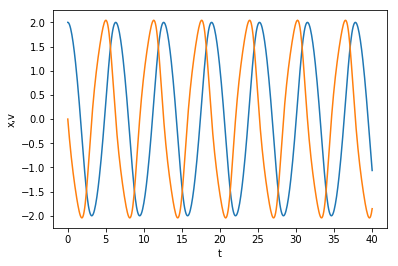
\includegraphics[width=.9\linewidth]{obipy-resources/c515c00ecd6370edf5b32608ff70731e-38847djd.png}
\end{center}

Here you see about 6 more cycles. The period of these events is practically constant.

\begin{minted}[frame=lines,fontsize=\scriptsize,linenos]{ipython}
sol2.t_events, np.diff(sol2.t_events[0])
\end{minted}

\begin{verbatim}
([array([  3.31307575e-15,   6.29888301e+00,   1.25977615e+01,
           1.88966387e+01,   2.51955156e+01,   3.14943923e+01,
           3.77932690e+01])],
 array([ 6.29888301,  6.2988785 ,  6.29887721,  6.29887685,  6.29887676,
         6.29887672]))
\end{verbatim}

And the limit cycle shows practically a single curve.

\begin{minted}[frame=lines,fontsize=\scriptsize,linenos]{ipython}
plt.plot(*sol2.y)
plt.xlabel('x')
plt.ylabel('y')
plt.axis('equal'); # makes x-ticks have the same dimension as y-ticks
\end{minted}

\begin{center}
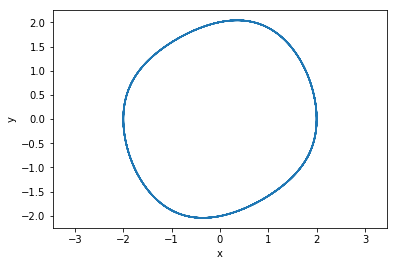
\includegraphics[width=.9\linewidth]{obipy-resources/c515c00ecd6370edf5b32608ff70731e-38847qtj.png}
\end{center}

This limit cycle shows the oscillatory behavior. You can see here that each cycle repeats on top of itself.

\textbf{Review} We have been working on finding a steady state oscillatory solution to \(\frac{d^2x}{dt^2} - \mu(1-x^2)\frac{dx}{dt} + x = 0\), which describes an oscillating system. We examined some ways to tell if a system is oscillating, and to estimate the period of the oscillation.

\subsection{Solving a parameterized ODE many times}
\label{sec:orgc665bf6}

\(\mu\) in the Van der Pol system is called a parameter. It is common to study the solution of this system as a function of \(\mu\). For \href{https://en.wikipedia.org/wiki/Van\_der\_Pol\_oscillator\#/media/File:VanderPol-lc.svg}{example}, the oscillatory behavior changes a lot as \(\mu\) changes. Our aim here is to recreate the figure in that example, showing the steady state limit cycles as a function of \(\mu\).

The example we want to create has limit cycles for 10 different values of \(\mu\). \emph{We do not want to copy and paste code 10 times}. Instead, we should have some code we can \emph{reuse 10 times}.

Let's break this task down. For a given \(\mu\), we should find a solution to the ODEs that shows constant periods. That means we should integrate over a time span, check the periods, and if they are not constant, integrate from the last point over the time span again. If they are consistent, then we can just plot the solution.

How can we check the periods are constant? One way is to see if the first and last are the same within some tolerance, say 1e-3.

Ideally, we would have a function that takes one argument, \(\mu\), and returns the steady state oscillatory solution.

\begin{minted}[frame=lines,fontsize=\scriptsize,linenos]{ipython}
# We do not have to define this here, I just repeat it so you can see it again.
def max_x_event(t, X):
    x, v = X
    Xprime = dXdt(t, X)
    return Xprime[0]  # first derivative = 0

max_x_event.direction = -1 # event must go from positive to negative, i.e. a max


def get_steady_state(mu):

    # define the sys odes for this mu. We define it inside the function so it
    # uses the mu passed in to get_steady_state.
    def dXdt(t, X):
        x, v = X
        dxdt = v
        dvdt = mu * (1 - x**2) * v - x
        return np.array([dxdt, dvdt])


    X0 = np.array([2, 0])  # start at x_max, velocity=0
    tspan = np.array([0, 40]) # we assume we will get 4-6 periods this way
    teval, h = np.linspace(*tspan, 1500, retstep=True)

    # initial solution
    sol = solve_ivp(dXdt, tspan, X0, max_step=h, events=max_x_event, dense_output=True)
    periods = np.diff(sol.t_events[0])

    # Now iterate as long as the first and last periods differ by more than the
    # tolerance. It is usually a good idea to provide a way to break out in case
    # it never ends. Here we use a max iteration count.
    i = 0

    # This assumes there are at least 2 periods in the tspan.
    while np.abs(periods[0] - periods[-1]) > 1e-3:
        last_step = sol.y[:, -1] # this is the new initial condition to continue from.
        sol = solve_ivp(dXdt, tspan, last_step, max_step=h, events=max_x_event, dense_output=True)
        # now get new periods.
        periods = np.diff(sol.t_events[0])
        i += 1
        if i > 5: # if we exceed 5 iterations, something is probably wrong, so stop.
            dp = np.abs(periods[0] - periods[-1])
            print(dp, periods)
            print(f'Max iterations exceeded and no stability for mu={mu}')
            break
    print(f'For mu={mu}, steady period after {i} iterations')

    # Finally, return the last solution
    return sol
\end{minted}

\begin{minted}[frame=lines,fontsize=\scriptsize,linenos]{ipython}
MU = [0.01, 0.1, 0.5, 1, 1.5, 2.0, 2.5, 3.0, 3.5, 4.0]
MU.reverse()

plt.figure(figsize=(3,6))
for mu in MU:
    sol = get_steady_state(mu)
    plt.plot(*sol.y, lw=0.5, label=f'{mu:1.2f}')

plt.legend(title='$\mu$',
           loc='upper center',
           # this line says put the legend outside the box.
           # (0, 0) is the lower left, (1, 1) is the upper right
           bbox_to_anchor=(1.2, 1))

plt.axis('equal');
\end{minted}

\begin{verbatim}
For mu=4.0, steady period after 1 iterations
For mu=3.5, steady period after 1 iterations
For mu=3.0, steady period after 1 iterations
For mu=2.5, steady period after 1 iterations
For mu=2.0, steady period after 1 iterations
For mu=1.5, steady period after 1 iterations
For mu=1, steady period after 1 iterations
For mu=0.5, steady period after 1 iterations
For mu=0.1, steady period after 0 iterations
For mu=0.01, steady period after 0 iterations

\end{verbatim}


\begin{center}
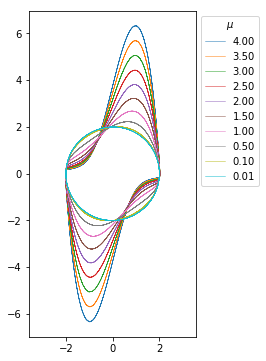
\includegraphics[width=.9\linewidth]{obipy-resources/c515c00ecd6370edf5b32608ff70731e-38847ruq.png}
\end{center}

\subsection{Summary}
\label{sec:orgdcd227e}

Today we covered the conversion of an n\(^{\text{th}}\) order differential equation into a system of first order differential equations.

We examined the use of the optional argument max\_step to fine tune the solution points returned by the solver.

This concludes our the first section on ordinary differential equations.

On Wed, I will answer questions for about half of the class, and we will have a quiz on the second half of class. The quiz will be a single question, and will be representative of the exam next week.

\section{place holder for 06-review?}
\label{sec:org2561016}

\section{07 Nonlinear algebra}
\label{sec:org6852a6e}

\subsection{Introduction to nonlinear algebra}
\label{sec:org0570097}

In non-linear algebra, we seek solutions to the equation \(f(x) = 0\) where \(f(x)\) is \emph{non-linear} in \(x\). These are examples of non-linear algebraic equations:

\begin{itemize}
\item \(e^x=4\)
\item \(x^2 + x - 1 = 0\)
\item \(f(F_A) = F_{A0} - F_{A} - k F_A^2 / \nu / V = 0\)
\end{itemize}

There is not a general theory for whether there is a solution, multiple solutions, or no solution to nonlinear algebraic equations. For example,

\(sin(x) = 2\) has no solution. We define \(f(x) = sin(x) - 2\) and plot it. You can see there no intersections with the x-axis at y=0, meaning no solutions

\begin{minted}[frame=lines,fontsize=\scriptsize,linenos]{ipython}
%matplotlib inline
import matplotlib.pyplot as plt
import numpy as np

x = np.linspace(0, 10)

def f(x):
    return np.sin(x) - 2

plt.plot(x, f(x))
plt.axhline(0, ls='--')
plt.xlabel('x')
plt.ylabel('y')
\end{minted}

\begin{center}
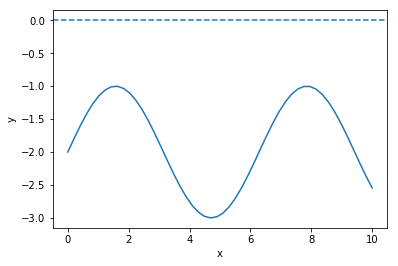
\includegraphics[width=.9\linewidth]{obipy-resources/a42b059ba3fd2f94b3a34f1c9b427f54-26729hzK.png}
\end{center}

In contrast, \(sin(x) = 0.5\) will have an infinite number of solutions, everywhere the function intersects the x-axis.

\begin{minted}[frame=lines,fontsize=\scriptsize,linenos]{ipython}
def f2(x):
    return np.sin(x) - 0.5

plt.plot(x, f2(x))
plt.axhline(0, ls='--')
plt.xlabel('x')
plt.ylabel('y')
\end{minted}

\begin{center}
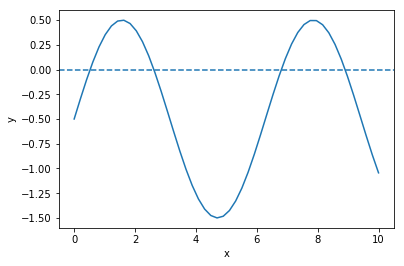
\includegraphics[width=.9\linewidth]{obipy-resources/a42b059ba3fd2f94b3a34f1c9b427f54-26729u9Q.png}
\end{center}

Finally, \(sin(x) = x - 1\) has only one solution.

\begin{minted}[frame=lines,fontsize=\scriptsize,linenos]{ipython}
def f3(x):
    return np.sin(x) - (x - 1)

plt.plot(x, f3(x))
plt.axhline(0, ls='--')
plt.xlabel('x')
plt.ylabel('y')
\end{minted}

\begin{center}
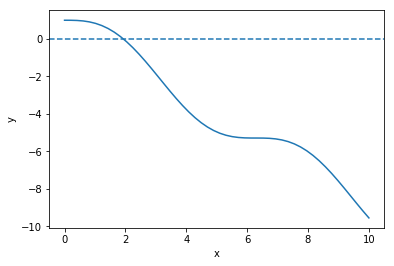
\includegraphics[width=.9\linewidth]{obipy-resources/a42b059ba3fd2f94b3a34f1c9b427f54-267297HX.png}
\end{center}

The equation \(e^{-0.5 x} \sin(x) = 0.5\), evidently has two solutions, but other versions of this equation might have 0, 1, multiple or infinite solutions.

\begin{minted}[frame=lines,fontsize=\scriptsize,linenos]{ipython}
def f3(x):
    return np.exp(-0.5 * x) * np.sin(x) - 0.5

plt.plot(x, f3(x))
plt.axhline(0, ls='--')
plt.title('$e^{-0.5 x} \sin(x) = 0.5$')
plt.xlabel('x')
plt.ylabel('objective')
\end{minted}

\begin{center}
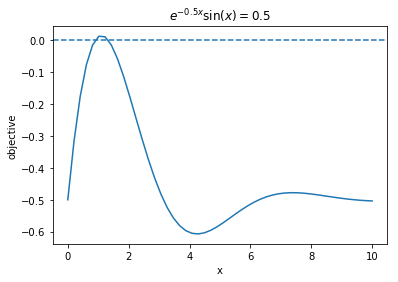
\includegraphics[width=.9\linewidth]{obipy-resources/a42b059ba3fd2f94b3a34f1c9b427f54-26729ISd.png}
\end{center}

\textbf{exercise} modify the equation to see 0, 1, many or infinite solutions.

Graphical methods like this are invaluable to visually assess if there are any solutions, and if so how many solutions at least over some range of solutions. Sometimes, this is the fastest way to estimate a solution. Here we focus on nonlinear algebra problems that cannot be analytically solved. These kinds of problems require an iterative solution approach.

\subsubsection{Newton-Raphson method for finding solutions}
\label{sec:orge8a13fa}

Notes adapted from \url{https://en.wikipedia.org/wiki/Newton\%27s\_method}.

The key idea is that we start with a guess that is close to the solution, and then the function is approximated by a line tangent to the function to find where the line intersects the x-axis. For well-behaved functions, this is a better estimate of where the function equals zero than the first guess. Then, we repeat this until we get sufficiently close to zero.

So, we start with the point (x0, f(x0)), and we compute f'(x0), which is the slope of the line tangent to f(x0). We can express an equation for this line as: \(y - f(x0) = f'(x0)(x - x0)\) If we now solve this for the \(x\) where \(y=0\) leads to:

\(0 = f'(x0)(x - x0) + f(x0)\)

which leads to

\(x = x0 - f(x0) / f'(x0)\)

To implement this, we need to decide what is the tolerance for defining 0, and what is the maximum number of iterations we want to consider?

We will first consider what is the square root of 612? This is equivalent to finding a solution to \(x^2 = 612\)

\(f(x) = x^2 - 612\)

Let's start with a guess of x=25, since we know \(x^2=625\). We also know \(f'(x) = 2x\).

The approach is iterative, so we will specify the maximum number of steps to iterate to, and a criteria for stopping.

\begin{minted}[frame=lines,fontsize=\scriptsize,linenos]{ipython}
x0 = 25

Nmax = 25  # stop if we hit this many iterations
TOL = 1e-3 # stop if we are less than this number

def f(x):
    "The function to solve."
    return x**2 - 612

def fprime(x):
    "Derivative of the function to solve."
    return 2 * x

# Here is the iterative solution
for i in range(Nmax):
    xnew = x0 - f(x0) / fprime(x0)
    x0 = xnew

    print(f'{i}: {xnew}')
    if np.abs(f(xnew)) < TOL:
        break

    if i == Nmax - 1:
        print('Max iterations exceeded')
        break

print(xnew, xnew**2)
\end{minted}

\begin{verbatim}
0: 24.74
1: 24.738633791430882
24.738633791430882 612.0000018665258

\end{verbatim}

That is pretty remarkable, it only took two iterations. That is partly because we started pretty close to the answer. Try this again with different initial guesses and see how the number of iterations changes. Also try with negative numbers. There are two solutions that are possible, and the one you get depends on the initial guess.

One reason it takes so few iterations here is that Newton's method converges quadratically when you are close to the solution, and in this simple case we have a quadratic function, so we get to the answer in just a few steps.

\subsubsection{Problem problems}
\label{sec:org61551ad}

There are pathological situations you can get into. Consider this simple looking polynomial:

\begin{minted}[frame=lines,fontsize=\scriptsize,linenos]{ipython}
def f(x):
    return x**3 - 2 * x + 2

def fprime(x):
    return 3 * x**2 - 2

x = np.linspace(-2, 2)
plt.plot(x, f(x))
plt.xlabel('x')
plt.ylabel('f(x)')
\end{minted}

\begin{center}
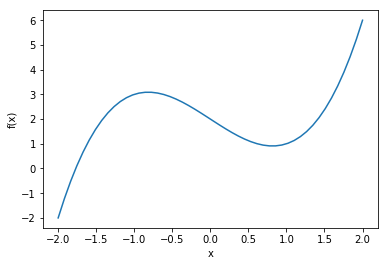
\includegraphics[width=.9\linewidth]{obipy-resources/a42b059ba3fd2f94b3a34f1c9b427f54-26729HKi.png}
\end{center}

It seems obvious there is a root near -1.7. But if you use a guess around x=0, the algorithm simply oscillates back and forth and never converges. Let's see:

\begin{minted}[frame=lines,fontsize=\scriptsize,linenos]{ipython}
x0 = 0

for i in range(Nmax):
    xnew = x0 - f(x0) / fprime(x0)
    x0 = xnew
    print(f'{i}: {xnew}')
    if np.abs(f(xnew)) < TOL:
        break

    if i == Nmax - 1:
        print('Max iterations exceeded')
        break

print(xnew)
\end{minted}

\begin{verbatim}
0: 1.0
1: 0.0
2: 1.0
3: 0.0
4: 1.0
5: 0.0
6: 1.0
7: 0.0
8: 1.0
9: 0.0
10: 1.0
11: 0.0
12: 1.0
13: 0.0
14: 1.0
15: 0.0
16: 1.0
17: 0.0
18: 1.0
19: 0.0
20: 1.0
21: 0.0
22: 1.0
23: 0.0
24: 1.0
Max iterations exceeded
1.0

\end{verbatim}

\textbf{Exercise:} Try several initial guesses, and see which ones converge.


You can also run into problems when:

\begin{itemize}
\item \(f'(x) = 0\) at the initial guess, or a subsequent unpdate, then you get a singularity in the update.
\item The first derivative is discontinuous at the root. Then you may not converge because the update can bounce back and forth.
\item The first derivative is undefined at the root
\end{itemize}

We do not frequently run into these issues, but they do occur from time to time. The solution is usually to use a better initial guess.

\subsection{Derivatives of functions}
\label{sec:org373cedf}

When you can derive an analytical derivative, you should probably consider doing that, because otherwise we have to approximate the derivatives numerically, which is less accurate and computationally more expensive.

Let's examine the \texttt{scipy.misc.derivative} function. You provide a function, an x-value that you want the derivative at, and a dx to use in a finite-difference formula. By default, three points are used in the difference formula. You want to use a small dx to get an accurate result, but not too small or you can get numerical errors.

\textbf{exercise}: Try this out with different values of dx from 0.1 to 1e-15.

\begin{minted}[frame=lines,fontsize=\scriptsize,linenos]{ipython}
from scipy.misc import derivative

def f(x):
    return x**3

x0 = 12

derivative(f, x0, dx=1e-3), 3 * x0**2  # the numerical and analytical derivative
\end{minted}

\begin{verbatim}
(432.00000099977842, 432)
\end{verbatim}

It would be nice to have some adaptive code that just does the right thing to find a dx adaptively. Here is an example:

\begin{minted}[frame=lines,fontsize=\scriptsize,linenos]{ipython}
def fprime(func, x0, dx=0.1, tolerance=1e-6, nmax=10):
    """Estimate the derivative of func at x0. dx is the initial spacing to use, and
    it will be adaptively made smaller to get the derivative accurately with a
    tolerance. nmax is the maximum number of divisions to make.

    """
    d0 = derivative(func, x0, dx=dx)
    for i in range(nmax):
        dx = dx / 2
        dnew = derivative(func, x0, dx=dx)
        if np.abs(d0 - dnew) <= tolerance:
            return dnew
        else:
            d0 = dnew

    # You only get here when the loop has completed and not returned a value
    print('Maximum number of divisions reached')
    return None
\end{minted}

And, here is our derivative function in action:

\begin{minted}[frame=lines,fontsize=\scriptsize,linenos]{ipython}
def f(x):
    return x**3

fprime(f, 12)
\end{minted}

\begin{verbatim}
432.00000015203841
\end{verbatim}

Let's wrap the Newton method in a function too, using our fprime function to get the derivative.

\begin{minted}[frame=lines,fontsize=\scriptsize,linenos]{ipython}
def newton(func, x0, tolerance=1e-6, nmax=10):
    for i in range(nmax):
        xnew = x0 - func(x0) / fprime(func, x0)
        x0 = xnew
        if np.abs(func(xnew)) < tolerance:
            return xnew

    print('Max iterations exceeded')
    return None
\end{minted}

Now, we have a pretty convenient way to solve equations:

\begin{minted}[frame=lines,fontsize=\scriptsize,linenos]{ipython}
def f(x):
    return x**2 - 612

newton(f, 25), np.sqrt(612)
\end{minted}

\begin{verbatim}
(24.738633753705965, 24.738633753705962)
\end{verbatim}

This is the basic idea behind nonlinear algebra solvers. Similar to the ode solver we used, there are functions in scipy written to solve nonlinear equations. We consider these next.

\subsection{fsolve}
\label{sec:org31e9ac6}

\texttt{scipy.optimize.fsolve} is the main function we will use to solve nonlinear algebra problems. \texttt{fsolve} can be used with functions where you have the derivative, and where you don't.

\begin{minted}[frame=lines,fontsize=\scriptsize,linenos]{ipython}
from scipy.optimize import fsolve
?fsolve
\end{minted}

Let's see the simplest example.

Solve \(e^x = 2\).

\begin{minted}[frame=lines,fontsize=\scriptsize,linenos]{ipython}
import numpy as np

def objective(x):
    return np.exp(x) - 2  # equal to zero at the solution

fsolve(objective, 2), np.log(2)
\end{minted}

\begin{verbatim}
(array([ 0.69314718]), 0.69314718055994529)
\end{verbatim}

Note that the result is an array. We can \emph{unpack} the array with this syntax. Note the comma. Why a comma? it indicates to Python that the results should be unpacked into the variable in a special way, i.e. the first value of the result goes into the first variable. That is all there is in this case.

This is the preferred way to get the value of the solution into x:

\begin{minted}[frame=lines,fontsize=\scriptsize,linenos]{ipython}
x, = fsolve(objective, 2)
x
\end{minted}

\begin{verbatim}
0.69314718055994562
\end{verbatim}

Here are two checks on the answer.

\begin{minted}[frame=lines,fontsize=\scriptsize,linenos]{ipython}
objective(x), x - np.log(2)
\end{minted}

\begin{verbatim}
(4.4408920985006262e-16, 3.3306690738754696e-16)
\end{verbatim}

You can get a lot more information by setting full output to 1. Note you have to assign 4 variables to the output in this case. That status will be 1 if it succeeds.

\begin{minted}[frame=lines,fontsize=\scriptsize,linenos]{ipython}
ans, info, status, msg = fsolve(objective, 2, full_output=1)
ans, info, status, msg
\end{minted}

\begin{verbatim}
(array([ 0.69314718]),
 {'fjac': array([[-1.]]),
  'fvec': array([  4.44089210e-16]),
  'nfev': 10,
  'qtf': array([ -4.74712714e-10]),
  'r': array([-2.00000148])},
 1,
 'The solution converged.')
\end{verbatim}

Here is an example with no solution, and a different status flag.

\begin{minted}[frame=lines,fontsize=\scriptsize,linenos]{ipython}
def objective2(x):
    return np.exp(x) + 2

fsolve(objective2, 2, full_output=1)
\end{minted}

\begin{verbatim}
(array([-28.0696978]),
 {'fjac': array([[ 1.]]),
  'fvec': array([ 2.]),
  'nfev': 20,
  'qtf': array([ 2.]),
  'r': array([  6.75011061e-13])},
 5,
 'The iteration is not making good progress, as measured by the \n  improvement from the last ten iterations.')
\end{verbatim}

\subsection{A worked example}
\label{sec:orgbc207c5}

We can integrate fsolve with a variety of other problems. For example, here is an integral equation we need to solve in engineering problems. The volume of a plug flow reactor can be defined by this equation: \(V = \int_{Fa(V=0)}^{Fa} \frac{1}{r_a} dFa\) where \(r_a\) is the rate law. Suppose we know the reactor volume is 100 L, the inlet concentration of A is 1 mol/L, the volumetric flow is 10 L/min, and \(r_a = -k Ca\), with \(k=0.23\) 1/min. What is the exit molar flow rate? We need to solve the following equation:

$$100 = \int_{Fa(V=0)}^{Fa} \frac{1}{-k Fa/\nu} dFa$$

The equation to solve here is:

\(f(Fa) = 100 - \int_{Fa(V=0)}^{Fa} \frac{1}{-k Fa/\nu} dFa\).

\begin{minted}[frame=lines,fontsize=\scriptsize,linenos]{ipython}
import numpy as np
from scipy.integrate import quad
from scipy.optimize import fsolve

k = 0.23   # 1 / min
nu = 10.0  # L / min
Cao = 1.0  # mol / L
Fa0 = Cao * nu

def integrand(Fa):
    return -1.0 / (k * Fa / nu)

def objective(Fa):
    integral, err = quad(integrand, Fao, Fa)
    return 100.0 - integral
\end{minted}

To make a plot, there is a subtlety. We cannot integrate an array of \(F_A\) values. Previously, we used a for loop to get around this. There is another syntax called \emph{list comprehension} that we can also use:

\begin{minted}[frame=lines,fontsize=\scriptsize,linenos]{ipython}
[objective(fa) for fa in [0.01, 0.1, 1]]
\end{minted}

\begin{verbatim}
[-100.2247906951344, -0.11239534756749947, 100.0]
\end{verbatim}

You can already see the answer must be between 0.1 and 1 because the sign changes between these two values.

\begin{minted}[frame=lines,fontsize=\scriptsize,linenos]{ipython}
import matplotlib.pyplot as plt

fa = np.linspace(0.01, 1)
obj = [objective(f) for f in fa]
plt.plot(f, obj)
plt.xlabel('Molar flow rate (mol/min)')
plt.ylabel('objective')
plt.axhline(0, color='k', linestyle='--')
plt.axvline(0.1, color='k', linestyle='--')
\end{minted}

\begin{center}
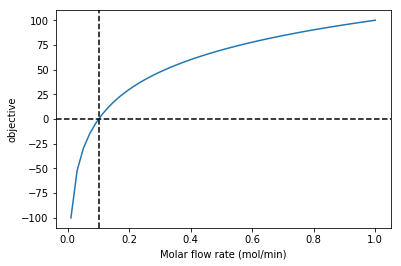
\includegraphics[width=.9\linewidth]{obipy-resources/a42b059ba3fd2f94b3a34f1c9b427f54-26729u2c.png}
\end{center}


You can see there is one answer in this range, near a flow rate of 0.1 mol/min. We use that as an initial guess for fsolve:

\begin{minted}[frame=lines,fontsize=\scriptsize,linenos]{ipython}
Fa_guess = 0.1
Fa_exit, = fsolve(objective, Fa_guess)
print(f'The exit flow rate is {Fa_exit:1.4f} mol/min.')
\end{minted}

\begin{verbatim}
The exit flow rate is 0.1003 mol/min.

\end{verbatim}

\subsection{Parameterized objective functions}
\label{sec:org5014151}

Now, suppose we want to see how our solution varies with a parameter value. For example, we can change the rate constant by changing the temperature. Say we want to compute the exit molar flow rate at a range of rate constants, e.g. from 0.02 to 2 1/min. In other words, we treat the rate constant as a \emph{parameter} and use it in an additional argument.

\begin{minted}[frame=lines,fontsize=\scriptsize,linenos]{ipython}
def integrand(Fa, k):
    return -1.0 / (k * Fa / nu)

def objective(Fa, k):
    integral, err = quad(integrand, Fao, Fa, args=(k,))
    return 100.0 - integral

KRANGE = np.linspace(0.02, 2)

fa_exit = np.zeros(KRANGE.shape)

guess = 0.1

for i, k in enumerate(KRANGE):
    ans, info, status, msg = fsolve(objective, guess, args=(k,), full_output=1)
    if status == 1:
        fa_exit[i] = ans
        guess = ans
    else:
        print(f'k = {k} failed. {msg}')

plt.plot(KRANGE, (Fa0 - fa_exit) / Fa0)
plt.xlabel('k (1/min)')
plt.ylabel('Conversion')
\end{minted}

\begin{center}
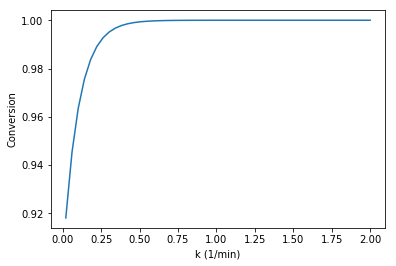
\includegraphics[width=.9\linewidth]{obipy-resources/a42b059ba3fd2f94b3a34f1c9b427f54-26729VVv.png}
\end{center}

You can see here that any rate constant above about 0.5 1/min leads to near complete conversion, so heating above the temperature required for this would be wasteful.


\subsection{Summary}
\label{sec:org192b006}

In this lecture we reviewed methods to solve non-linear algebraic equations (they also work on linear algebra, but it is considered wasteful since there are more efficient methods to solve those).

\begin{itemize}
\item The key idea is to create a function that is equal to zero at the solution, and then use \texttt{scipy.optimize.fsolve} with an initial guess to find the solution.
\item We introduced \emph{list comprehension} which is a convenient syntax for for loops.
\item We also looked at \texttt{scipy.misc.derivative} which is a convenient way to numerically estimate the derivative of a function by finite difference formulas. It is a \emph{function analog} of \texttt{numpy.gradient} which provides derivatives of \emph{data}.
\end{itemize}

Next time, we will generalize this to multiple, coupled nonlinear equations with multiple variables.

\section{08 Nonlinear algebra - coupled equations}
\label{sec:org25e1080}


\subsection{Special nonlinear systems - polynomials}
\label{sec:orgc4564a2}

Polynomials are a special class of nonlinear algebraic equations that are especially easy to solve. A polynomial is linear in the coefficients in front of the variable. If we consider the following \(n^{th}\) order polynomial:

\(p_0 x^n + p_1 x^{(n-1)} + ... + p_{n-1} x + p_n = 0\)

Let's be specific:

\(x^2 + 8x + 16 = 0\)

We express this as [1, 8, 16].

\begin{minted}[frame=lines,fontsize=\scriptsize,linenos]{ipython}
import numpy as np

p = [1, 8, 16]
r = np.roots(p)
r
\end{minted}

\begin{verbatim}
array([-4., -4.])
\end{verbatim}

Note we get all the roots. We can check that with the \texttt{numpy.polyval} command.

\begin{minted}[frame=lines,fontsize=\scriptsize,linenos]{ipython}
np.polyval(p, r)
\end{minted}

\begin{verbatim}
array([ 0.,  0.])
\end{verbatim}

We can also use this to plot a polynomial.

\begin{minted}[frame=lines,fontsize=\scriptsize,linenos]{ipython}
import numpy as np

x = np.linspace(-5, -3)
y = np.polyval(p, x)

%matplotlib inline
import matplotlib.pyplot as plt
plt.plot(x, y)
plt.xlabel('x')
plt.ylabel('y')
\end{minted}







\begin{center}
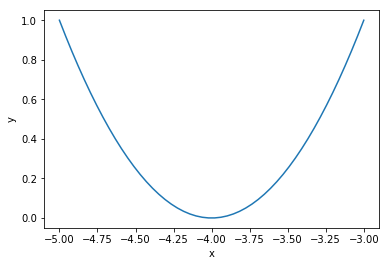
\includegraphics[width=.9\linewidth]{obipy-resources/2cebf4017bd84c109f67e80d93d1304b-17111_sX.png}
\end{center}

Why is this so convenient?

\subsubsection{Cubic equations of state}
\label{sec:org2fa9a0c}

There are applications of polynomials in thermodynamics. The van der waal equation is a cubic polynomial \(f(V) = V^3 - \frac{p n b + n R T}{p} V^2 + \frac{n^2 a}{p}V - \frac{n^3 a b}{p} = 0\), where \(a\) and \(b\) are constants, \(p\) is the pressure, \(R\) is the gas constant, \(T\) is an absolute temperature and \(n\) is the number of moles. The roots of this equation tell you the volume of the gas at those conditions.

\begin{minted}[frame=lines,fontsize=\scriptsize,linenos]{ipython}
# numerical values of the constants
a = 3.49e4
b = 1.45
p = 679.7   # pressure in psi
T = 683     # T in Rankine
n = 1.136   # lb-moles
R = 10.73   # ft^3 * psi / R / lb-mol

ppar = [1.0,
        -(p * n * b + n * R * T) / p,
        n**2 * a / p,
        -n**3 * a * b / p]

print(np.roots(ppar))
\end{minted}

\begin{verbatim}
[ 5.09432376+0.j          4.40066810+1.43502848j  4.40066810-1.43502848j]

\end{verbatim}

Note that only one root is real (and even then, we have to interpret 0.j as not being imaginary. Also, in a cubic polynomial, there can only be two imaginary roots). In this case that means there is only one phase present.

\subsubsection{Other useful things to remember about polynomials}
\label{sec:org6cae4a5}

You can easily get the parameters of the derivative of the polynomial with \texttt{numpy.polyder}.

\begin{minted}[frame=lines,fontsize=\scriptsize,linenos]{ipython}
p = [1, 8, 16]

pd = np.polyder(p)
pd
\end{minted}

\begin{verbatim}
array([2, 8])
\end{verbatim}

You can use these with \texttt{numpy.polyval} to compute the derivative at different points.

\begin{minted}[frame=lines,fontsize=\scriptsize,linenos]{ipython}
np.polyval(pd, 0)
\end{minted}

\begin{verbatim}
8
\end{verbatim}

You can also get the coefficients of the integral of the polynomial. The integration constant is assumed to be 0 by default.

\begin{minted}[frame=lines,fontsize=\scriptsize,linenos]{ipython}
pint = np.polyint(p)
pint
\end{minted}

\begin{verbatim}
array([  0.33333333,   4.        ,  16.        ,   0.        ])
\end{verbatim}

You can use this to compute definite integrals, e.g. from x=1 to x=2:

\begin{minted}[frame=lines,fontsize=\scriptsize,linenos]{ipython}
np.polyval(pint, 2) - np.polyval(pint, 1)
\end{minted}

\begin{verbatim}
30.333333333333339
\end{verbatim}

\textbf{exercise} Use another method to confirm the result above.

Finally, the syntax \texttt{np.polyval(pint, 2)} can be a little tedious. You can create a function with \texttt{numpy.poly1d} using the array of coefficients. Conveniently, you can use the function in the roots, polyder and polyint commands!

\begin{minted}[frame=lines,fontsize=\scriptsize,linenos]{ipython}
p = np.poly1d(pint)
p(2) - p(1)
\end{minted}

\begin{verbatim}
30.333333333333339
\end{verbatim}

\begin{minted}[frame=lines,fontsize=\scriptsize,linenos]{ipython}
np.roots(p)
\end{minted}

\begin{verbatim}
array([-6.+3.46410162j, -6.-3.46410162j,  0.+0.j        ])
\end{verbatim}


\subsection{Systems of nonlinear equations}
\label{sec:orgfc4bb54}

Analogously to systems of ordinary differential equations, with systems of nonlinear equations we define functions that will return a zero for each equation in the system. Then we have to pass an initial guess for each variable to fsolve, and it will return an array of values, one for each variable.

It is considerably more difficult to visualize systems of nonlinear equations. With two equations and two unknowns it is sometimes easy to plot solutions, but not always.

\begin{align}
y &=& x^2 \\
y &=& 8 - x^2
\end{align}

One approach to visualizing this is to plot the two curves.

\begin{minted}[frame=lines,fontsize=\scriptsize,linenos]{ipython}
import numpy as np
%matplotlib inline
import matplotlib.pyplot as plt

x = np.linspace(0, 4)

y1 = x**2
y2 = 8 - x**2

plt.plot(x, y1, x, y2)
plt.xlabel('x')
plt.ylabel('y')
plt.legend(['y1', 'y2'])
\end{minted}

\begin{center}
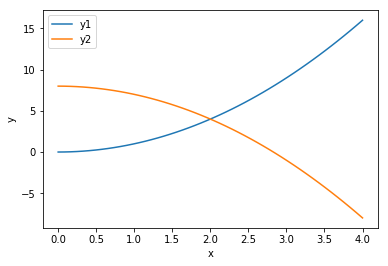
\includegraphics[width=.9\linewidth]{obipy-resources/2cebf4017bd84c109f67e80d93d1304b-26729kvr.png}
\end{center}

You can see that on this domain, there is one place where the two curves intersect near the point (2, 5), which is a solution point. At this point there is one (x, y) pair that is a solution to \emph{both} equations.

\begin{minted}[frame=lines,fontsize=\scriptsize,linenos]{ipython}
from scipy.optimize import fsolve

def objective(X):
    x, y = X
    z1 = y - x**2
    z2 = y - 8 + x**2
    return np.array([z1, z2])

guess = [2, 5]
fsolve(objective, guess)
\end{minted}

\begin{verbatim}
array([ 2.,  4.])
\end{verbatim}

It is not always easy to solve for one variable in terms of the other though. In that case, we can resort to an alternate graphical approach where we evaluate the objective function over a range of the variables, and look for regions where they overlap.

Consider the solution to these equations (adapted from \url{https://www.mathworks.com/help/optim/ug/fsolve.html}):

\(e^{-e^{-(x_1 + x_2)}} = x_2 (1 + x_1^2)\)

and

\(x_1 \cos(x_2) + x_2 \sin(x_1) = 1/2\)

It is not possible to solve either one for one variable in terms of the other. So instead, we will compute the objective function for a range of \(x_1, x_2\) values, and then use a contour plot of each equation to see where there might be a solution.

The key to this visualization is where we draw the contours. A good choice is to highlight only the part of the solutions that bracket zero. Then we can see where they intersect, because there is probably a solution in that neighborhood.

\begin{minted}[frame=lines,fontsize=\scriptsize,linenos]{ipython}
def objective(X):
    x1, x2 = X
    z1 = np.exp(-np.exp(-(x1 + x2))) - x2 * (1 + x1**2)
    z2 = x1 * np.cos(x2) + x2 * np.sin(x1) - 0.5
    return np.array([z1, z2])


x1 = np.linspace(0, 1)
x2 = np.linspace(0, 1)

X1, X2 = np.meshgrid(x1, x2)

Z1, Z2 = objective([X1, X2])

plt.contour(X1, X2, Z1, levels=np.linspace(-0.1, 0.1, 100))
plt.contour(X1, X2, Z2, levels=np.linspace(-0.1, 0.1, 100))
plt.xlabel('$x_1$')
plt.ylabel('$x_2$')
plt.colorbar()
\end{minted}

\begin{center}
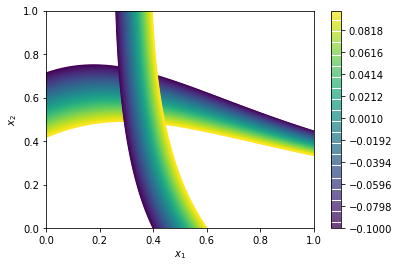
\includegraphics[width=.9\linewidth]{obipy-resources/2cebf4017bd84c109f67e80d93d1304b-26729XzN.png}
\end{center}

There is an intersection near \(x_1=0.4\), and \$x\_2 = 0.6. We can use that as an initial guess.

\begin{minted}[frame=lines,fontsize=\scriptsize,linenos]{ipython}
ans = fsolve(objective, [0.4, 0.6])  # note we do not need ans, because ans will have two values in it.
ans, objective(ans)
\end{minted}

\begin{verbatim}
(array([ 0.35324662,  0.60608174]),
 array([ -2.22044605e-16,   1.11022302e-16]))
\end{verbatim}

This shows the solution, and that the objective is practically equal to zero at that point.

You can see that trying to do this in more than 2 dimensions can quickly get difficult to visualize!

\subsection{Summary}
\label{sec:org4b6521a}

\begin{itemize}
\item We learned about a special class of nonlinear functions that are polynomials, and a series of useful functions to manipulate them.

\item We learned that you can use fsolve to find solutions to coupled non-linear algebraic equations.

\item Next time, we will apply this to solving a nonlinear boundary value differential equation.
\end{itemize}

\section{09 Solving nonlinear BVPs by finite differences}
\label{sec:org136131a}

Adapted from Example 8.7 in \uline{Numerical Methods in Engineering with Python} by Jaan Kiusalaas.

We want to solve \(y''(x) = -3 y(x) y'(x)\) with \(y(0) = 0\) and \(y(2) = 1\).

This is a boundary value problem. First we consider using a finite difference method. We discretize the region and approximate the derivatives as:

\(y''(x) \approx \frac{y_{i-1} - 2 y_i + y_{i+1}}{h^2}\)

\(y'(x) \approx \frac{y_{i+1} - y_{i-1}}{2 h}\)

We define a function \(y''(x) = F(x, y, y')\). At each node in our discretized region, we will have an equation that looks like \(y''(x) - F(x, y, y') = 0\), which will be nonlinear in the unknown solution \(y\). The set of equations to solve is:

\begin{eqnarray}
y_0 - \alpha &=& 0 \\
\frac{y_{i-1} - 2 y_i + y_{i+1}}{h^2} + (3 y_i) (\frac{y_{i+1} - y_{i-1}}{2 h}) &=& 0 \\
y_L - \beta &=&0
\end{eqnarray}

Since we use a nonlinear solver, we will have to provide an initial guess to the solution. We will in this case assume a line. In other cases, a bad initial guess may lead to no solution.

\begin{minted}[frame=lines,fontsize=\scriptsize,linenos]{ipython}
import numpy as np
from scipy.optimize import fsolve
%matplotlib inline
import matplotlib.pyplot as plt

x1 = 0.0
x2 = 2.0

alpha = 0.0
beta = 1.0
\end{minted}

We need to specify a grid of points to discretize the solution on. We will start with a small grid because it is easy to visualize, but note that the grid spacing determines how good the approximation to the derivative is, so we will have to return here to see what the impact of our spacing is.

\begin{minted}[frame=lines,fontsize=\scriptsize,linenos]{ipython}
N = 10
X, h = np.linspace(x1, x2, N, retstep=True)
\end{minted}

Now, we can define functions for the differential equation, and for the nonlinear equations.

\begin{minted}[frame=lines,fontsize=\scriptsize,linenos]{ipython}
def residuals(y):
    "When we have the right values of y, this function will be zero."

    res = np.zeros(y.shape) # we need a zero for each node

    res[0] = y[0] - alpha # this is the boundary value y(alpha) = 0

    for i in range(1, N - 1):
        x = X[i]
        # Approximation of y'' from the current point
        YPP = (y[i - 1] - 2 * y[i] + y[i + 1]) / h**2

        # Approximation of y'
        YP = (y[i + 1] - y[i - 1]) / (2 * h)

        # y'' + 3 * y * y' = 0
        res[i] = YPP + 3 * y[i] * YP

    res[-1] = y[-1] - beta # y(beta) = 0
    return res
\end{minted}

We need a guess, and here we guess a line.

\begin{minted}[frame=lines,fontsize=\scriptsize,linenos]{ipython}
# we need an initial guess
init = alpha + (beta - alpha) / (x2 - x1) * X
plt.plot(X, init)
\end{minted}

\begin{verbatim}
[<matplotlib.lines.Line2D at 0x1172b56a0>]
\end{verbatim}



\begin{center}
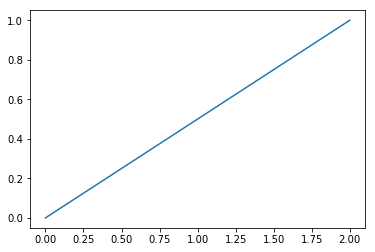
\includegraphics[width=.9\linewidth]{obipy-resources/9f7f3151fe203e2a10edce4b06f0b33f-90490Pwa.png}
\end{center}

We should check our residuals function. We mostly want to see that it runs, and produces the right shaped output.

\begin{minted}[frame=lines,fontsize=\scriptsize,linenos]{ipython}
residuals(init)
\end{minted}

\begin{verbatim}
array([ 0.        ,  0.16666667,  0.33333333,  0.5       ,  0.66666667,
        0.83333333,  1.        ,  1.16666667,  1.33333333,  0.        ])
\end{verbatim}

Now, we solve the BVP.

\begin{minted}[frame=lines,fontsize=\scriptsize,linenos]{ipython}
Y, info, status, msg = fsolve(residuals, init, full_output=1)
print(msg)

plt.plot(X, Y)
plt.xlabel('x')
plt.ylabel('y')
\end{minted}

\begin{verbatim}
The solution converged.

\end{verbatim}




\begin{center}
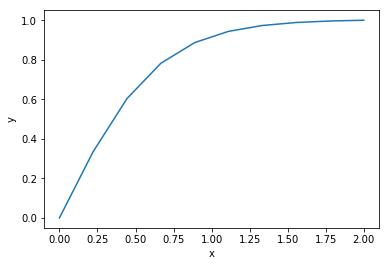
\includegraphics[width=.9\linewidth]{obipy-resources/9f7f3151fe203e2a10edce4b06f0b33f-90490c6g.png}
\end{center}

The solution is jagged because we only used about 10 points. How can you tell if the solution is correct? We can estimate the derivatives, and see how well they fit the equation. We look for:

\(y'' + 3 y y' = 0\) for all \(x\).

\begin{minted}[frame=lines,fontsize=\scriptsize,linenos]{ipython}
yp = np.gradient(Y, X, edge_order=2)
ypp = np.gradient(yp, X, edge_order=2)

plt.plot(X, ypp + 3 * Y * yp)
plt.xlabel('x')
plt.ylabel('residuals')
\end{minted}

\begin{center}
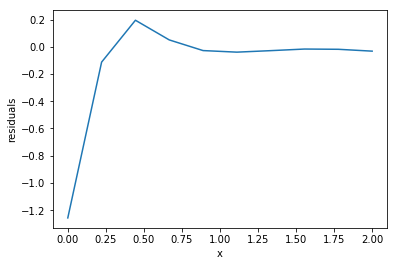
\includegraphics[width=.9\linewidth]{obipy-resources/9f7f3151fe203e2a10edce4b06f0b33f-90490pEn.png}
\end{center}

This result doesn't look great at the origin, but remember:
\begin{enumerate}
\item we used a coarse grid, so the derivative \emph{approximations} are probably not that accurate
\item Numerical derivatives at the end-points are less accurate than in the middle.
\end{enumerate}

\textbf{exercise} Go back and repeat this for a finer grid, e.g. with 50, 100 points.

The approach described here is pretty general. Here, we were able to solve a second-order BVP by discretizing it, approximating the derivatives at the points, and solving the corresponding nonlinear algebra equations. This approach can be extended in a variety of ways, including to systems of equations, and to 2D or 3D systems (where this approach is called finite-element). You will see these kinds of problems extensively in the spring semster in the Transport class.

As we have seen before, however, there are functions in \texttt{scipy} that can help solve these problems.

\subsection{Introduction to solve\_bvp}
\label{sec:orgbbc6ea6}

\begin{minted}[frame=lines,fontsize=\scriptsize,linenos]{ipython}
from scipy.integrate import solve_bvp

solve_bvp?
\end{minted}

\subsubsection{A worked bvp problem}
\label{sec:org63f52bd}

In the pressure driven flow of a fluid with viscosity \(\mu\) between two stationary plates separated by distance \(d\) and driven by a pressure drop \(\Delta P/\Delta x\), the governing equations on the velocity \(u\) of the fluid are (assuming flow in the x-direction with the velocity varying only in the y-direction):

$$\frac{\Delta P}{\Delta x} = \mu \frac{d^2u}{dy^2}$$

with boundary conditions \(u(y=0) = 0\) and \(u(y=d) = 0\), i.e. the no-slip condition at the edges of the plate.

we convert this second order BVP to a system of ODEs by letting \(u_1 = u\), \(u_2 = u_1'\) and then \(u_2' = u_1''\). This leads to:

\(\frac{d u_1}{dy} = u_2\)

\(\frac{d u_2}{dy} = \frac{1}{\mu}\frac{\Delta P}{\Delta x}\)

with boundary conditions \(u_1(y=0) = 0\) and \(u_1(y=d) = 0\).

for this problem we let the plate separation be d=0.1, the viscosity \(\mu = 1\), and \(\frac{\Delta P}{\Delta x} = -100\).


\begin{minted}[frame=lines,fontsize=\scriptsize,linenos]{ipython}
import numpy as np

d = 0.1
mu = 1
deltaPdeltax = -100
\end{minted}

The function defining the BVP has to return an array that has a row for each equation, and a column for each value in the grid.

\begin{minted}[frame=lines,fontsize=\scriptsize,linenos]{ipython}
def bvp(y, U):
    u1, u2 = U
    du1dy = u2
    du2dy = np.ones(y.shape) / mu * deltaPdeltax
    return [du1dy, du2dy]
\end{minted}

The boundary condition function will get the whole numeric solution at each boundary. We want \(u1(a) = 0\) and \(u1(b)=0\).

\begin{minted}[frame=lines,fontsize=\scriptsize,linenos]{ipython}
def bc(Ua, Ub):
    u1a, u2a = Ua
    u1b, u2b = Ub
    return [u1a, u1b]
\end{minted}

Next, we need an initial guess for u1 and u2 on a grid of points. You have to make some decisions here. You need a guess that is reasonably close, but not hard to construct. Here, we anticipate a solution that looks parabolic, and that goes through the points: (0, 0), (d, 0), and some point at (d / 2, ?), where ? represents the point of maximum velocity in middle. We can easily get this polynomial with np.polyfit.

We don't know what the maximum velocity is, so we make a guess, say 0.5. Then, we get the parameters, and apply them to an array of y values.

\begin{minted}[frame=lines,fontsize=\scriptsize,linenos]{ipython}
pars = np.polyfit([0, d / 2, d], [0, 0.5, 0], 2)
pars
\end{minted}

\begin{verbatim}
array([ -2.00000000e+02,   2.00000000e+01,  -4.48803257e-16])
\end{verbatim}

Now, we can define a Y grid and define the guess for the first U1.

\begin{minted}[frame=lines,fontsize=\scriptsize,linenos]{ipython}
Y = np.linspace(0, d)

U1 = np.polyval(pars, Y)
\end{minted}

We also need a guess for U2, and in this case we know that \(u2 = u1'\), so we just use that.

\begin{minted}[frame=lines,fontsize=\scriptsize,linenos]{ipython}
U2 = np.gradient(U1, Y, edge_order=2)

U = np.array([U1, U2])
print(U.shape)
\end{minted}

\begin{verbatim}
(2, 50)

\end{verbatim}

You should \emph{always} visualize the guess to make sure it does what you want. It is \textbf{hard} to make these!

\begin{minted}[frame=lines,fontsize=\scriptsize,linenos]{ipython}
%matplotlib inline
import matplotlib.pyplot as plt
plt.plot(Y, U[0], label='u1')
plt.gca().tick_params('y', colors='b')
plt.ylabel('u1')

plt.twinx()
plt.plot(Y, U[1], 'r', label='u2')
plt.gca().tick_params('y', colors='r')
plt.ylabel('u2')
plt.legend()
\end{minted}

\begin{center}
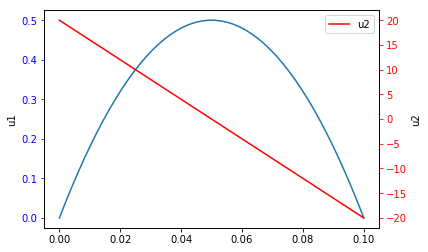
\includegraphics[width=.9\linewidth]{obipy-resources/9f7f3151fe203e2a10edce4b06f0b33f-90490rG1.png}
\end{center}

Now, we are ready to solve the BVP.

\begin{minted}[frame=lines,fontsize=\scriptsize,linenos]{ipython}
from scipy.integrate import solve_bvp

sol = solve_bvp(bvp, bc, Y, U)
print(sol.message)
plt.plot(sol.x, sol.y[0])
plt.xlabel('y')
plt.ylabel('U')
\end{minted}

\begin{verbatim}
The algorithm converged to the desired accuracy.

\end{verbatim}




\begin{center}
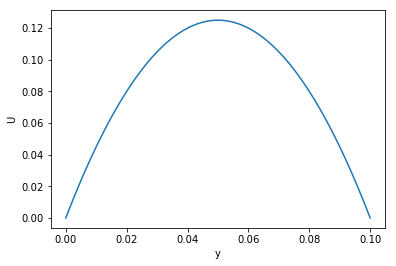
\includegraphics[width=.9\linewidth]{obipy-resources/9f7f3151fe203e2a10edce4b06f0b33f-90490dQE.png}
\end{center}

\textbf{exercise} Try using different guesses, e.g. lines, or triangle shapes, etc. What else looks like this shape? Half a cycle of a sin wave? A semi-circle?

\subsubsection{Concentration profile in a particle}
\label{sec:org2f36a69}

Another typical boundary value problem in chemical engineering is the concentration profile inside a catalyst particle. Here is the dimensionless equation for a second order reaction in a slab. Note here we have a boundary condition on the derivative at the origin. This kind of condition means either there is no flux at this position, or that the slab is symmetric about this position.

\(\frac{d^2c}{dx^2} = \Phi^2 c^2\)

with \(c'(0)\) = 0 and \(c(1) = 1\)

We again convert this to a system of first order differential equations like this:

Let c1 = c, c1' = c', and c2 = c1', so c2' = c1'' = c''

Then we have:

\(c1' = c2\)

\(c2' = \Phi^2 c1^2\)

with boundary conditions \(c1'(0) = 0\) and \(c1(0) = 1\).

We begin with the required functions:

\begin{minted}[frame=lines,fontsize=\scriptsize,linenos]{ipython}
Phi = 50

def bvp(x, C):
    c1, c2 = C
    dc1dx = c2
    dc2dx = Phi**2 * c1**2
    return [dc1dx, dc2dx]

def bc(Ca, Cb):
    c1a, c2a = Ca
    c1b, c2b = Cb

    # Now, evaluate the derivatives at the first boundary condition
    c1prime, c2prime = bvp(0, [c1a, c2a])
    return [c1prime,  # will all equal zero
            c1b - 1]  # c1(b) = 1
\end{minted}

We need an initial guess. We make a naive one, that \(c(x) = 1\) in the slab, i.e. there is no reaction. As usual, we visualize the guess to be sure it does what we intended.

\begin{minted}[frame=lines,fontsize=\scriptsize,linenos]{ipython}
X = np.linspace(0, 1)

C1 = np.ones(X.shape)
C2 = np.gradient(C1, X)

plt.plot(X, C1)
\end{minted}

\begin{verbatim}
[<matplotlib.lines.Line2D at 0x1128ca5c0>]
\end{verbatim}



\begin{center}
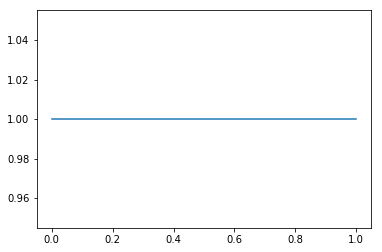
\includegraphics[width=.9\linewidth]{obipy-resources/9f7f3151fe203e2a10edce4b06f0b33f-90490qaK.png}
\end{center}


Now we solve the system.

\begin{minted}[frame=lines,fontsize=\scriptsize,linenos]{ipython}
C = [C1, C2]
sol = solve_bvp(thiele, bc, X, C)
sol.message
\end{minted}

\begin{verbatim}
'The algorithm converged to the desired accuracy.'
\end{verbatim}

\begin{minted}[frame=lines,fontsize=\scriptsize,linenos]{ipython}
plt.plot(sol.x, sol.y[0])
plt.xlabel('x')
plt.ylabel('C')
plt.xlim([0, 1])
plt.ylim([0, 1])
\end{minted}

\begin{verbatim}
(0, 1)
\end{verbatim}



\begin{center}
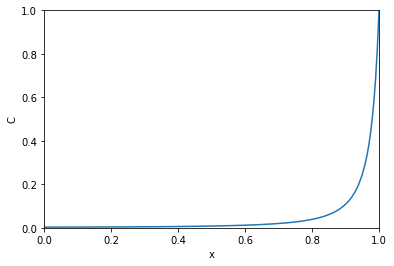
\includegraphics[width=.9\linewidth]{obipy-resources/9f7f3151fe203e2a10edce4b06f0b33f-904903kQ.png}
\end{center}

You can see the solution looks nothing like our initial guess. In this case, a high thiele modulus means most of the reaction happens near the catalyst surface, and the interior of the slab has hardly any reactant in it. This solution is consistent with that.


The effectiveness factor for this system is defined by:

\(E = \int_0^1 c^2 dx\)

We can estimate this with the trapezoid or Simpson's method (remember that the solution is a vector of numbers).

\begin{minted}[frame=lines,fontsize=\scriptsize,linenos]{ipython}
c = sol.y[0]
print(np.trapz(c**2, sol.x))

from scipy.integrate import simps
print(simps(c**2, sol.x))
\end{minted}

\begin{verbatim}
0.016528962861
0.0163346209448

\end{verbatim}

Or, we can use the dense\_output of the solution with quad.

\begin{minted}[frame=lines,fontsize=\scriptsize,linenos]{ipython}
from scipy.integrate import quad

def integrand(x):
    c1, c2 = sol.sol(x)
    return c1**2

quad(integrand, 0, 1)
\end{minted}

\begin{verbatim}
(0.016329985883573546, 9.761482252679577e-09)
\end{verbatim}


\textbf{excercise} Repeat this example for different values of \(\Phi\).

\textbf{exercise} Try different kinds of guesses. Think of a guess that has the properties of the boundary conditions, e.g. c'(0) = 0, and c(1) = 1.

\textbf{exercise} Evaluate the quality of the solution based on the equations.

\subsection{Summary}
\label{sec:org6e14048}

Today, we leveraged the ability to solve systems of nonlinear algebraic equations to solve boundary value problems by discretizing them on a grid, approximating them at the grid points, and then solving the resulting nonlinear equations.

We also learned about the solve\_bvp function, which is in scipy.integrate to solve systems of first-order boundary value problems.

Next time, we will return to nonlinear algebra to see how the algorithms can be used to find minima and maxima.
\section{10Minimization/maximization of functions}
\label{sec:org261ab4a}

\subsection{Function extrema}
\label{sec:org069abc3}

It is pretty common to need to find extreme values of a function in engineering analysis. An extreme value is often a maximum or minimum in a function, and we seek them when we want to maximize a profit function, or minimize a cost function, identify a maximum safe operating condition, etc.

Let's consider an example function with a graphical solution approach. We want a quantitative estimate of the minimum in this function.

\begin{minted}[frame=lines,fontsize=\scriptsize,linenos]{ipython}
import numpy as np
%matplotlib inline
import matplotlib.pyplot as plt

def f(x):
    return x**2 + np.exp(-5 * x**2)

x = np.linspace(0, 2)
y = f(x)
plt.plot(x, y)
\end{minted}

\begin{verbatim}
[<matplotlib.lines.Line2D at 0x110c07c88>]
\end{verbatim}



\begin{center}
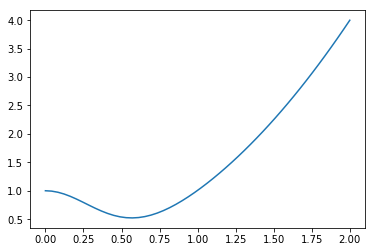
\includegraphics[width=.9\linewidth]{obipy-resources/baab0982fed766ced9ac305dd57e067d-90490fZG.png}
\end{center}

You can see there is a minimum near 0.6. We can find the minimum in a crude kind of way by finding the index of the minimum value in the y-array, and then getting the corresponding value of the x-array. You control the accuracy of this answer by the number of points you discretize the function over.

\begin{minted}[frame=lines,fontsize=\scriptsize,linenos]{ipython}
x = np.linspace(0, 2, 50)
y = f(x)
i = np.argmin(y)
x[i]
\end{minted}

\begin{verbatim}
0.56735044900299336
\end{verbatim}

What are the pros and cons of this method:

Pros:
\begin{enumerate}
\item It is \emph{easy}.
\item You \emph{see} the whole domain you are looking at, and it is easy to see how many extrema their are
\end{enumerate}

Cons:
\begin{enumerate}
\item \emph{Lot's} of function evaluations. Imagine if it took a long time to compute each value.
\item Somewhat tedious.
\item Not so easy to reproduce
\item Not scalable to large problems, your time to do this becomes a limiting factor.
\end{enumerate}

\subsubsection{Find the derivative, and solve for where it is zero}
\label{sec:org0f106f9}

We can also derive the first derivative:

\(y' = 2 * x + e^{-5 x^2} (-10 * x)\)

and solve it for zero using fsolve.

\begin{minted}[frame=lines,fontsize=\scriptsize,linenos]{ipython}
def yp(x):
    return 2 * x + np.exp(-5 * x**2) * (-10 * x)

from scipy.optimize import fsolve
fsolve(yp, 0.5)
\end{minted}

\begin{verbatim}
array([ 0.56735137])
\end{verbatim}

These two answer agree to 5 decimal places.

This depends on your ability to correctly derive and implement the derivative. It is good to know you can solve this problem by more than one method. Here, we use a numerical derivative in the function instead to check our derivative. You can check the convergence of the derivative by varying the dx.

\begin{minted}[frame=lines,fontsize=\scriptsize,linenos]{ipython}
from scipy.misc import derivative

def ypd(x):
    return derivative(f, x, dx=1e-6)

fsolve(ypd, 0.5)
\end{minted}

\begin{verbatim}
array([ 0.56735137])
\end{verbatim}

These look the same within tolerance. This is not a beautiful solution, but it is hard to argue with success here!

\subsubsection{Newton-Raphson method of minima finding}
\label{sec:orgaaff89a}

To use the Newton-Raphson method to get the minimum, we use an iterative approach with:

\(x_{n+1} = x_n - \frac{y'(x_n)}{y''(x_n)}\).

We have to derive these formulas if you want to use analytical derivatives:

\(y' = 2 * x + e^{-5 x^2} (-10 * x)\)

\(y'' = 2 + e^{-5 x^2} (-10 * x)^2 - 10 e^{-5 x^2}\)

Alternatively, we can estimate the derivatives numerically using \texttt{scipy.misc.derivative}. This has the downside of numerical instability for dx that is too small, or low accuracy if it is too large, and the need to check if you made a good choice for it. On the plus side, it avoids making mistakes in the derivative derivation and implementation.

\begin{minted}[frame=lines,fontsize=\scriptsize,linenos]{ipython}
from scipy.misc import derivative

x0 = 0.2
f0 = f(x0)

for i in range(15):
    yp = derivative(f, x0, dx=1e-6, n=1)
    ypp = derivative(f, x0, dx=1e-6, n=2)
    xnew = x0 - yp / ypp
    fnew = f(xnew)

    if np.abs(yp) <= 1e-6:
        break
    x0 = xnew
    f0 = fnew


xnew, fnew, yp, i
\end{minted}

\begin{verbatim}
(0.56735137479655973, 0.5218875824868201, 3.3306690738754696e-10, 5)
\end{verbatim}

This answer also agrees to at least 5 decimal places. This is the gist of what happens in fsolve.

As we have seen many times, finding minima is such a common task that there are dedicated functions available for doing it. One of the is \texttt{scipy.optimize.fmin}. This has a similar signature as \texttt{scipy.optimize.fsolve}, you give it a function and an initial guess, and it iteratively searches for a minimum.

\subsection{scipy.optimize.minimize}
\label{sec:org0bb73c2}

\begin{minted}[frame=lines,fontsize=\scriptsize,linenos]{ipython}
from scipy.optimize import minimize
minimize?
\end{minted}

Here is the basic use of fmin. As always, we should plot the answer where feasible to make sure it is the minimum we wanted.

\begin{minted}[frame=lines,fontsize=\scriptsize,linenos]{ipython}
def f(x):
    return x**2 + np.exp(-5 * x**2)

guess = 0.5
sol = minimize(f, guess)
sol
\end{minted}

\begin{verbatim}
     fun: 0.5218875824868201
hess_inv: array([[ 0.15524504]])
     jac: array([  4.47034836e-08])
 message: 'Optimization terminated successfully.'
    nfev: 15
     nit: 3
    njev: 5
  status: 0
 success: True
       x: array([ 0.56735137])
\end{verbatim}

\begin{minted}[frame=lines,fontsize=\scriptsize,linenos]{ipython}
x = np.linspace(0, 2)
y = f(x)

plt.plot(x, y, 'b-')
plt.plot(sol.x, f(sol.x), 'ro')
plt.xlabel('x')
plt.ylabel('y')
plt.legend(['f(x)', 'fmin'])
\end{minted}

\begin{center}
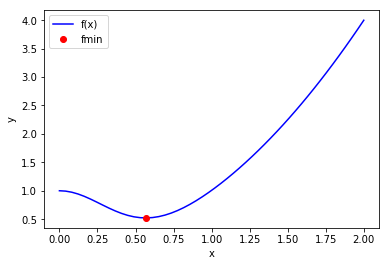
\includegraphics[width=.9\linewidth]{obipy-resources/baab0982fed766ced9ac305dd57e067d-90490HHI.png}
\end{center}

Note this answer is only the same in the first 4 decimal places. Remember that these iterative approaches stop when a tolerance is met. Check the defaults on fmin!

\subsubsection{Multiple minima}
\label{sec:orgc8f8507}

It is possible for functions to have more than one minimum. In this case, your guess will determine which minimum is found. Here is an example where there is a minimum near 2.2, and one near 4.5.

\begin{minted}[frame=lines,fontsize=\scriptsize,linenos]{ipython}
def h(x):
    return 2 + np.cos(x) + np.cos(2*x - 0.5) / 2

x = np.linspace(0, 2 * np.pi)

plt.plot(x, h(x))
plt.xlabel('x')
plt.ylabel('h(x)')
\end{minted}

\begin{center}
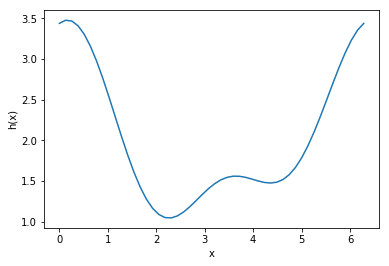
\includegraphics[width=.9\linewidth]{obipy-resources/baab0982fed766ced9ac305dd57e067d-90490hbU.png}
\end{center}

This guess finds the one near 2.2:

\begin{minted}[frame=lines,fontsize=\scriptsize,linenos]{ipython}
minimize(h, 2)
\end{minted}

\begin{verbatim}
     fun: 1.0448871783746694
hess_inv: array([[ 0.52336689]])
     jac: array([ -2.98023224e-08])
 message: 'Optimization terminated successfully.'
    nfev: 15
     nit: 3
    njev: 5
  status: 0
 success: True
       x: array([ 2.26106174])
\end{verbatim}

and this guess finds the one near 4.5

\begin{minted}[frame=lines,fontsize=\scriptsize,linenos]{ipython}
minimize(h, 4)
\end{minted}

\begin{verbatim}
     fun: 1.4758979742813512
hess_inv: array([[ 0.94727664]])
     jac: array([ -9.08970833e-07])
 message: 'Optimization terminated successfully.'
    nfev: 21
     nit: 5
    njev: 7
  status: 0
 success: True
       x: array([ 4.35545599])
\end{verbatim}

You have to decide which one is better for the problem at hand. If this were a cost function, the one at the lower cost is probably better! Note that all we can say here is which one is lower in the interval we are looking at. By inspection of the function, you can see it will be periodic, so there will be many other minima that also exist.

\subsubsection{Finding maxima}
\label{sec:orgfbf6d23}

\texttt{fmin} is for finding \emph{minima}. We can use it to find maxima though, but finding the \emph{minima} of \(-f(x)\). You can see here that when we plot \(-h(x)\) the minima become maxima, and vice-versa. Now you can see there are two definite minima, one near zero, and one near 3.5, which correspond to the maxima of \(h(x)\).

\begin{minted}[frame=lines,fontsize=\scriptsize,linenos]{ipython}
plt.plot(x, -h(x))
plt.xlabel('x')
plt.ylabel('-h(x)')
\end{minted}

\begin{center}
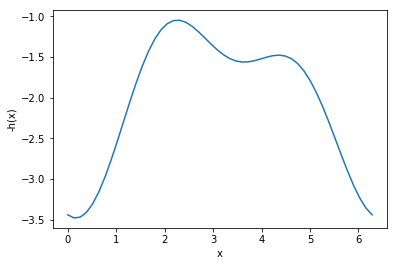
\includegraphics[width=.9\linewidth]{obipy-resources/baab0982fed766ced9ac305dd57e067d-90490ula.png}
\end{center}

The standard way to use fmin is to define an optional argument for the sign that defaults to one. Then, when we call fmin, we will pass -1 as the sign to the function, so we find the minimum of -h(x). Then, we evaluate h(x) at that x-value to get the actual value of the maximum. It is not necessary do this, you can also manually pass around the sign and try to keep it straight.

Here is an example to find the maximum near 3.5.

\begin{minted}[frame=lines,fontsize=\scriptsize,linenos]{ipython}
def h(x, sign=1):
    return sign * (2 + np.cos(x) + np.cos(2*x - 0.5) / 2)

sol = minimize(h, 3.5, args=(-1,))  # set sign=-1 here to minimize -h(x)
print(h(sol.x))  # sign defaults to 1 here, so we get the maximum value

plt.plot(x, h(x))
plt.plot(sol.x, h(sol.x), 'ro')
plt.xlabel('x')
plt.ylabel('h(x)')
\end{minted}

\begin{verbatim}
[ 1.56120872]

\end{verbatim}




\begin{center}
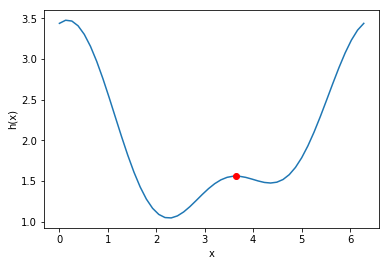
\includegraphics[width=.9\linewidth]{obipy-resources/baab0982fed766ced9ac305dd57e067d-904907vg.png}
\end{center}

Once again, here you have to decide which maximum is relevant

\subsubsection{Application to maximizing profit in a PFR}
\label{sec:orgd24c437}

Compound X with concentration of \(C_{X0} = 2.5\) kmol / m\(^{\text{3}}\) at a flow rate of 12 m\(^{\text{3}}\)/min is converted to Y in a first order reaction with a rate constant of 30 1/min in a tubular reactor. The value of Y is \$1.5/kmol. The cost of operation is \$2.50 per minute per m\(^{\text{3}}\). Find the reactor length that maximizes the profit (profit is value of products minus operating costs).

First, consider why there is a maximum. At low volumes the operating cost is low, and the production of Y is low. At high volumes, you maximize production of Y, so you have the most value, but the operating costs go up (to infinity for complete conversion!). Somewhere in the middle is where a maximum is.

Here are some relevant constants.

\begin{minted}[frame=lines,fontsize=\scriptsize,linenos]{ipython}
cost = 2.5  # dollar/min/m**3
y_value  = 1.5 # dollar / mol

Cx0 = 2.5 # kmol / m**3
v0 = 12.0 # m**3 / min

k = 30.0 # 1/min
\end{minted}

To compute the profit as a function of reactor volume, we need to compute how much Y is produced, then multiply that by the value of Y and subtract the operating cost. To compute how much Y is produced, we use a mole balance on X and Y, and integrate it to the volume to get the molar flows of X and Y. I like to write mole balances like this.

\begin{minted}[frame=lines,fontsize=\scriptsize,linenos]{ipython}
def dFdV(V, F):
    'PFR mole balances on X and Y.'
    Fx, Fy = F
    Cx = Fx / v0
    rx = -k * Cx
    ry = -rx

    dFdX = rx
    dFdY = ry
    return [dFdX, dFdY]

F0 = [Cx0 * v0,  # Fx0
      0.0]       # Fy0
\end{minted}

Now, we can write a profit function. It will take a V as the argument, integrate the PFR to that volume to find the molar exit flow rates, and then compute the profit.

\begin{minted}[frame=lines,fontsize=\scriptsize,linenos]{ipython}
import numpy as np
from scipy.integrate import solve_ivp

def profit(V, sign=1):
    Vspan = (0, V)
    sol = solve_ivp(dFdV, Vspan, F0)
    Fx, Fy = sol.y
    Fy_exit = Fy[-1]
    return sign * (Fy_exit * y_value - cost * V)
\end{minted}

It is always a good idea to plot the profit function. We use a list comprehension here because the profit function is not \emph{vectorized}, which means we cannot pass an array of volumes in and get an array of profits out.

\begin{minted}[frame=lines,fontsize=\scriptsize,linenos]{ipython}
Vspan = np.linspace(0, 4)
profit_array = [profit(V) for V in Vspan]

%matplotlib inline
import matplotlib.pyplot as plt
plt.plot(Vspan, profit_array)
plt.xlabel('V')
plt.ylabel('profit')
\end{minted}

\begin{center}
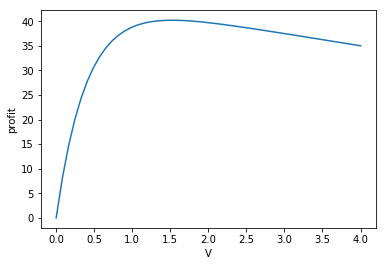
\includegraphics[width=.9\linewidth]{obipy-resources/baab0982fed766ced9ac305dd57e067d-90490I6m.png}
\end{center}

You can see from this plot there is a maximum near V=1.5. We can use that as a guess for fmin.

\begin{minted}[frame=lines,fontsize=\scriptsize,linenos]{ipython}
from scipy.optimize import fmin
sol = minimize(profit, 1.5, args=(-1,))

print(f'The optimal volume is {sol.x[0]:1.2f} m^3 with a profit of ${profit(sol.x[0]):1.2f}.')
\end{minted}

\begin{verbatim}
The optimal volume is 1.52 m^3 with a profit of $40.19.

\end{verbatim}



This problem highlights the opportunities we have to integrate many ideas together to solve complex problems. We have integration of an ODE, nonlinear algebra/minimization, with graphical estimates of the solution.

\textbf{Challenge} Can you solve this with an event and solve\_ivp?

\subsection{Summary}
\label{sec:orgabcbace}

Today we introduced the concept of finding minima/maxima in functions. This is an iterative process, much like finding the roots of a nonlinear function. You can think of it as finding the zeros of the derivative of a nonlinear function! This method is the root of many important optimization problems including regression.

\texttt{scipy.optimize.minimize} is the preferred function for doing minimization. There are other more specific ones described at \url{https://docs.scipy.org/doc/scipy/reference/optimize.html}, but \texttt{minimize} has a more consistent interface and provides almost all the functionality of those other methods.

Next time, we will look at how to apply minimization to regression problems.

\section{11 Nonlinear regression}
\label{sec:org531b0e7}

\subsection{Regression of data is a form of function minimization}
\label{sec:org500ca89}

When we say regression, we really mean find some parameters of a model that best reproduces some known data. By "best reproduces" we mean the sum of all the errors between the values predicted by the model, and the real data is minimized.

Suppose we have the following data that shows how the energy of a material depends on the volume of the material.

\begin{minted}[frame=lines,fontsize=\scriptsize,linenos]{ipython}
import numpy as np
%matplotlib inline
import matplotlib.pyplot as plt

volumes = np.array([13.71, 14.82, 16.0, 17.23, 18.52])
energies = np.array([-56.29, -56.41, -56.46, -56.463,-56.41])

plt.plot(volumes, energies, 'bo')
plt.xlabel('V')
plt.ylabel('E')
\end{minted}

\begin{center}
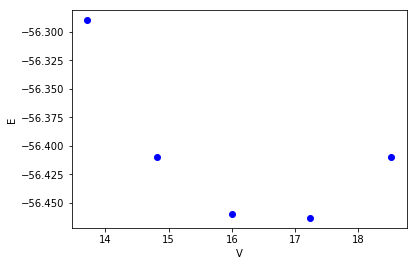
\includegraphics[width=.9\linewidth]{obipy-resources/513154bd4a2746455cb8d249e9b62785-85168upj.png}
\end{center}

In Materials Science we often want to fit an equation of state to this data. We will use this equation:

\(E = E_0 + \frac{B_0 V}{B_0'}\left(\frac{(V_0 / V)^{B_0'}}{B_0' - 1} + 1 \right) - \frac{V_0 B_0}{B_0' - 1}\)

from \url{https://journals.aps.org/prb/pdf/10.1103/PhysRevB.28.5480}. In this model there are four parameters:

\begin{center}
\begin{tabular}{ll}
name & desc\\
\hline
E\_0 & energy at the minimim\\
B\_0 & bulk modulus\\
B\_0' & first derivative of the bulk modulus\\
V\_0 & volume at the energy minimum\\
\end{tabular}
\end{center}

We would like to find the value of these parameters that best fits the data above. That means, find the set of parameters that minimize the sum of the errors between the model and data.

First we need a function that will use the parameters and return the energy for a given volume.

\begin{minted}[frame=lines,fontsize=\scriptsize,linenos]{ipython}
def Murnaghan(parameters, vol):
    'From PRB 28,5480 (1983)'
    E0, B0, BP, V0 = parameters
    E = E0 + B0 * vol / BP * \
        (((V0 / vol)**BP) / (BP - 1) + 1) - V0 * B0 / (BP - 1.)

    return E
\end{minted}

Next, we need a function that computes the summed squared errors for a set of parameters.

\begin{minted}[frame=lines,fontsize=\scriptsize,linenos]{ipython}
def objective(pars):
    err = energies - Murnaghan(pars, volumes)
    return np.sum(err**2)  # we return the summed squared error directly
\end{minted}

Finally,  we need an initial guess to start the minimization. As with all minimization problems, this can be the most difficult step. It is always a good idea to use properties of the model and data where possible to make these guesses. We have no way to plot anything in four dimensions, so we use analysis instead.

We can derive some of these from the data we have. First, we can get the minimum in energy and the corresponding volume that we know from the data. These are not the final answer, but they are a good guess for it.

The B\(_{\text{0}}\) parameter is related to the curvature at the minimum, which is the second derivative. We get that from repeated calls to \texttt{numpy.gradient}. Finally, \(B_0'\) is related to the derivative of \(B\) at the minimum, so we estimate that too.

\begin{minted}[frame=lines,fontsize=\scriptsize,linenos]{ipython}
imin = np.argmin(energies)
dedv = np.gradient(energies, volumes)
B = np.gradient(dedv, volumes)
Bp = np.gradient(B, volumes)


x0 = [energies[imin],
      B[imin],
      Bp[imin],
      volumes[imin]]
\end{minted}

Finally, we are ready to fit our function. As usual, we also plot the data and the fit for visual inspection.

\begin{minted}[frame=lines,fontsize=\scriptsize,linenos]{ipython}
from scipy.optimize import minimize
sol = minimize(objective, x0)
print(sol)

plt.plot(volumes, energies, 'bo', label='Data')
vfit = np.linspace(min(volumes), max(volumes))
plt.plot(vfit, Murnaghan(sol.x, vfit), label='fit')
plt.legend()
plt.xlabel('V')
plt.ylabel('E')
\end{minted}

\begin{verbatim}
     fun: 1.4912965344598558e-05
hess_inv: array([[  3.03863745e-01,  -3.02573371e+00,   8.04371522e+01,
        -2.41676767e+00],
      [ -3.02573371e+00,   5.27761683e+01,  -1.63584644e+03,
         4.76079594e+01],
      [  8.04371522e+01,  -1.63584644e+03,   7.06615880e+04,
        -2.81868629e+03],
      [ -2.41676767e+00,   4.76079594e+01,  -2.81868629e+03,
         1.54690538e+02]])
     jac: array([  3.46717718e-06,   1.36594349e-06,   7.79607490e-09,
       -5.30043053e-07])
 message: 'Optimization terminated successfully.'
    nfev: 216
     nit: 31
    njev: 36
  status: 0
 success: True
       x: array([-56.46839794,   0.57236216,   2.74084063,  16.55900277])

\end{verbatim}




\begin{center}
\includegraphics[width=.9\linewidth]{obipy-resources/513154bd4a2746455cb8d249e9b62785-85168WQx.png}
\end{center}

That looks pretty good. We should ask ourselves, how do we know we got a minimum? We should see that the objective function is really at a minimum \emph{for each of the parameters}. Here, we show that it is a minimum for the first parameter.

\begin{minted}[frame=lines,fontsize=\scriptsize,linenos]{ipython}
E0_range = np.linspace(0.9 * sol.x[0], 1.1 * sol.x[0])

errs = [objective([e0, *sol.x[1:]]) for e0 in E0_range]

plt.plot(E0_range, errs)
plt.axvline(sol.x[0], c='k', ls='--')
plt.xlabel('E0')
plt.ylabel('summed squared error')
\end{minted}

\begin{center}
\includegraphics[width=.9\linewidth]{obipy-resources/513154bd4a2746455cb8d249e9b62785-85168u3L.png}
\end{center}

You can see visually that the error goes up on each side of the parameter estimate.

\textbf{exercise} Repeat this analysis for the other three parameters.

Usually we do some regression to find one of these:
\begin{enumerate}
\item Parameters for the model - because the parameters mean something
\item Properties of the model - because the properties mean something
\end{enumerate}

In this particular case, we can do both. Some of the parameters are directly meaningful, like the E0, and V0 are the energy at the minimum, and the corresponding volume. B0 is also meaningful, it is called the bulk modulus, and it is a material property.

Now that we have a model though we can also define properties of it, e.g. \emph{in this case} we have from thermodynamics that \(P = -dE/dV\). We can use our model to define this derivative. I use \texttt{scipy.misc.derivative} for this for convenience. The only issue with it is the energy function has arguments that are not in the right order for the derivative, so I make a proxy function here that just reverses the order of the arguments.

\begin{minted}[frame=lines,fontsize=\scriptsize,linenos]{ipython}
from scipy.misc import derivative

pars = sol.x
def P(V):
    def proxy(V, pars):
        return Murnaghan(pars, V)
    dEdV = derivative(proxy, V, args=(pars,), dx=1e-6)
    return -dEdV

# Some examples
P(16), P(pars[-1]), P(18)
\end{minted}

\begin{verbatim}
(0.020610354312111667, -0.0, -0.042691265633720832)
\end{verbatim}

The result above shows that it takes positive pressure to compress the material, the pressure is zero at the minimum, and it takes negative pressure to cause it to expand.

This example is just meant to illustrate what one can do with a model once you have it.

\subsection{Parameter confidence intervals}
\label{sec:org229c15d}

We have left out an important topic in the discussion above: How certain are we of the parameters we estimated? This is a complicated question that requires moderately sophisticated statistics to answer. We will build up to the solution in steps.

First, we recall that in a statistical sense we are \emph{estimating} the values of the parameters. Specifically, we estimate the \emph{mean} of the parameters, from a fixed number of data points.

Let's say we have made 10 measurements that have an average of 16.1, and a standard deviation of 0.01. What is the range of values that we are 95\% confident the next measurement will fall in?

We have to take into account the fact that we only have 10 measurements to make the estimation from, so the estimate is more uncertain than if we have 100 or 1000 measurements. The student t-tables tell us precisely how much more uncertain depending on the confidence level you want.

The point here is not for you to memorize or derive these formulas, only to illustrate that the uncertainty is not simply the standard deviation. It also includes the effect of the sample size.

\begin{minted}[frame=lines,fontsize=\scriptsize,linenos]{ipython}
from scipy.stats.distributions import t

n = 10  # number of measurements
dof = n - 1  # degrees of freedom
avg_x = 16.1  # average measurement
std_x = 0.01  # standard deviation of measurements

# Find 95% prediction interval for next measurement
alpha = 1.0 - 0.95

pred_interval = t.ppf(1 - alpha / 2.0, dof) * std_x / np.sqrt(n)

plus_side = avg_x + pred_interval
minus_side = avg_x - pred_interval

print(f'We are 95% confident the next measurement will be between {minus_side:1.3f} and {plus_side:1.3f}')
\end{minted}

\begin{verbatim}
We are 95% confident the next measurement will be between 16.093 and 16.107

\end{verbatim}

To consider the uncertainty in model parameters, we need some way to estimate the standard deviation of the parameters. \texttt{scipy.optimize.minimize} does not provide much help with that. We will instead turn to \texttt{scipy.optimize.curve\_fit}.

\begin{minted}[frame=lines,fontsize=\scriptsize,linenos]{ipython}
import numpy as np
from scipy.optimize import curve_fit

curve_fit?
\end{minted}

\subsubsection{An example with curve\_fit}
\label{sec:org786168c}

Given the data below, fit the following curve:

\(y(x) = \frac{a x}{b + x}\) to it.

That means, estimate the values of \(a, b\) that best fit the data.

\begin{minted}[frame=lines,fontsize=\scriptsize,linenos]{ipython}
%matplotlib inline
import matplotlib.pyplot as plt

x = np.array([0.5, 0.387, 0.24, 0.136, 0.04, 0.011])
y = np.array([1.255, 1.25, 1.189, 1.124, 0.783, 0.402])

plt.plot(x, y, 'bo')
plt.xlabel('x')
plt.ylabel('y')
\end{minted}

\begin{center}
\includegraphics[width=.9\linewidth]{obipy-resources/513154bd4a2746455cb8d249e9b62785-92704lhH.png}
\end{center}

What should we use for an initial guess? At \(x=0\), \(y = 0\), which isn't that helpful. At large \(x\), we have \(y=a\). From the data, we can guess that \(a \approx 1.2\). For small x, we have \(y = a/b x\). So, if we estimate the slope, we can estimate b.

\begin{minted}[frame=lines,fontsize=\scriptsize,linenos]{ipython}
a0 = 1.2
m = np.gradient(y, x, edge_order=2) # m = a / b  ->  b = a / m

b0 = a0 / m[-1]
a0, b0
\end{minted}

\begin{verbatim}
(1.2, 0.078115603236335401)
\end{verbatim}

Now for the fitting.

\begin{minted}[frame=lines,fontsize=\scriptsize,linenos]{ipython}
# this is the function we want to fit to our data
def func(x, a, b):
    return a * x / (b + x)

initial_guess = [a0, b0]
pars, pcov = curve_fit(func, x, y, p0=initial_guess)

pars, pcov
\end{minted}

\begin{verbatim}
(array([ 1.32753143,  0.02646156]),
 array([[  9.45332917e-05,   7.10675655e-06],
        [  7.10675655e-06,   1.05658850e-06]]))
\end{verbatim}

\emph{Always} check the fit visually.

\begin{minted}[frame=lines,fontsize=\scriptsize,linenos]{ipython}
plt.plot(x, y, 'bo')
xfit = np.linspace(0, 0.5)
plt.plot(xfit, func(xfit, *pars))
plt.xlabel('x')
plt.ylabel('y')
plt.legend(['data', 'fit'])
\end{minted}

\begin{center}
\includegraphics[width=.9\linewidth]{obipy-resources/513154bd4a2746455cb8d249e9b62785-92704yrN.png}
\end{center}

\textbf{exercise} Try different initial guesses and find one that does not look this good.

\subsubsection{Uncertainty estimation}
\label{sec:org3549911}

Recall from the documentation of curve\_fit that the standard deviation of each parameter is defined by:

\begin{minted}[frame=lines,fontsize=\scriptsize,linenos]{ipython}
np.sqrt(np.diag(pcov))
\end{minted}

\begin{verbatim}
array([ 0.00972282,  0.0010279 ])
\end{verbatim}

We can use these to estimate confidence intervals on the two parameters.

\begin{minted}[frame=lines,fontsize=\scriptsize,linenos]{ipython}
from scipy.stats.distributions import t

alpha = 0.05  # 95% confidence interval = 100*(1-alpha)

n = len(y)    # number of data points
p = len(pars)  # number of parameters

dof = max(0, n - p)  # number of degrees of freedom

# student-t value for the dof and confidence level
tval = t.ppf(1.0 - alpha / 2., dof)

for i, p, var in zip(range(n), pars, np.diag(pcov)):
    sigma = var**0.5
    print(f'p{i}: {p:1.2f} [{p - sigma * tval:1.3f}  {p + sigma * tval:1.3f}]')
\end{minted}

\begin{verbatim}
p0: 1.33 [1.301  1.355]
p1: 0.03 [0.024  0.029]

\end{verbatim}

The interpretation of this is that we do not know exactly what the parameters are, but we can be 95\% confident that they fall in these ranges. These ranges do not include zero, so that is an indication that the parameters are significant.

It is \emph{not expected} that you learn all the details above. They have been coded into the "Python computations in science and engineering" \href{https://kitchingroup.cheme.cmu.edu/pycse/}{pycse} package. This is not part of Anaconda; you have to install it yourself. This code block should do that and install some dependencies (you only need to run it once).

\begin{minted}[frame=lines,fontsize=\scriptsize,linenos]{ipython}
!pip install uncertainties
!pip install quantities
!pip install pycse
\end{minted}



After that, you can import the nlinfit command and use it to get confidence intervals directly.

\begin{minted}[frame=lines,fontsize=\scriptsize,linenos]{ipython}
from pycse import nlinfit

nlinfit?
\end{minted}

\begin{minted}[frame=lines,fontsize=\scriptsize,linenos]{ipython}
pars, pars_ci, se = nlinfit(func, x, y, [a0, b0])

for i, par in enumerate(pars):
    print(f'{par:1.3f}, {np.round(pars_ci[i], 3)}, {se[i]:1.4f}')
\end{minted}

\begin{verbatim}
1.328, [ 1.301  1.355], 0.0097
0.026, [ 0.024  0.029], 0.0010

\end{verbatim}

It is important to realize that:
\begin{enumerate}
\item The size of the confidence interval depends on the number of parameters, data points, and desired confidence level.
\item The root of this is the minimization of an error function.
\end{enumerate}

\subsubsection{What about uncertainty on the predictions?}
\label{sec:org7bdbeb6}

Consider the fit again, and extrapolate it to larger \(x\):

\begin{minted}[frame=lines,fontsize=\scriptsize,linenos]{ipython}
plt.plot(x, y, 'bo')
xfit = np.linspace(0, 5)
plt.plot(xfit, func(xfit, *pars))
plt.xlabel('x')
plt.ylabel('y')
plt.legend(['data', 'fit'])
func(xfit, *pars)[-1]
\end{minted}

\begin{verbatim}
1.3205427044923441
\end{verbatim}



\begin{center}
\includegraphics[width=.9\linewidth]{obipy-resources/513154bd4a2746455cb8d249e9b62785-92704zes.png}
\end{center}


We estimate the model plateaus at about y=1.32, but what is an appropriate estimate of the error in this? There are uncertainties in the model parameters, so there must be uncertainty in the predictions. To estimate this, we first look at how to generate a distribution of random numbers with a normal distribution around some mean with some standard error.

\begin{minted}[frame=lines,fontsize=\scriptsize,linenos]{ipython}
p0_mean = pars[0]
p0_se = se[0]

p0_dist = np.random.normal(p0_mean, p0_se, 5000)
plt.hist(p0_dist, bins=20)
\end{minted}

\begin{verbatim}
(array([   5.,   11.,   34.,   76.,  146.,  284.,  482.,  616.,  759.,
         739.,  633.,  489.,  358.,  221.,   87.,   40.,   15.,    4.,
           0.,    1.]),
 array([ 1.29380418,  1.29747208,  1.30113998,  1.30480788,  1.30847578,
         1.31214368,  1.31581159,  1.31947949,  1.32314739,  1.32681529,
         1.33048319,  1.33415109,  1.33781899,  1.34148689,  1.34515479,
         1.34882269,  1.35249059,  1.35615849,  1.35982639,  1.36349429,
         1.36716219]),
 <a list of 20 Patch objects>)
\end{verbatim}



\begin{center}
\includegraphics[width=.9\linewidth]{obipy-resources/513154bd4a2746455cb8d249e9b62785-92704zlg.png}
\end{center}

So the idea is we can generate a distribution of the parameters

\begin{minted}[frame=lines,fontsize=\scriptsize,linenos]{ipython}
p1_dist = np.random.normal(pars[1], se[1], 5000)

y5 = [func(5, p0, p1) for p0, p1 in zip(p0_dist, p1_dist)]
plt.hist(y5)

np.mean(y5), np.std(y5)
\end{minted}

\begin{verbatim}
(1.3204084851395486, 0.0095732578745979444)
\end{verbatim}



\begin{center}
\includegraphics[width=.9\linewidth]{obipy-resources/513154bd4a2746455cb8d249e9b62785-92704N6s.png}
\end{center}

Well, in 20/20 hindsight, we might have guessed the uncertainty in the asymptote would be just like the uncertainty in the \(a\) parameter. In this case, it is appropriate to use three significant figures given the uncertainty on the answer. A useful guideline is that the 95\% confidence interval is about \textpm{} 2 \(\sigma\). At \textpm{} 1 \(\sigma\) you only have about a 60\% confidence interval.

\begin{minted}[frame=lines,fontsize=\scriptsize,linenos]{ipython}
print(f'At x=5, y={np.mean(y5):1.3f} +- {2 * np.std(y5):1.3f} at about the 95% confidence level.')
\end{minted}

\begin{verbatim}
At x=5, y=1.320 +- 0.019 at about the 95% confidence level.

\end{verbatim}

So we are not that uncertain after all in this case.

This method of error propagation is not perfect as it assumes the errors between the parameters are independent, and that they are normally distributed. However, the method is very simple to do, and simply relies on sampling the parameters from their respective distributions, and letting the results propagate naturally through the model. You do need to check for convergence with the sample size. This method is called a Monte Carlo propagation of errors.

\textbf{Exercise} An alternative approach to uncertainty propagation is the \href{https://pythonhosted.org/uncertainties/index.html}{uncertainties} package. This should have been installed with pycse above. Here is an example of using it. The gist is you define special objects that know their uncertainty, and allow the package to handle the uncertainties for you.


\begin{minted}[frame=lines,fontsize=\scriptsize,linenos]{ipython}
from uncertainties import ufloat

a = ufloat(pars[0], se[0])
b = ufloat(pars[1], se[1])

x = 5

print(a * x / (b + x))
\end{minted}

\begin{verbatim}
1.321+/-0.010

\end{verbatim}

Note that it outputs \textpm{} a standard deviation. You \emph{always} have to know what the \textpm{} means, and it doesn't say you assume it is \textpm{} 1 \(\sigma\). The result above is similar to the Monte Carlo results. You should check those for convergence!

There are some caveats with the \texttt{uncertainties} package.
\begin{enumerate}
\item It is great for simple algebra.
\item It does not work for all functions, e.g. through fsolve, or solve\_ivp, without doing some extra work on your part.
\end{enumerate}

\subsection{Summary}
\label{sec:org0a7a298}

We covered a lot of ground today. The key points are:
\begin{enumerate}
\item Regression is a minimization of an accumulated error function.
\item If you need uncertainty on the parameters from a regression, use \texttt{pycse.nlinfit}.
\item If you need uncertainty on model predictions, you can either simulate it, or use a package like \texttt{uncertainties} to estimate it.
\end{enumerate}

\section{12 Lies, damn lies, and statistics}
\label{sec:org521d8a1}

\subsection{Uncertainty estimates from curvefit and scipy.optimize.minimize}
\label{sec:orge81586f}

We previously examined how to estimate uncertainty from the covariance matrix returned from curve\_fit. Recall we need the diagonal of the covariance matrix, which is estimated during the fitting. We will consider fitting a line to the following data.

\begin{minted}[frame=lines,fontsize=\scriptsize,linenos]{ipython}
import numpy as np
from scipy.optimize import curve_fit

x = np.array([0.,    2.5,   5.,    7.5,  10. ])
y = np.array([1.14,    1.91,  2.48,  2.2,  4.0])

def model(x, m, b):
    return m * x + b

p, pcov = curve_fit(model, x, y, [0.2, 0.1])
print(p)
pcov
\end{minted}

\begin{verbatim}
[ 0.2404      1.14399999]

\end{verbatim}

\begin{verbatim}
array([[ 0.00430672, -0.0215336 ],
       [-0.0215336 ,  0.161502  ]])
\end{verbatim}

\texttt{scipy.optimize.minimize} does not return the covariance matrix; with \emph{some} of the methods, it returns an estimate of the inverse Hessian matrix. In theory, the covariance matrix and the inverse hessian are related to each other with \(cov = 0.5 * H^{-1}\).

\begin{minted}[frame=lines,fontsize=\scriptsize,linenos]{ipython}
from scipy.optimize import minimize

def model(pars, x):
    x = np.array(x)
    m, b = pars
    return m * x + b

def objective(pars):
    errs = y - model(pars, x)
    return np.sum(errs**2)

sol = minimize(objective, [0.2, 1])
print(sol.x)
0.5 * sol.hess_inv
\end{minted}

\begin{verbatim}
[ 0.2404      1.14399997]

\end{verbatim}

\begin{verbatim}
array([[ 0.01019113, -0.06596866],
       [-0.06596866,  0.49131361]])
\end{verbatim}

That doesn't look very good. \textbf{But}, remember that it is an estimate of the Hessian and we need to be careful about the accuracy. The minimizer terminates when the solution reaches the tolerance, \emph{not} when the Hessian is accurate!

\begin{minted}[frame=lines,fontsize=\scriptsize,linenos]{ipython}
sol = minimize(objective, [0.2, 1], tol=1e-9)
print(sol.x)
print(0.5 * sol.hess_inv)
\end{minted}

\begin{verbatim}
[ 0.24039999  1.144     ]
[[ 0.00424425 -0.02201408]
 [-0.02201408  0.16613705]]

\end{verbatim}

With the increased accuracy, you can see the covariance is approximately equal to 1/2 the inverse Hessian. That means you can use it to estimate the uncertainty in the same way we did with curve\_fit.

Not all solvers generate the inverse Hessian matrix, e.g. \texttt{SLSQP} does not do it. You have three options. One is always to compute the Hessian analytically. The other two options rely on libraries that use automatic differentiation to compute the relevant derivatives. One is to use numdifftools (which you may have to install). Either way, you have to compute the Hessian on the objective function that is being minimized

\begin{minted}[frame=lines,fontsize=\scriptsize,linenos]{ipython}
import numdifftools as nd

def f(pars):
    m, b = pars
    return np.sum((y - (m * x + b))**2)

H = nd.Hessian(f)
0.5 * np.linalg.inv(H(p))
\end{minted}

\begin{verbatim}
array([[ 0.004, -0.02 ],
       [-0.02 ,  0.15 ]])
\end{verbatim}


The final option is to use \texttt{autograd} (which you may also have to install).

\begin{minted}[frame=lines,fontsize=\scriptsize,linenos]{ipython}
import autograd.numpy as np
from autograd import hessian

h = hessian(f)
0.5 * np.linalg.inv(h(p))
\end{minted}

\begin{verbatim}
array([[ 0.004, -0.02 ],
       [-0.02 ,  0.15 ]])
\end{verbatim}

Now you can use these to estimate the uncertainties even for optimizers that don't provide the estimated inverse Hessian.

\subsection{Effects of outliers on regression}
\label{sec:orgc8ee8da}

Outliers can have a significant effect on the fit of a model to data. Let's consider this example, where we want to fit a line to some data that has an outlier in it. This is just a linear regression, and we start out using \texttt{numpy.polyfit}.

\begin{minted}[frame=lines,fontsize=\scriptsize,linenos]{ipython}
import numpy as np
%matplotlib inline
import matplotlib.pyplot as plt

x = [0.,    2.5,   5.,    7.5,  10. ]
y = [1.14,    1.91,  2.48,  2.2,  4.0]

p = np.polyfit(x, y, 1)
print(p)
xfit = np.linspace(0, 10)

plt.plot(x, y, 'bo')
plt.plot(xfit, np.polyval(p, xfit));
plt.xlabel('x')
plt.ylabel('y')
\end{minted}

\begin{verbatim}
[ 0.2404  1.144 ]

\end{verbatim}




\begin{center}
\includegraphics[width=.9\linewidth]{obipy-resources/37c51028cef42d76546d882661b04271-4039131w.png}
\end{center}

You can see that the fitted line is "dragged" towards the outlier. We say that least squares minimization is not \emph{robust} to outliers.

This may be undesirable because if you believe there is an outlier, perhaps due to experimental error, then this point affects the accuracy of the model more than the other points you believe to be more accurate.

Today we will consider a variety of approaches to minimize the effects of outliers. We first begin by re-examining how these parameters are obtained. Here, we illustrate that the results from polyfit are equivalent to minimizing the summed squared errors between the model and the data.

\begin{minted}[frame=lines,fontsize=\scriptsize,linenos]{ipython}
from scipy.optimize import minimize

def model(pars, x):
    x = np.array(x)
    m, b = pars
    return m * x + b

def objective(pars):
    errs = y - model(pars, x)
    return np.sum(errs**2)

minimize(objective, [0.2, 1])
\end{minted}

\begin{verbatim}
     fun: 0.8075100000000078
hess_inv: array([[ 0.02038226, -0.13193732],
      [-0.13193732,  0.98262721]])
     jac: array([  5.28991222e-07,  -3.05473804e-07])
 message: 'Optimization terminated successfully.'
    nfev: 20
     nit: 2
    njev: 5
  status: 0
 success: True
       x: array([ 0.2404    ,  1.14399997])
\end{verbatim}

The problem is that we are minimizing the error\(^{\text{2}}\), which puts more weight on large errors than small errors.

Least squares regression is also called L\(_{\text{2}}\) norm regression

\subsubsection{Minimizing the summed absolute errors}
\label{sec:org6c4e45e}

We can choose to minimize another objective function, for example the summed absolute value of the errors. This will reduce the emphasis on large errors. This is  also called L\(_{\text{1}}\) norm regression.

\begin{minted}[frame=lines,fontsize=\scriptsize,linenos]{ipython}
def objective(pars):
    errs = y - model(pars, x)
    return np.sum(np.abs(errs))

L1_sol = minimize(objective, [0.2, 1])
print(L1_sol.x)
plt.plot(x, y, 'bo')
plt.plot(xfit, model(L1_sol.x, xfit))
\end{minted}

\begin{verbatim}
[ 0.26845682  1.14      ]

\end{verbatim}

\begin{verbatim}
[<matplotlib.lines.Line2D at 0x117bf3b70>]
\end{verbatim}



\begin{center}
\includegraphics[width=.9\linewidth]{obipy-resources/37c51028cef42d76546d882661b04271-20264wuA.png}
\end{center}

There is a historical reason this is not done a lot, and that is the absolute value function has a discontinuity in its first derivative which can be problematic in some optimization algorithms. It is obviously not a problem here, and you can see that the outlier has less of an effect on the fitted line in this case.

Finally, we can generalize these ideas to something called L\(_{\text{p}}\) norm regressions where we seek to minimize:

\(\sum |\epsilon_i|^p\)

In \href{https://www.tandfonline.com/doi/abs/10.1080/00401706.1972.10488892}{this paper} a value of \(p=1.5\) is recommended for general use. Note this is less than two, and greater than one, so it is expected to have an intermediate effect compared to L\(_{\text{1}}\) and L\(_{\text{2}}\) norm regression.

\begin{minted}[frame=lines,fontsize=\scriptsize,linenos]{ipython}
def objective(pars):
    p = 1.5
    errs = y - model(pars, x)
    return np.sum(np.abs(errs)**p)

Lp_sol = minimize(objective, [0.2, 1])
print(Lp_sol.x)
plt.plot(x, y, 'bo')
plt.plot(xfit, model(Lp_sol.x, xfit))
\end{minted}

\begin{verbatim}
[ 0.25741034  1.15352086]

\end{verbatim}

\begin{verbatim}
[<matplotlib.lines.Line2D at 0x11ab9b630>]
\end{verbatim}



\begin{center}
\includegraphics[width=.9\linewidth]{obipy-resources/37c51028cef42d76546d882661b04271-20264ZIt.png}
\end{center}


\subsubsection{Robust regression approaches}
\label{sec:org3db24d4}

An alternative approach to least squares or absolute error minimization is called robust regression (see Applied Regression Analysis, 3rd edition, Draper and Smith, chapter 25). This is a class of methods that uses a different metric to minimize in the objective function.

The simplest approach is to minimize the median of the squared error. Recall that minimizing the sum of squared errors is practically like minimizing the average squared error. If you have a symmetric distribution of errors, then the mean and median are practically the same. If there is an outlier, however, the mean will be skewed towards the outlier, while the median will be at a position that splits the distribution in half, and is closer to what you believe the mean to be.

Here we show that given an asymmetric distribution, the median is smaller than the mean.

\begin{minted}[frame=lines,fontsize=\scriptsize,linenos]{ipython}
errs = np.array([0.1, 0.01, 0.05, 0.02, 0.8])
s = errs**2
plt.hist(s, normed=True)
plt.axvline(np.mean(s), color='r')
plt.axvline(np.median(s), color='k')
plt.legend(['mean', 'median'])
plt.xlabel('')
\end{minted}

\begin{center}
\includegraphics[width=.9\linewidth]{obipy-resources/37c51028cef42d76546d882661b04271-20264ypa.png}
\end{center}

\begin{enumerate}
\item Least Median regression
\label{sec:org184f2b4}

It is straightforward to modify the objective function to minimize the median of the squared errors.

\begin{minted}[frame=lines,fontsize=\scriptsize,linenos]{ipython}
def objective(pars):
    errs = y - model(pars, x)
    return np.median(errs**2)

LMS_sol = minimize(objective, [0.2, 1])
print(LMS_sol.x)
plt.plot(x, y, 'bo')
plt.plot(xfit, model(LMS_sol.x, xfit))
\end{minted}

\begin{verbatim}
[ 0.26804924  1.18981534]

\end{verbatim}

\begin{verbatim}
[<matplotlib.lines.Line2D at 0x116d345f8>]
\end{verbatim}



\begin{center}
\includegraphics[width=.9\linewidth]{obipy-resources/37c51028cef42d76546d882661b04271-20264XNT.png}
\end{center}
\end{enumerate}

\subsubsection{Weighted nonlinear regression}
\label{sec:orgfbf5cff}

Outliers often are associated with larger uncertainties about their values. An alternative approach to the methods described above is to use weights to say how important each data point is. This example is adapted from \url{https://www.mathworks.com/help/stats/examples/weighted-nonlinear-regression.html}

\begin{minted}[frame=lines,fontsize=\scriptsize,linenos]{ipython}
import numpy as np
%matplotlib inline
import matplotlib.pyplot as plt

x = [1, 2, 3, 5, 7, 10]
y = [109, 149, 149, 191, 213, 224]
plt.plot(x, y, 'bo')
plt.xlabel('Incubation (days)')
plt.ylabel('BOD')
\end{minted}

\begin{center}
\includegraphics[width=.9\linewidth]{obipy-resources/37c51028cef42d76546d882661b04271-20264NNW.png}
\end{center}

The aim of this work is to fit a nonlinear model \(y= a (1 - e^{-b x})\) to this data. We first consider a standard minimization of the sum squared errors.

\begin{minted}[frame=lines,fontsize=\scriptsize,linenos]{ipython}
def model(pars, x):
    a, b = pars
    x = np.array(x)
    return a * (1 - np.exp(-b * x))

def objective(pars):
    errs = y - model(pars, x)
    return np.sum(errs**2)


guesses = [240, 0.5]

from scipy.optimize import minimize

sol = minimize(objective, guesses)
pars = sol.x

plt.plot(x, y, 'bo')
xfit = np.linspace(0, 10)
plt.plot(xfit, model(pars, xfit))
plt.xlabel('Incubation (days)')
plt.ylabel('BOD')
\end{minted}

\begin{center}
\includegraphics[width=.9\linewidth]{obipy-resources/37c51028cef42d76546d882661b04271-20264aXc.png}
\end{center}

The fit generally goes through the data, but it is not clear if there is a small outlier near 2 that is skewing the fit, and perhaps leading to an inaccurate asymptote at long times.

Suppose, however, that these data points represent averages from multiple measurements, and we only measured the first two point once, and the rest of the points 5 times. In this case, we might want to put more \emph{weight} on the points we measured multiple times.

We achieve this by modifying the objective function, in this case multiplying each error by the number of times the measurement was made. This makes reducing errors on points we measured a lot more important than the points we measured less.

\begin{minted}[frame=lines,fontsize=\scriptsize,linenos]{ipython}
w = np.array([1, 1, 5, 5, 5, 5])

def objective(pars):
    errs = (y - model(pars, x)) * w
    return np.sum(errs**2)


guesses = [240, 0.5]

from scipy.optimize import minimize

sol = minimize(objective, guesses)
pars = sol.x
print(pars)
plt.plot(x, y, 'bo')
xfit = np.linspace(0, 10)
plt.plot(xfit, model(pars, xfit))
plt.xlabel('Incubation (days)')
plt.ylabel('BOD')
\end{minted}

\begin{verbatim}
[ 230.77020941    0.35563065]

\end{verbatim}




\begin{center}
\includegraphics[width=.9\linewidth]{obipy-resources/37c51028cef42d76546d882661b04271-20264nhi.png}
\end{center}

The result here is that the model fits the points we measured a lot better than the points we measured once.



There are many ways you could choose to weight the points depending on what you know about them. If you have uncertainties about the measured data, you can weight the points accordingly, e.g. defining the weights as inversely proportional to the uncertainty.
\subsection{Regression with constrained parameters}
\label{sec:orgde348f1}

Consider this data, which we wish to fit a line to, and suppose we know that the intercept has some physical meaning, e.g. an initial concentration. In this case, it is an error to have a negative value for the intercept.

\begin{minted}[frame=lines,fontsize=\scriptsize,linenos]{ipython}
x = np.array([ 0.        ,  0.55555556,  1.11111111,  1.66666667,  2.22222222,
               2.77777778,  3.33333333,  3.88888889,  4.44444444,  5.        ])
y = np.array([-0.50545117,  0.77599028,  2.64586101,  3.12921576,  5.1337751 ,
              5.10184953,  6.35692171,  8.55711734,  9.79718111,  9.3069269 ])

plt.plot(x, y, 'bo')
np.polyfit(x, y, 1)
\end{minted}

\begin{verbatim}
array([ 2.08000595, -0.17007613])
\end{verbatim}



\begin{center}
\includegraphics[width=.9\linewidth]{obipy-resources/37c51028cef42d76546d882661b04271-2026405Q.png}
\end{center}

What we want in this case is to \emph{constrain} the regression model to penalize negative values for the intercept. A simple way to do this to simply add the absolute value of the intercept (or something proportional to it) to the objective function. The proportionality determines the importance of the penalty, and you may have to adjust it to get the performance you want. The absolute value is sometimes problematic for the default solver in minimize.

\begin{minted}[frame=lines,fontsize=\scriptsize,linenos]{ipython}
def model(pars, x):
    m, b = pars
    return m * x + b

def objective(pars):
    m, b = pars
    errs = y - model(pars, x)
    a = 1
    return np.sum(errs**2) + a * np.abs(b)

minimize(objective, [2, 0])
\end{minted}

\begin{verbatim}
     fun: 3.1903861026378357
hess_inv: array([[  6.84348734e-03,   7.56073454e-06],
      [  7.56073454e-06,   6.80554654e-08]])
     jac: array([ -1.09505653e-03,   1.90831292e+00])
 message: 'Desired error not necessarily achieved due to precision loss.'
    nfev: 676
     nit: 11
    njev: 166
  status: 2
 success: False
       x: array([  2.03166230e+00,  -5.66444458e-10])
\end{verbatim}

The problem arises from the discontinuity in the derivative of the at the point we need it for the absolute value function. One solution is to use a solver that is more robust than BFGS, like the Nelder-Mead solver.

\begin{minted}[frame=lines,fontsize=\scriptsize,linenos]{ipython}
con_sol = minimize(objective, [2, 0.0], method='Nelder-Mead')
print(con_sol)
\end{minted}

\begin{verbatim}
final_simplex: (array([[  2.03168335e+00,  -2.69088745e-05],
      [  2.03172913e+00,  -7.13996887e-05],
      [  2.03163452e+00,  -1.12785339e-04]]), array([ 3.19038652,  3.19038735,  3.19038825]))
          fun: 3.1903865188524301
      message: 'Optimization terminated successfully.'
         nfev: 36
          nit: 19
       status: 0
      success: True
            x: array([  2.03168335e+00,  -2.69088745e-05])

\end{verbatim}

Alternatively, you can use a penalty function that is continuous in derivatives at x=0 like this. Note that here you have to adjust the proportionality constant to be large since b\(^{\text{2}}\) goes to zero at zero quickly.

\begin{minted}[frame=lines,fontsize=\scriptsize,linenos]{ipython}
def objective(pars):
    m, b = pars
    errs = y - model(pars, x)
    a = 100
    return np.sum(errs**2) + a * b**2

minimize(objective, [2, 0])
\end{minted}

\begin{verbatim}
     fun: 3.188030443914453
hess_inv: array([[ 0.15851995, -0.37666981],
      [-0.37666981,  0.92875501]])
     jac: array([  1.19209290e-07,   3.87430191e-07])
 message: 'Optimization terminated successfully.'
    nfev: 20
     nit: 2
    njev: 5
  status: 0
 success: True
       x: array([ 2.0330284 , -0.00478475])
\end{verbatim}

This is an example of constrained minimization. There are many more approaches than described here. It is possible to minimize functions with a variety of equality and inequality constraints, as well as to specify bounds on the values of parameters.

\subsection{Summary}
\label{sec:orgc7f2d8e}

Regression is an important technical skill required in modern engineering. It is the method which we use to convert data into models.

At the core, regression involves minimization of some error function. The standard method is to minimize the summed squared error between the model and data. There are some benefits to this method: it is straight forward and there are well established methods to estimate the uncertainty in the parameters. However, it is known to be sensitive to outliers.

A variety of alternative approaches exist to reduce the influence of outliers, including minimizing the summed absolute errors, robust regression methods, and weighted regression methods. It is not always obvious what the right method to use is, this takes experience and an understanding of what you know about the model, the data, and the goals of the regression.

\section{13 review?}
\label{sec:org4ce755d}

\section{14 Constrained minimization}
\label{sec:org81fef08}

So far we have predominantly focused on unconstrained minimization. Sometimes, however, we seek to minimize an objective function and find solutions that meet some kind of constraint.

For example, in the last exam we wanted to find the minimum cost of a can that had a specific volume. The volume in this problem leads to an equality constraint, and we used the method of elimination to solve it. In other problems, we might simply require some part of the solution to be less than or greater than some number. We call these inequality constraints.

Here we will consider a strategy for solving these kinds of problems.

\subsection{scipy.optimize.minimize with constraints}
\label{sec:org8c1ef2d}

\texttt{scipy.optimize.minimize} can be used with constraints. Before we get to how this is done, we need to introduce a new data type in Python: the dictionary.

A dictionary, also known as a lookup or hash table, is a data structure that allows you to look up values by a key. A dictionary is created with curly brackets \{\} that contain \texttt{key: value} pairs. You can use anything that is "hashable" as a key, and anything as a value. Things that are hashable are: strings, numbers, tuples. You cannot use a list or array; they are mutable and not hashable. Here is an example.

\begin{minted}[frame=lines,fontsize=\scriptsize,linenos]{ipython}
def f(x):
    return x**2

d = {'a': 1,
     'type': 'function',
     'func': f,
     4: 'int',
     5.0: 'float'}
\end{minted}

Now, we can retrieve data from it like this:

\begin{minted}[frame=lines,fontsize=\scriptsize,linenos]{ipython}
d['a'], d[4], d[5.0]
\end{minted}

\begin{verbatim}
(1, 'int', 'float')
\end{verbatim}

It is usually an error to ask for a key that does not exist.

\begin{minted}[frame=lines,fontsize=\scriptsize,linenos]{ipython}
d['NotHere']
\end{minted}

\begin{verbatim}

KeyErrorTraceback (most recent call last)
<ipython-input-22-e786609d9548> in <module>()
----> 1 d['NotHere']

KeyError: 'NotHere'
\end{verbatim}


But, here is a little surprise:

\begin{minted}[frame=lines,fontsize=\scriptsize,linenos]{ipython}
d[5], d[5.0], hash(5), hash(5.0)
\end{minted}

\begin{verbatim}
('float', 'float', 5, 5)
\end{verbatim}

The integer 5 and float 5.0 hash to the same value, so the dictionary returns something for both of them.


We can get the function, and call it:

\begin{minted}[frame=lines,fontsize=\scriptsize,linenos]{ipython}
d['func'](3)
\end{minted}

\begin{verbatim}
9
\end{verbatim}

The reason we have to consider dictionaries is that \texttt{scipy.optimize.minimize} uses dictionaries to specify constraints.

\begin{minted}[frame=lines,fontsize=\scriptsize,linenos]{ipython}
from scipy.optimize import minimize
?minimize
\end{minted}

We have to write functions that codify the constraints, and then pass them to minimize.

\subsection{Equality constraints}
\label{sec:org677df4e}

The volume of a cylindrical can is \(V = (\pi/4) D^2 L\). The cost of the top/bottom of the can is $\backslash$$0.025 / cm\(^{\text{2}}\), and the cost of the sides is $\backslash$$0.043 / cm\(^{\text{2}}\). If we require a volume of 355 cm\(^{\text{3}}\), what is the optimal length and diameter to minimize the cost of the can?

We have two variables to modify: \(D, L\), but there is an equality constraint in this problem that is described in the volume equation. We codify this in a function that returns zero when the constraint is satisfied. We also define a variable for the constraints dictionary.

\begin{minted}[frame=lines,fontsize=\scriptsize,linenos]{ipython}
import numpy as np

def equality_constraint(x):
    D, L = x
    radius = D / 2
    V = np.pi * radius**2 * L
    return V - 355

constraints = {'type': 'eq', 'fun': equality_constraint}
\end{minted}

Now, we can setup the objective function with the two variables we want to vary to find the minimum.

\begin{minted}[frame=lines,fontsize=\scriptsize,linenos]{ipython}
cost_top = 0.025  # $/cm^2
cost_side = 0.043 # $/cm^2

def objective(x):
    D, L = x
    radius = D / 2
    top_area = np.pi * radius**2
    side_area = L * np.pi * D
    cost = (2 * top_area * cost_top) + (side_area * cost_side)
    return cost

sol = minimize(objective, (9.2, 5), constraints=constraints)
equality_constraint(sol.x)
objective(sol.x)
sol
\end{minted}

\begin{verbatim}
    fun: 9.960758701245243
    jac: array([ 1.44435978,  1.24215055])
message: 'Optimization terminated successfully.'
   nfev: 28
    nit: 7
   njev: 7
 status: 0
success: True
      x: array([ 9.19508759,  5.34597263])
\end{verbatim}


You can have multiple equality constraints, you just make a list of dictionaries. Suppose we seek to minimize \(x1 + x2 + x3^2\) subject to the equality constraints \(x1=1\), and \(x1^2 + x2^2 = 1\). Some analysis suggests that this really means x1=1, x2=0, and then x3 must also be zero to minimize the function, which has a minimum value of 1.


Here we can set this up as a minimization problem:

\begin{minted}[frame=lines,fontsize=\scriptsize,linenos]{ipython}
def objective(x):
    x1, x2, x3 = x
    return x1 + x2 + x3**2

def eq1(x):
    x1, x2, x3 = x
    return x1 - 1   # x = 1

def eq2(x):
    x1, x2, x3 = x
    return x1**2 + x2**2 - 1  # x1**2 + x2**2 = 1

constraints = [{'type': 'eq', 'fun': eq1},
               {'type': 'eq', 'fun': eq2}]

minimize(objective, [0, 0, 0], constraints=constraints)
\end{minted}

\begin{verbatim}
    fun: 1.0000051566408261
    jac: array([ 1.        ,  1.        , -0.00425012])
message: 'Optimization terminated successfully.'
   nfev: 409
    nit: 65
   njev: 65
 status: 0
success: True
      x: array([  1.00000000e+00,   6.40736032e-07,  -2.12506583e-03])
\end{verbatim}

\subsection{Inequality constraints}
\label{sec:org841acc1}

Inequality constraints are those where some part of the solution is greater than or less than a value. In \texttt{scipy.optimize.minimize} we codify this by writing functions that are non-negative, i.e. greater than or equal to zero at the solution.

Maximize \(x^3 - 3x\) subject to \(x \le 2\). First, recall we can rewrite the inequality as \(-x \ge -2\), and again as \(-x + 2 \ge 0\). That means for our solution we require \(-x+2\) to be positive. Also, since we are maximizing the function, our objective is multiplied by -1. When possible, it is always a good idea to visualize the problem:

\begin{minted}[frame=lines,fontsize=\scriptsize,linenos]{ipython}
def objective(x):
    return -1 * (x**3 - 3 * x)

%matplotlib inline
import matplotlib.pyplot as plt

x = np.linspace(-3, 3)
plt.plot(x, objective(x))
plt.axvline(2, color='k')
\end{minted}

\begin{center}
\includegraphics[width=.9\linewidth]{obipy-resources/e6e76468db53af7dc15a5007a7e59920-658373ja.png}
\end{center}

You can see by inspection there is a minimum around x=-1, and at x=2. Note the one at x=2 is not a minimum in the sense that the derivative=0 there, it is just the smallest value that also satisfies the constraint. To solve this problem, we set up the following code:

\begin{minted}[frame=lines,fontsize=\scriptsize,linenos]{ipython}
def ieq(x):
    return -x + 2

constraints = {'type': 'ineq', 'fun': ieq}

minimize(objective, 3, constraints=constraints)
\end{minted}

\begin{verbatim}
    fun: -1.99999999997004
    jac: array([-9.00000012])
message: 'Optimization terminated successfully.'
   nfev: 6
    nit: 2
   njev: 2
 status: 0
success: True
      x: array([ 2.])
\end{verbatim}

Note that there are two solutions. Which one you get depends on your initial guess.

\begin{minted}[frame=lines,fontsize=\scriptsize,linenos]{ipython}
minimize(objective, -0.9, constraints=constraints)
\end{minted}

\begin{verbatim}
    fun: -1.999999999942188
    jac: array([  2.63750553e-05])
message: 'Optimization terminated successfully.'
   nfev: 13
    nit: 4
   njev: 4
 status: 0
success: True
      x: array([-0.99999561])
\end{verbatim}

\subsection{An application}
\label{sec:orgc6ff88b}

Let us suppose that a merry farmer has 75 roods (4 roods = 1 acre) on which to plant two crops: wheat and corn. To produce these crops, it costs the farmer (for seed, water, fertilizer, etc. ) $\backslash$$120 per rood for the wheat, and $\backslash$$210 per rood for the corn. The farmer has $\backslash$$15,000 available for expenses, but after the harvest the farmer must store the crops while awaiting favorable or good market conditions. The farmer has storage space for 4,000 bushels. Each rood yields an average of 110 bushels of wheat or 30 bushels of corn. If the net profit per bushel of wheat (after all the expenses) is $\backslash$$1.30 and for corn is $\backslash$$2.00, how should the merry farmer plant the 75 roods to maximize profit?

It is not obvious what to do. Wheat is cheaper to plant, and yields more per rood, but it is less profitable.

Let \(x\) be the number of roods of wheat planted, and \(y\) be the number of roods of corn planted. The profit function is: \(P = (110)($1.3)x + (30)($2)y = 143x + 60y\)

There are some constraint inequalities, specified by the limits on expenses, storage and roodage. They are:

\(\$120x + \$210y <= \$15000\) (The total amount spent cannot exceed the amount the farm has)

\(110x + 30y <= 4000\) (The amount generated should not exceed storage space.)

\(x + y <= 75\) (We cannot plant more space than we have.)

\(0 <= x\) and \(0 <= y\) (all amounts of planted land must be positive.)

To solve this problem, we cast it as minimization problem, which minimizes a function f(X) subject to some constraints. We create a proxy function for the negative of profit, which we seek to minimize.

Note we use inequality constraints here. You could put some as equality, e.g. if you want to make sure you spend all \$15000, or if you want to ensure you fill up your storage. It could be a mistake to require both of those though, as it may be infeasible.

\begin{minted}[frame=lines,fontsize=\scriptsize,linenos]{ipython}
def c1(X):
    'Constraint on total cost to plant.'
    x, y = X
    return -(120 * x + 210 * y - 15000)

def c2(X):
    'Storage constraint'
    x, y = X
    return -(110 * x + 30 * y - 4000)

def c3(X):
    'Land area constraint'
    x, y = X
    return -(x + y - 75)

def c4(X):
    'positivity constraint'
    return X[0]

def c5(X):
    'positivity constraint'
    return X[1]

def profit(X):
    'Profit function'
    x, y = X
    return -(143 * x + 60 * y)

sol = minimize(profit, [60, 15], constraints=[{'type': 'ineq', 'fun': f} for f in [c1, c2, c3, c4, c5]])
sol
\end{minted}

\begin{verbatim}
    fun: -6315.624999538349
    jac: array([-143.,  -60.])
message: 'Optimization terminated successfully.'
   nfev: 13
    nit: 3
   njev: 3
 status: 0
success: True
      x: array([ 21.875,  53.125])
\end{verbatim}

\begin{minted}[frame=lines,fontsize=\scriptsize,linenos]{ipython}
print(f'We should plant {sol.x[0]:1.2f} roods of wheat, and {sol.x[1]:1.2f} roods of corn. We will earn ${-sol.fun:1.2f} in profit.')
\end{minted}

\begin{verbatim}
We should plant 21.88 roods of wheat, and 53.13 roods of corn. We will earn $6315.63 in profit.

\end{verbatim}

We can always verify aspects of our solution. Here is the land area.

\begin{minted}[frame=lines,fontsize=\scriptsize,linenos]{ipython}
print(f'We used {np.sum(sol.x):1.2f} roods of land')
\end{minted}

\begin{verbatim}
We used 75.00 roods of land

\end{verbatim}


\begin{minted}[frame=lines,fontsize=\scriptsize,linenos]{ipython}
print(f'We will pay ${sol.x[0]*120 + sol.x[1]*210} to plant.')
print(f'We will store {sol.x[0] * 110 + sol.x[1] * 30} bushels.')
\end{minted}

\begin{verbatim}
We will pay $13781.249999605716 to plant.
We will store 3999.99999964558 bushels.

\end{verbatim}

You can see we did not need to spend all the money because we do not have enough storage space to accommodate more crops. It would be a mistake to make these both equality constraints, because then there would be no feasible solution.
\subsection{Summary}
\label{sec:orgd6b5e79}

\texttt{scipy.optimize.minimize} provides a convenient interface to solving a broad set of optimization problems both unconstrained and constrained. There is a significant body of knowledge hidden from us under this interface. For example there are 14 choices for different optimization algorithms in the interface, and the default one is chosen for you depending on arguments passed to it. It is easy to tell if the defaults are suitable; if you get a solution they are. If you don't get a solution, then you have to assess whether there is a solution, and whether a better algorithm would be appropriate. The details of these algorithms are the subject of dedicated courses in optimization.


\section{15 Introduction to linear algebra}
\label{sec:org62ddc5c}

\subsection{Multidimensional arrays}
\label{sec:orgdd82d92}

The foundation of linear algebra in Python is in multidimensional arrays.

\begin{minted}[frame=lines,fontsize=\scriptsize,linenos]{ipython}
import numpy as np
\end{minted}

We make multidimensional arrays by using lists of lists of numbers. For example, here is a 2D array:

\begin{minted}[frame=lines,fontsize=\scriptsize,linenos]{ipython}
A = np.array([[1, 2],
              [3, 4]])
\end{minted}

We can find out the shape of an array, i.e. the number of rows and columns from the shape attribute. It returns (rows, columns).

\begin{minted}[frame=lines,fontsize=\scriptsize,linenos]{ipython}
A.shape
\end{minted}

\begin{verbatim}
(2, 2)
\end{verbatim}

\subsubsection{Constructing arrays}
\label{sec:org37b077f}

You can always make arrays by typing them in. There are many convenient ways to make special ones though. For example, you can make an array of all ones or zeros with these:

\begin{minted}[frame=lines,fontsize=\scriptsize,linenos]{ipython}
np.zeros(shape=[3, 3])
\end{minted}

\begin{verbatim}
array([[ 0.,  0.,  0.],
       [ 0.,  0.,  0.],
       [ 0.,  0.,  0.]])
\end{verbatim}


\begin{minted}[frame=lines,fontsize=\scriptsize,linenos]{ipython}
np.ones(shape=[3, 3])
\end{minted}

\begin{verbatim}
array([[ 1.,  1.,  1.],
       [ 1.,  1.,  1.],
       [ 1.,  1.,  1.]])
\end{verbatim}

You can make an identity matrix with:

\begin{minted}[frame=lines,fontsize=\scriptsize,linenos]{ipython}
np.eye(N=3)
\end{minted}

\begin{verbatim}
array([[ 1.,  0.,  0.],
       [ 0.,  1.,  0.],
       [ 0.,  0.,  1.]])
\end{verbatim}

or a diagonal array:

\begin{minted}[frame=lines,fontsize=\scriptsize,linenos]{ipython}
np.diag([1, 2, 3])
\end{minted}

\begin{verbatim}
array([[1, 0, 0],
       [0, 2, 0],
       [0, 0, 3]])
\end{verbatim}

If you need a lower triangular array:

\begin{minted}[frame=lines,fontsize=\scriptsize,linenos]{ipython}
np.tri(3)
\end{minted}

\begin{verbatim}
array([[ 1.,  0.,  0.],
       [ 1.,  1.,  0.],
       [ 1.,  1.,  1.]])
\end{verbatim}


\subsubsection{Regular Algebra with arrays}
\label{sec:orgfcd8ac2}

It takes some getting use to how to use arrays with algebra.

\begin{enumerate}
\item Addition and subtraction
\label{sec:org0d37ea4}

Let's start with addition and subtraction. A good rule to remember that you can add and subtract arrays with the same shape.

\begin{minted}[frame=lines,fontsize=\scriptsize,linenos]{ipython}
B = np.ones(A.shape)

A + B
\end{minted}

\begin{verbatim}
array([[ 2.,  3.],
       [ 4.,  5.]])
\end{verbatim}

\begin{minted}[frame=lines,fontsize=\scriptsize,linenos]{ipython}
A - B
\end{minted}

\begin{verbatim}
array([[ 0.,  1.],
       [ 2.,  3.]])
\end{verbatim}

This is an error though because the shapes do not match.

\begin{minted}[frame=lines,fontsize=\scriptsize,linenos]{ipython}
C = np.array([[0, 0, 1],
              [1, 0, 0]])

A + C
\end{minted}

\begin{verbatim}

ValueErrorTraceback (most recent call last)
<ipython-input-9-0cf6976d378f> in <module>()
      2               [1, 0, 0]])
      3
----> 4 A + C

ValueError: operands could not be broadcast together with shapes (2,2) (2,3)
\end{verbatim}

Note, however, that this is ok. This feature is called \emph{broadcasting}. It works when the thing you are adding can be added to each row.

\begin{minted}[frame=lines,fontsize=\scriptsize,linenos]{ipython}
C + [2, 2, 2]
\end{minted}

\begin{verbatim}
array([[2, 2, 3],
       [3, 2, 2]])
\end{verbatim}

\textbf{Exercise} Use some algebra to get an array that is ones above the main diagonal, and zeros everywhere else.

\item Multiplication and division
\label{sec:org10573ff}

The default multiplication and division operators work \emph{element-wise}.

\begin{minted}[frame=lines,fontsize=\scriptsize,linenos]{ipython}
2 * A
\end{minted}

\begin{verbatim}
array([[2, 4],
       [6, 8]])
\end{verbatim}

\begin{minted}[frame=lines,fontsize=\scriptsize,linenos]{ipython}
2 / A
\end{minted}

\begin{verbatim}
array([[ 2.        ,  1.        ],
       [ 0.66666667,  0.5       ]])
\end{verbatim}

\begin{minted}[frame=lines,fontsize=\scriptsize,linenos]{ipython}
A * B
\end{minted}

\begin{verbatim}
array([[ 1.,  2.],
       [ 3.,  4.]])
\end{verbatim}

\begin{minted}[frame=lines,fontsize=\scriptsize,linenos]{ipython}
B / A
\end{minted}

\begin{verbatim}
array([[ 1.        ,  0.5       ],
       [ 0.33333333,  0.25      ]])
\end{verbatim}
\end{enumerate}


\subsubsection{Matrix algebra}
\label{sec:org321bd0a}

To do matrix multiplication you use the @ operator (This is new in Python 3.5), or the \texttt{numpy.dot} function. If you are not familiar with the idea of matrix multiplication you should review it at \url{https://en.wikipedia.org/wiki/Matrix\_multiplication}.

We write matrix multiplication as: \(\mathbf{A} \mathbf{B}\). We cannot multiply any two arrays; their shapes must follow some rules. We can multiply any two arrays with these shapes:

(m, c) * (c, n) = (m, n)

In other words the number of columns in the first array must equal the number of rows in the second array. This means it is not generally true that \(\mathbf{A} \mathbf{B} = \mathbf{B} \mathbf{A}\).

\begin{minted}[frame=lines,fontsize=\scriptsize,linenos]{ipython}
A @ B
\end{minted}

\begin{verbatim}
array([[ 3.,  3.],
       [ 7.,  7.]])
\end{verbatim}

This is the older way to do matrix multiplication.

\begin{minted}[frame=lines,fontsize=\scriptsize,linenos]{ipython}
np.dot(A, B)
\end{minted}

\begin{verbatim}
array([[ 3.,  3.],
       [ 7.,  7.]])
\end{verbatim}

These rules are true:

\begin{enumerate}
\item \((k \mathbf{A})\mathbf{B} = k(\mathbf{A} \mathbf{B}) = \mathbf{A}(k\mathbf{B})\)
\item \(\mathbf{A}(\mathbf{B}\mathbf{C}) = (\mathbf{A}\mathbf{B})\mathbf{C}\)
\item \((\mathbf{A} + \mathbf{B})\mathbf{C} = \mathbf{A}\mathbf{B} + \mathbf{A}\mathbf{C}\)
\item \(\mathbf{C}(\mathbf{A} + \mathbf{B}) = \mathbf{C}\mathbf{A} + \mathbf{C}\mathbf{A}\)
\end{enumerate}

\textbf{Exercise} construct examples of each of these rules.

We can also multiply a matrix and vector. This is like the shapes of (m, r) * (r, 1) = (m, 1)

\begin{minted}[frame=lines,fontsize=\scriptsize,linenos]{ipython}
x = np.array([1, 2])
A @ x
\end{minted}

\begin{verbatim}
array([ 5, 11])
\end{verbatim}

There is a small subtle point, the x-array is 1-D:

\begin{minted}[frame=lines,fontsize=\scriptsize,linenos]{ipython}
x.shape
\end{minted}

\begin{verbatim}
(2,)
\end{verbatim}

Its shape is not (2, 1)! Numpy does the right thing here and figures out what you want. Not all languages allow this, however, and you have to be careful that everything has the right shape with them.


\subsection{Linear algebra functions of arrays}
\label{sec:orga0572e4}

\subsubsection{The transpose}
\label{sec:orgbd48316}

In the transpose operation you swap the rows and columns of an array. The transpose of A is denoted \(\mathbf{A}^T\).

\begin{minted}[frame=lines,fontsize=\scriptsize,linenos]{ipython}
A.T
\end{minted}

\begin{verbatim}
array([[1, 3],
       [2, 4]])
\end{verbatim}

There is also a function for transposing.

\begin{minted}[frame=lines,fontsize=\scriptsize,linenos]{ipython}
np.transpose(A)
\end{minted}

\begin{verbatim}
array([[1, 3],
       [2, 4]])
\end{verbatim}

A matrix is called \emph{symmetric} if it is equal to its transpose: \(\mathbf{A} == \mathbf{A}^T\).

\begin{minted}[frame=lines,fontsize=\scriptsize,linenos]{ipython}
Q = np.array([[1, 2],
              [2, 4]])

np.allclose(Q, Q.T)
\end{minted}

\begin{verbatim}
True
\end{verbatim}

A matrix is called \emph{skew symmetric} if \(\mathbf{A}^T = -\mathbf{A}\).

\begin{minted}[frame=lines,fontsize=\scriptsize,linenos]{ipython}
Q = np.array([[0, 1],
              [-1, 0]])

np.allclose(Q.T, -Q)
\end{minted}

\begin{verbatim}
True
\end{verbatim}



A matrix is called \emph{orthogonal} if this equation is true: \(\mathbf{A} \mathbf{A}^T = \mathbf{I}\). Here is an example of an orthogonal matrix:

\begin{minted}[frame=lines,fontsize=\scriptsize,linenos]{ipython}
theta = 12
Q = np.array([[np.cos(theta), -np.sin(theta)],
              [np.sin(theta),  np.cos(theta)]])

Q @ Q.T
\end{minted}

\begin{verbatim}
array([[  1.00000000e+00,   2.19187673e-17],
       [  2.19187673e-17,   1.00000000e+00]])
\end{verbatim}

Here are the four rules for matrix multiplication and transposition

\begin{enumerate}
\item \((\mathbf{A}^T)^T = \mathbf{A}\)

\item \((\mathbf{A}+\mathbf{B})^T = \mathbf{A}^T+\mathbf{B}^T\)

\item \((\mathit{c}\mathbf{A})^T = \mathit{c}\mathbf{A}^T\)

\item \((\mathbf{AB})^T = \mathbf{B}^T\mathbf{A}^T\)
\end{enumerate}

\textbf{Exercise} Come up with an example for each rule.

\subsubsection{The determinant}
\label{sec:orga5df3a2}

The determinant of a matrix is noted: det(A) or |A|. Many matrices are used to linearly transform vectors, and the determinant is related to the scaling magnitude.

\begin{minted}[frame=lines,fontsize=\scriptsize,linenos]{ipython}
np.linalg.det(A)
\end{minted}

\begin{verbatim}
-2.0000000000000004
\end{verbatim}

\subsubsection{The inverse}
\label{sec:orga8eb739}

A matrix is invertible if and only if the determinant of the matrix is non-zero.

The inverse is defined by: \(\mathbf{A} \mathbf{A}^{-1} = \mathbf{I}\).

We compute the inverse as:

\begin{minted}[frame=lines,fontsize=\scriptsize,linenos]{ipython}
np.linalg.inv(A)
\end{minted}

\begin{verbatim}
array([[-2. ,  1. ],
       [ 1.5, -0.5]])
\end{verbatim}

And here verify the definition.

\begin{minted}[frame=lines,fontsize=\scriptsize,linenos]{ipython}
A @ np.linalg.inv(A)
\end{minted}

\begin{verbatim}
array([[  1.00000000e+00,   1.11022302e-16],
       [  0.00000000e+00,   1.00000000e+00]])
\end{verbatim}

Another way to define an orthogonal matrix is \(\mathbf{A}^T = \mathbf{A}^{-1}\).

\begin{minted}[frame=lines,fontsize=\scriptsize,linenos]{ipython}
theta = 12
Q = np.array([[np.cos(theta), -np.sin(theta)],
              [np.sin(theta),  np.cos(theta)]])

np.allclose(Q.T, np.linalg.inv(Q))
\end{minted}

\begin{verbatim}
True
\end{verbatim}


\subsubsection{Rank}
\label{sec:org6be5dcc}

The rank of a matrix is equal to the number of linearly independent rows in it. Rows are linearly independent if and only if they cannot be made by constants times another row or linear combinations of other rows.

\begin{minted}[frame=lines,fontsize=\scriptsize,linenos]{ipython}
np.linalg.matrix_rank(A)
\end{minted}

\begin{verbatim}
2
\end{verbatim}

Here is an example of a rank-deficient array. The last row is a linear combination of the first two rows.

\begin{minted}[frame=lines,fontsize=\scriptsize,linenos]{ipython}
A1 = [[1, 2, 3],
      [0, 2, 3],
      [2, 6, 9]]

np.linalg.matrix_rank(A1)
\end{minted}

\begin{verbatim}
2
\end{verbatim}

Here is an example of a \emph{rank-deficient} array. It is deficient because the last row is just 0 times any other row.

\begin{minted}[frame=lines,fontsize=\scriptsize,linenos]{ipython}
A1 = [[1, 2, 3],
      [0, 2, 3],
      [0, 0, 0]]

np.linalg.matrix_rank(A1)
\end{minted}

\begin{verbatim}
2
\end{verbatim}

Note the determinant of this array is nearly zero as a result.

\begin{minted}[frame=lines,fontsize=\scriptsize,linenos]{ipython}
np.linalg.det(A1)
\end{minted}

\begin{verbatim}
1.9999999999999968e-16
\end{verbatim}

Also note the inverse has some enormous numbers in it. This is not a reliable inverse. It is never a good idea to have giant numbers and small numbers in the same calculations!

\begin{minted}[frame=lines,fontsize=\scriptsize,linenos]{ipython}
np.linalg.inv(A1)
\end{minted}

\begin{verbatim}
array([[  1.00000000e+00,  -1.00000000e+00,   0.00000000e+00],
       [  0.00000000e+00,   5.00000000e-01,  -1.50000000e+16],
       [  0.00000000e+00,   0.00000000e+00,   1.00000000e+16]])
\end{verbatim}

The condition number is a measure of the norm of an array times the inverse of the array. If it is very large, the array is said to be \emph{ill-conditioned}.

\begin{minted}[frame=lines,fontsize=\scriptsize,linenos]{ipython}
np.linalg.cond(A1)
\end{minted}

\begin{verbatim}
92820384857846544.0
\end{verbatim}

What all of these mean is that we only have two independent rows in the array.

\subsection{Solving linear algebraic equations}
\label{sec:org6fed488}

One of the key reasons to develop the tools above is for solving linear equations. Let's consider an example.

Given these equations, find [x1, x2, x3]
\begin{eqnarray}
x_1 - x_2 + x_3 &=& 0 \\
10 x_2 + 25 x_3 &=& 90 \\
20 x_1 + 10 x_2 &=& 80
\end{eqnarray}

reference: Kreysig, Advanced Engineering Mathematics, 9th ed. Sec. 7.3

First, we express this in the form \(\mathbf{A} \mathbf{x} = \mathbf{b}\).

\begin{minted}[frame=lines,fontsize=\scriptsize,linenos]{ipython}
A = np.array([[1, -1, 1],
              [0, 10, 25],
              [20, 10, 0]])

b = np.array([0, 90, 80])
\end{minted}

Now, if we \emph{left} multiply by \(\mathbf{A}^{-1}\) then we get:

\(\mathbf{A}^{-1} \mathbf{A} \mathbf{x} = \mathbf{A}^{-1} \mathbf{b}\) which simplifies to:

\(\mathbf{x} = \mathbf{A}^{-1} \mathbf{b}\)


How do we know if there should be a solution?  First we make the augmented matrix \(\mathbf{A} | \mathbf{b}\). Note for this we need \mathbf{b} as a column vector. Here is one way to make that happen. We make it a row in a 2D array, and transpose that to make it a column.

\begin{minted}[frame=lines,fontsize=\scriptsize,linenos]{ipython}
Awiggle = np.hstack([A, np.array([b]).T])
Awiggle
\end{minted}

\begin{verbatim}
array([[ 1, -1,  1,  0],
       [ 0, 10, 25, 90],
       [20, 10,  0, 80]])
\end{verbatim}

If the rank of \(\mathbf{A}\) and the rank of \(\mathbf{\tilde{A}}\) are the same, then we will have one unique solution. if the rank is less than the number of unknowns, there maybe an infinite number of solutions.

\begin{minted}[frame=lines,fontsize=\scriptsize,linenos]{ipython}
np.linalg.matrix_rank(A), np.linalg.matrix_rank(Awiggle)
\end{minted}

\begin{verbatim}
(3, 3)
\end{verbatim}

If \(mathbf{b}\) is not all zeros, we can also use the fact that a non-zero determinant leads to a unique solution.

\begin{minted}[frame=lines,fontsize=\scriptsize,linenos]{ipython}
np.linalg.det(A)
\end{minted}

\begin{verbatim}
-950.00000000000011
\end{verbatim}

It should also be evident that since we use an inverse matrix, it must exist (which is certain since the determinant is non-zero). Now we can evaluate our solution.

\begin{minted}[frame=lines,fontsize=\scriptsize,linenos]{ipython}
x = np.linalg.inv(A) @ b
x
\end{minted}

\begin{verbatim}
array([ 2.,  4.,  2.])
\end{verbatim}

Now you might see why we \emph{vastly} prefer linear algebra to nonlinear algebra; there is no guessing or iteration, we just solve the equations!

Let us confirm our solution:

\begin{minted}[frame=lines,fontsize=\scriptsize,linenos]{ipython}
A @ x == b
\end{minted}

\begin{verbatim}
array([False,  True,  True], dtype=bool)
\end{verbatim}

This fails because of float tolerances:

\begin{minted}[frame=lines,fontsize=\scriptsize,linenos]{ipython}
A @ x - b
\end{minted}

\begin{verbatim}
array([  4.44089210e-16,   0.00000000e+00,   0.00000000e+00])
\end{verbatim}

We should instead see if they are all close. You could roll your own comparison, but we instead leverage \texttt{numpy.allclose} for this comparison.

\begin{minted}[frame=lines,fontsize=\scriptsize,linenos]{ipython}
np.allclose(A @ x, b)
\end{minted}

\begin{verbatim}
True
\end{verbatim}

The formula we used above to solve for \(\mathbf{x}\) is not commonly used. It turns out computing the inverse of a matrix is moderately expensive. For small systems it is negligible, but the time to compute the inverse grows as \(N^3\), and there are more efficient ways to solve these when the number of equations grows large.

\begin{minted}[frame=lines,fontsize=\scriptsize,linenos]{ipython}
import numpy as np
import time

t = []
I = np.array(range(2, 5001, 500))
for i in I:
    m = np.eye(i)
    t0 = time.time()
    np.linalg.inv(m)
    t += [time.time() - t0]

%matplotlib inline
import matplotlib.pyplot as plt
plt.plot(I, t)
plt.xlabel('N')
plt.ylabel('Time to invert (s)')
\end{minted}

\begin{center}
\includegraphics[width=.9\linewidth]{obipy-resources/d9c35b77cdd76b0df36e56b4fdad927c-65837o9f.png}
\end{center}

As usual, there is a function we can use to solve this.

\begin{minted}[frame=lines,fontsize=\scriptsize,linenos]{ipython}
np.linalg.solve(A, b)
\end{minted}

\begin{verbatim}
array([ 2.,  4.,  2.])
\end{verbatim}

\begin{minted}[frame=lines,fontsize=\scriptsize,linenos]{ipython}
t = []
I = np.array(range(2, 5001, 500))
for i in I:
    A = np.eye(i)
    b = np.arange(i)
    t0 = time.time()
    np.linalg.solve(A, b)
    t += [time.time() - t0]


plt.plot(I, t)
plt.xlabel('N')
plt.ylabel('Time to solve Ax=b (s)')
\end{minted}

\begin{center}
\includegraphics[width=.9\linewidth]{obipy-resources/d9c35b77cdd76b0df36e56b4fdad927c-65837CSs.png}
\end{center}

You can see by inspection that solve must not be using an inverse to solve these equations; if it did, it would take much longer to solve them. It is remarkable that we can solve \textasciitilde{}5000 simultaneous equations here in about 1 second!

This may seem like a lot of equations, but it isn't really. Problems of this size routinely come up in solving linear boundary value problems where you discretize the problem into a large number of linear equations that are solved.

\subsection{Summary}
\label{sec:org0508b8b}

Today we introduced many functions used in linear algebra. One of the main applications of linear algebra is solving linear equations. These arise in many engineering applications like mass balances, reaction network analysis, etc. Because we can solve them directly (not iteratively with a guess like with non-linear algebra) it is highly desirable to formulate problems as linear ones where possible.

There are many more specialized routines at \url{https://docs.scipy.org/doc/numpy-1.15.1/reference/routines.linalg.html}.

\section{16 Applications in Linear algebra}
\label{sec:org00a5d4b}
Linear algebra is used extensively in engineering applications. Here we consider some examples.

\subsection{Application in reaction engineering - Steady state CSTR}
\label{sec:org7434d54}

Suppose we have first order reactions occurring in a CSTR. We can represent the concentrations of each species in the reactor as a vector: \(C = [C_A C_C C_D ...]\).

Let the reactions be \(A \rightarrow C\) and \(C \rightarrow D\). These reactions happen at these rates:

\(r1 = k1 C_A\) and \(r2 = k2 C_C\).

We assume a constant volume \(V\), and volumetric flow rate \(\nu\) into a CSTR, and steady state. It is convenient to define \(\tau = V / \nu\). With these assumptions, we can derive the following species mole balances:

\(0 = C_{A, feed} - C_A - \tau k1 C_A\)

\(0 = C_{C, feed} - C_C + \tau k1 C_A - \tau k2 C_C\)

\(0 = C_{D, feed} - C_D + \tau k2 C_C\)

These are not particularly in a useful form, since they do not resemble \(\mathbf{A} \mathbf{x} = \mathbf{b}\). We can rearrange them to achieve that. We need all the variables on the left, and any constant terms on the right.

\(C_A + \tau k1 C_A = C_{A, feed}\)

\(C_C - \tau k1 C_A + \tau k2 C_C = C_{C, feed}\)

\(C_D - \tau k2 C_C = C_{D, feed}\)

Now, we can start to see some structure emerge. Let \(\mathbf{C} = [C_A, C_C, C_D]\).

Let \(\mathbf{A} = \left[\begin{array}{ccc}
 1 + \tau k1 & 0 & 0 \\
 -\tau k1 & 1 + \tau k2 & 0 \\
 0 & -\tau k2 & 1
 \end{array}\right]\)

and finally, we have \(\mathbf{C_{feed}} = [C_{A,feed}, C_{C, feed}, C_{D, feed}]\). Or, all together:

\(\mathbf{A} \mathbf{C} = \mathbf{C_{feed}}\).

Note that we have been talking about these as linear equations, but,  we may also think of them as transformations. Consider this:

\(\mathbf{A}^{-1} \mathbf{C_{feed}} = \mathbf{C}\).

Here we can see that \(\mathbf{A}^{-1}\) transforms the feed concentrations into the exit concentrations.

Solving these equations is now straightfoward:

\begin{minted}[frame=lines,fontsize=\scriptsize,linenos]{ipython}
import numpy as np

tau = 2.5  # Residence time (min)
C_feed = [2.2, 0.0, 0.0] # mol / L
k1 = 2.3  # 1/min
k2 = 4.5  # 1/min

A = np.array([[1 + tau * k1, 0.0, 0.0],
              [-tau * k1, 1 + tau * k2, 0.0],
              [0.0, -tau * k2, 1]])

C_A, C_C, C_D = np.linalg.solve(A, C_feed)

print(f'The exit concentrations are C_A={C_A:1.2f}, C_C={C_C:1.2f}, C_D={C_D:1.2f} mol/L')
\end{minted}

\begin{verbatim}
The exit concentrations are C_A=0.33, C_C=0.15, C_D=1.72 mol/L

\end{verbatim}

\subsection{Finding independent reactions}
\label{sec:org7020cd4}

reference: Exercise 2.4 in Chemical Reactor Analysis and Design Fundamentals by Rawlings and Ekerdt.

The following reactions are proposed in the hydrogenation of bromine. The reactions are defined by \(\mathbf{M} \mathbf{v}\)  where \(\mathbf{M}\) is a stoichometric matrix in which each row represents a reaction with negative stoichiometric coefficients for reactants, and positive stoichiometric coefficients for products. A stoichiometric coefficient of 0 is used for species not participating in the reaction.  The species vector is \(\mathbf{v}\) = [H2 H Br2 Br HBr].T

\begin{minted}[frame=lines,fontsize=\scriptsize,linenos]{ipython}
#               [H2  H Br2 Br HBr]
M = np.array([[-1,  0, -1,  0,  2],  # H2 + Br2 == 2HBR
              [ 0,  0, -1,  2,  0],  # Br2 == 2Br
              [-1,  1,  0, -1,  1],  # Br + H2 == HBr + H
              [ 0, -1, -1,  1,  1],  # H + Br2 == HBr + Br
              [ 1, -1,  0,  1,  -1], # H + HBr == H2 + Br
              [ 0,  0,  1, -2,  0]])  # 2Br == Br2
\end{minted}

We can check to see how many independent rows there are, this is equal to the rank of the matrix.

\begin{minted}[frame=lines,fontsize=\scriptsize,linenos]{ipython}
np.linalg.matrix_rank(M)
\end{minted}

\begin{verbatim}
3
\end{verbatim}

You can see based on this result that there are only three independent equations. Now we consider how to identify three of them. We need to manipulate \(\mathbf{M}\) to eliminate at least three rows. We can see by inspection that rows 1 and 5 are linearly related. If we add row 1 to row 5, we will get a row of zeros. That means these two rows are linearly independent.

\begin{minted}[frame=lines,fontsize=\scriptsize,linenos]{ipython}
M[5] += M[1]
M
\end{minted}

\begin{verbatim}
array([[-1,  0, -1,  0,  2],
       [ 0,  0, -1,  2,  0],
       [-1,  1,  0, -1,  1],
       [ 0, -1, -1,  1,  1],
       [ 1, -1,  0,  1, -1],
       [ 0,  0,  0,  0,  0]])
\end{verbatim}

Further inspection shows Row 0 is the sum of rows 2 and 3.

\begin{minted}[frame=lines,fontsize=\scriptsize,linenos]{ipython}
M[0] -= M[2] + M[3]
M
\end{minted}

\begin{verbatim}
array([[ 0,  0,  0,  0,  0],
       [ 0,  0, -1,  2,  0],
       [-1,  1,  0, -1,  1],
       [ 0, -1, -1,  1,  1],
       [ 1, -1,  0,  1, -1],
       [ 0,  0,  0,  0,  0]])
\end{verbatim}

Finally reaction 2 is the opposite of reaction 4

\begin{minted}[frame=lines,fontsize=\scriptsize,linenos]{ipython}
M[2] += M[4]
M
\end{minted}

\begin{verbatim}
array([[ 0,  0,  0,  0,  0],
       [ 0,  0, -1,  2,  0],
       [ 0,  0,  0,  0,  0],
       [ 0, -1, -1,  1,  1],
       [ 1, -1,  0,  1, -1],
       [ 0,  0,  0,  0,  0]])
\end{verbatim}

We have successfully eliminated three reactions by linear combinations of other reactions. We can reorder the array like this to put the non-zero rows at the top.

\begin{minted}[frame=lines,fontsize=\scriptsize,linenos]{ipython}
M[[1, 3, 4, 0, 2, 5]]
\end{minted}

\begin{verbatim}
array([[ 0,  0, -1,  2,  0],
       [ 0, -1, -1,  1,  1],
       [ 1, -1,  0,  1, -1],
       [ 0,  0,  0,  0,  0],
       [ 0,  0,  0,  0,  0],
       [ 0,  0,  0,  0,  0]])
\end{verbatim}

We can print these in a more readable form like this:

\begin{minted}[frame=lines,fontsize=\scriptsize,linenos]{ipython}
labels = ['H2',  'H', 'Br2', 'Br', 'HBr']
for row in M:
    if not np.all(row == 0):  # ignore rows that are all zeros
        s = '0 = '
        for nu, species in zip(row, labels):
            if nu != 0:
                s += ' {0:+d}{1}'.format(int(nu), species)
        print(s)
\end{minted}

\begin{verbatim}
0 =  -1Br2 +2Br
0 =  -1H -1Br2 +1Br +1HBr
0 =  +1H2 -1H +1Br -1HBr

\end{verbatim}

That representation is a little clunky, but it is tricky to get more conventional looking reactions:

\begin{minted}[frame=lines,fontsize=\scriptsize,linenos]{ipython}
labels = ['H2',  'H', 'Br2', 'Br', 'HBr']
for row in M:
    if not np.all(row == 0):
        reactants, products = [], []
        for nu, species in zip(row, labels):
            if nu < 0:
                reactants += [f' {"" if nu == -1 else -int(nu)}{species}']
            elif nu > 0:
                products += [f' {"" if nu == 1 else int(nu)}{species}']
        reactants = ' + '.join(reactants)
        products = ' + '.join(products)
        print(f'{reactants} -> {products}')
\end{minted}

\begin{verbatim}
Br2 ->  2Br
H +  Br2 ->  Br +  HBr
H +  HBr ->  H2 +  Br

\end{verbatim}

What we did by hand was to put the matrix into reduced row echelon form. It is not common to do this by hand. One way to get the computer to do this for you is to use \href{https://www.sympy.org/en/index.html}{sympy}. This is a symbolic math package for Python that is similar to Mathematica and Maple in its ability to do symbolic (as opposed to numeric) manipulations.

\begin{minted}[frame=lines,fontsize=\scriptsize,linenos]{ipython}
import sympy
sympy.Matrix.rref?
\end{minted}

\begin{minted}[frame=lines,fontsize=\scriptsize,linenos]{ipython}
import sympy
M = sympy.Matrix(M)
reduced_form, inds = M.rref()

reduced_form
\end{minted}

\begin{verbatim}
Matrix([
[1.0,   0,   0,  2.0, -2.0],
[  0, 1.0,   0,  1.0, -1.0],
[  0,   0, 1.0, -2.0,    0],
[  0,   0,   0,    0,    0],
[  0,   0,   0,    0,    0],
[  0,   0,   0,    0,    0]])
\end{verbatim}

Note that a \emph{Matrix} is not the same as an array. You can convert it to one like this:

\begin{minted}[frame=lines,fontsize=\scriptsize,linenos]{ipython}
np.array(reduced_form).astype(np.float)
\end{minted}

\begin{verbatim}
array([[ 1.,  0.,  0.,  2., -2.],
       [ 0.,  1.,  0.,  1., -1.],
       [ 0.,  0.,  1., -2.,  0.],
       [ 0.,  0.,  0.,  0.,  0.],
       [ 0.,  0.,  0.,  0.,  0.],
       [ 0.,  0.,  0.,  0.,  0.]])
\end{verbatim}

From here you can use the code from above to construct the equations.


\subsection{Application in linear boundary value problems}
\label{sec:org82b020e}

Let us consider pressure driven flow again.

\(\frac{d^2 v_x}{dy^2} = \frac{1}{\mu}\frac{\Delta P}{\Delta x}\)

This is a boundary value problem where \(v_x(y=0) = 0\) and \(v_x(y=B) = 0\). The solution is well-known and parabolic.

We previously used \texttt{scipy.integrate.solve\_bvp} for this. Recall that it is necessary to create an initial guess of the solution, and that can be tricky. Here we consider an alternative approach to solving it using a method of finite differences.


We can write the second derivative as an approximate finite difference formula:

\(f''(x) \approx \frac{f(x + h) - 2 f(x) + f(x-h)}{h^2}\)

Let's discretize the domain and then see if we can solve for the velocity at the discretized points.

At each point, we can estimate the second derivative as:

\(\frac{d^2 v}{dy^2} \approx \frac{v_{j+1} - 2 v_j + v_{j-1}}{h^2} = \frac{\Delta P}{\mu\Delta x}\)

How does this help us? The \(v_j\) are variables that we want to solve for. With a little rearrangement we have:

\(v_{j+1} - 2 v_j + v_{j-1} = \frac{h^2 \Delta P}{\mu\Delta x} = G\)

Let's write a few of these out, starting at \(j=1\) up to \(j=N-1\):

\(v_2 - 2 v_1 + v_0 = G\)

\(v_3 - 2 v_2 + v_1 = G\)

\ldots{}

\(v_{N} - 2 v_{N-1} + v_{N-2} = G\)

If we define \(\mathbf{v} = [v_1, v_2, ... v_{N-1}]\) (remember we know \(v_0\) and \(v_{N}\) from the boundary conditions), we can see the following structure emerge:

Let \(\mathbf{A} = \left[\begin{array}{ccccc}
 -2 & 1 & 0 & ... & 0 \\
 1 & -2 & 1 & ...& 0\\
 \vdots\\
 0 & ... & 0 & 1 & -2
 \end{array}\right]\)

This matrix is sparse (most entries are zero), and diagonal. The diagonal is always -2, and the diagonal above and below the main diagonal is always 1. Note that some derivations of this move a minus sign into the \(\mathbf{G}\), but it does not change anything. Let's consider how to construct a matrix like this.

\begin{minted}[frame=lines,fontsize=\scriptsize,linenos]{ipython}
A = np.eye(5) * -2
L = np.diag(np.ones(4), -1)
U = np.diag(np.ones(4), 1)
A + L + U
\end{minted}

\begin{verbatim}
array([[-2.,  1.,  0.,  0.,  0.],
       [ 1., -2.,  1.,  0.,  0.],
       [ 0.,  1., -2.,  1.,  0.],
       [ 0.,  0.,  1., -2.,  1.],
       [ 0.,  0.,  0.,  1., -2.]])
\end{verbatim}


And we can define \(\mathbf{G} = [G - v_0, G, G, ..., G - v_N]\) so that we have the following linear equation that is easy to solve:

\(\mathbf{A} \mathbf{v} = \mathbf{G}\). The only issue is how to code this up conveniently?

\begin{minted}[frame=lines,fontsize=\scriptsize,linenos]{ipython}
B = 0.2

N = 10  # You need to use enough points to make sure the derivatives are
        # reasonably approximated

y, h = np.linspace(0, B, N, retstep=True)

A = np.eye(len(y) - 2) * -2
L = np.diag(np.ones(len(y) - 3), -1) # lower diagonal
U = np.diag(np.ones(len(y) - 3), 1) # upper diagonal
A = A + L + U
A  # always a good idea to check we have the right structure.
\end{minted}

\begin{verbatim}
array([[-2.,  1.,  0.,  0.,  0.,  0.,  0.,  0.],
       [ 1., -2.,  1.,  0.,  0.,  0.,  0.,  0.],
       [ 0.,  1., -2.,  1.,  0.,  0.,  0.,  0.],
       [ 0.,  0.,  1., -2.,  1.,  0.,  0.,  0.],
       [ 0.,  0.,  0.,  1., -2.,  1.,  0.,  0.],
       [ 0.,  0.,  0.,  0.,  1., -2.,  1.,  0.],
       [ 0.,  0.,  0.,  0.,  0.,  1., -2.,  1.],
       [ 0.,  0.,  0.,  0.,  0.,  0.,  1., -2.]])
\end{verbatim}

Now we create the \(\mathbf{G}\) vector.

\begin{minted}[frame=lines,fontsize=\scriptsize,linenos]{ipython}
mu = 2
deltaPx = -50
v0 = vB = 0.0

G = np.ones(len(y) - 2) * deltaPx / mu * h**2
G[0] += v0
G[-1] += vB
\end{minted}

Now, solving this is simple, no initial guesses required since it is a linear problem.

\begin{minted}[frame=lines,fontsize=\scriptsize,linenos]{ipython}
vx = np.linalg.solve(A, G)

%matplotlib inline
import matplotlib.pyplot as plt

plt.plot(y, np.concatenate([[v0], vx, [vB]]))
plt.xlabel('y')
plt.ylabel('$v_x$')
plt.xlim([0, B])
plt.ylim([0, 0.15])
\end{minted}

\begin{verbatim}
(0, 0.15)
\end{verbatim}



\begin{center}
\includegraphics[width=.9\linewidth]{obipy-resources/b5b04848a67295fc27e39527fe8a7f38-35028OsN.png}
\end{center}


Note that we have approximated the solution by discretizing and estimating the derivatives that the points. You have to check for convergence by increasing the number of points \(N\).

This method worked because the BVP was \emph{linear}, i.e. no products, powers, etc of derivatives, so that the final set of equations after discretization was linear. If the BVP was nonlinear, we would end up with a set of coupled nonlinear equations that you would have to use \texttt{scipy.optimize.fsolve} to solve, or \texttt{scipy.integrate.solve\_bvp}, and these would both require an initial guess to solve.

\subsection{Things to look out for}
\label{sec:org53ee38b}

Just because systems are linear doesn't mean they are well-behaved. Seemingly simple equations can show unexpected behavior. Consider

\(-0.5 x1 + x2 = 1.1\)

and

\(-0.46 x1 + x2 = 1.0\)

These are easy to solve.

\begin{minted}[frame=lines,fontsize=\scriptsize,linenos]{ipython}
import numpy as np

A = np.array([[-0.5, 1],
              [-0.46, 1]])
b = np.array([1.1, 1])

np.linalg.solve(A, b)
\end{minted}

\begin{verbatim}
array([-2.5 , -0.15])
\end{verbatim}

Now consider this slightly different system where we just change -0.46 to -0.47. Surely that should not be a big deal right?

\begin{minted}[frame=lines,fontsize=\scriptsize,linenos]{ipython}
A = np.array([[-0.5, 1],
              [-0.47, 1]])

b = np.array([1.1, 1])

np.linalg.solve(A, b)
\end{minted}

\begin{verbatim}
array([-3.33333333, -0.56666667])
\end{verbatim}

That seems like a big change in the answer for such a small change in one coefficient. What is happening? The determinant of this matrix is small, and the condition number is high, which means it is an ill-conditioned system of equations.

\begin{minted}[frame=lines,fontsize=\scriptsize,linenos]{ipython}
np.linalg.det(A), np.linalg.cond(A)
\end{minted}

\begin{verbatim}
(-0.030000000000000023, 82.351190218007105)
\end{verbatim}

Graphically, this means the two lines are nearly parallel, so even the smallest shift in the slope will result in a large change in the intersection.

\begin{minted}[frame=lines,fontsize=\scriptsize,linenos]{ipython}
%matplotlib inline
import matplotlib.pyplot as plt

x1 = np.linspace(-6, 0)
x2_0 = 1.1 + 0.5 * x1
x2_1 = 1.0 + 0.47 * x1

plt.plot(x1, x2_0, x1, x2_1)
plt.xlabel('x1')
plt.ylabel('x2')
\end{minted}

\begin{center}
\includegraphics[width=.9\linewidth]{obipy-resources/b5b04848a67295fc27e39527fe8a7f38-35028b2T.png}
\end{center}

This system of equations is sensitive to roundoff errors, both in the coefficients of \(\mathbf{A}\) and in the numerics of solving the equations.
\subsection{Leveraging linear algebra for iteration}
\label{sec:org016edc8}

Linear algebra can be used for iteration (for loops) in some cases. Doing this is usually faster because dedicated linear algebra libraries are very fast, and the code is usually shorter. However, it is trickier to write sometimes, and not everything can be done this way.

It can also be advantageous to use this approach in machine learning. Some frameworks are difficult to use loops in.

The dot product is defined as:

\(\mathbf{a}\cdot\mathbf{b} = \sum_{i=0}^{N-1} a_i b_i\)

For specificity we have these two vectors to start with:

\begin{minted}[frame=lines,fontsize=\scriptsize,linenos]{ipython}
import numpy as np

a = np.array([1, 2, 3, 4, 5])
b = np.array([3, 6, 8, 9, 10])
\end{minted}

As defined, we could implement the dot product as:

\begin{minted}[frame=lines,fontsize=\scriptsize,linenos]{ipython}
dp = 0
for i in range(len(a)):
    dp += a[i] * b[i]

dp
\end{minted}

\begin{verbatim}
125
\end{verbatim}

We can do better than that with elementwise multiplication:

\begin{minted}[frame=lines,fontsize=\scriptsize,linenos]{ipython}
np.sum(a * b)
\end{minted}

\begin{verbatim}
125
\end{verbatim}

The best approach, however, is the linear algebra approach:

\begin{minted}[frame=lines,fontsize=\scriptsize,linenos]{ipython}
a @ b
\end{minted}

\begin{verbatim}
125
\end{verbatim}

Why is this better?

\begin{enumerate}
\item It is short.
\item It does not specify how the computation is done. This allows it to be done with an optimized (i.e. fast) and possibly parallelized algorithm. \emph{Many} very smart people have worked hard to make linear algebra fast; we should try not to implement it ourselves.
\end{enumerate}


Consider \(y = \sum\limits_{i=1}^n w_i x_i^2\). This operation is like a weighted sum of squares.

The old-fashioned way to do this is with a loop.

\begin{minted}[frame=lines,fontsize=\scriptsize,linenos]{ipython}
w = np.array([0.1, 0.25, 0.12, 0.45, 0.98])
x = np.array([9, 7, 11, 12, 8])

y = 0
for wi, xi in zip(w, x):
   y += wi * xi**2
y
\end{minted}

\begin{verbatim}
162.38999999999999
\end{verbatim}

Compare this to the more modern numpy approach.

\begin{minted}[frame=lines,fontsize=\scriptsize,linenos]{ipython}
y = np.sum(w * x**2)
\end{minted}

We can also express this in matrix algebra form. The operation is equivalent to \(y = \mathbf{x} \cdot \mathbf{D_w} \cdot \mathbf{x}^T\) where \(\mathbf{D_w}\) is a diagonal matrix with the weights on the diagonal.

\begin{minted}[frame=lines,fontsize=\scriptsize,linenos]{ipython}
x @ np.diag(w) @ x
\end{minted}

\begin{verbatim}
162.38999999999999
\end{verbatim}

Finally, consider the sum of the product of three vectors. Let \(y = \sum\limits_{i=1}^n w_i x_i y_i\). This is like a weighted sum of products.

\begin{minted}[frame=lines,fontsize=\scriptsize,linenos]{ipython}
w = np.array([0.1, 0.25, 0.12, 0.45, 0.98])
x = np.array([9, 7, 11, 12, 8])
y = np.array([2, 5, 3, 8, 0])

print(np.sum(w * x * y))  # numpy vectorized approach
w @ np.diag(x) @ y # linear algebra approach
\end{minted}

\begin{verbatim}
57.71

\end{verbatim}

\begin{verbatim}
57.710000000000008
\end{verbatim}


\subsection{Summary}
\label{sec:org488750f}

In this lecture we considered several applications of linear algebra including:
\begin{enumerate}
\item Solutions to steady state mass balances
\item Finding independent reactions
\item Solving linear boundary value problems
\end{enumerate}

We also briefly touched on vectorized approaches to using linear algebra to avoid writing explicit loops.

\section{17 More Linear algebra}
\label{sec:org7aedf1c}

\subsection{Interpolating between data points}
\label{sec:org071b7a6}

It is a common need to interpolate between data points, especially when we don't have knowledge of the function relating the data. There are a variety of approaches you can use for interpolation. We will consider a few approaches that use linear algebra here. Given \(N\) points, construct an \(N^{th}\) order polynomial that goes through all the points, and that can be used to estimate new values between the points.

First we consider some data.

\begin{minted}[frame=lines,fontsize=\scriptsize,linenos]{ipython}
import numpy as np

x = np.array([1.2, 2.9, 4.1])
y = np.array([4.4, 5.5, 8.9])

%matplotlib inline
import matplotlib.pyplot as plt

plt.plot(x, y)
\end{minted}

\begin{verbatim}
[<matplotlib.lines.Line2D at 0x12baa9048>]
\end{verbatim}



\begin{center}
\includegraphics[width=.9\linewidth]{obipy-resources/e021eb5cde8c0f560ad245cab4a1f678-559298FK.png}
\end{center}

We would like an equation like \(y(x) = a_2 x^2 + a_1 x + a_0\). If we write these out for each data point we get:

\(y_0 = a_2 x_0^2 + a_1 x_0 + a_0\)

\(y_1 = a_2 x_1^2 + a_1 x_1 + a_0\)

and so on. Here, the things we don't know are the parameters \(\mathbf{a} [a_2, a_1, a_0]\). We can write these as:

\(\mathbf{X} \mathbf{a} = \mathbf{y}\)

Where \(\mathbf{X} = [\mathbf{x^2}, \mathbf{x}, \mathbf{1}]\), and is called a Vandermonde matrix. We can readily create these with \texttt{numpy.vander}.

\begin{minted}[frame=lines,fontsize=\scriptsize,linenos]{ipython}
np.vander?
\end{minted}

\begin{minted}[frame=lines,fontsize=\scriptsize,linenos]{ipython}
np.vander([2, 3, 4], 3)
\end{minted}

\begin{verbatim}
array([[ 4,  2,  1],
       [ 9,  3,  1],
       [16,  4,  1]])
\end{verbatim}

The first column is \(x^2\), the second column is \(x\), and the last column is all ones. To compute the polynomial coefficients, we just make the \(\mathbf{X}\) array and solve the equations.

\begin{minted}[frame=lines,fontsize=\scriptsize,linenos]{ipython}
X = np.vander(x, 3)
a = np.linalg.solve(X, y)
a
\end{minted}

\begin{verbatim}
array([ 0.75, -2.44,  6.25])
\end{verbatim}

Now, we can use the parameters to compute new values.

\begin{minted}[frame=lines,fontsize=\scriptsize,linenos]{ipython}
xfit = np.linspace(0, 5)
Y = np.vander(xfit, 3) @ a

plt.plot(x, y, 'bo', xfit, Y);
\end{minted}

\begin{center}
\includegraphics[width=.9\linewidth]{obipy-resources/e021eb5cde8c0f560ad245cab4a1f678-5592994o.png}
\end{center}

What we have done here is fit an N\(^{\text{th}}\) order polynomial to \(N\) data points. There is a possibility that we have overfit this data, and extrapolation is not reliable. However, interpolation by this method may be useful. We will return to this for larger data sets where \(N\) is much larger than the order of the polynomial when we talk about linear regression next week.

\subsubsection{Interpolation libraries}
\label{sec:org3b7b69b}

There are several interpolating functions available in \href{https://docs.scipy.org/doc/scipy/reference/interpolate.html}{scipy.interpolate}. These are usually more flexible and convenient than writing your own interpolating code. They are more sophisticated, and have some \emph{features} you should be aware of.

\begin{minted}[frame=lines,fontsize=\scriptsize,linenos]{ipython}
from scipy.interpolate import interp1d

interp1d?
\end{minted}

Linear interpolation is the default, and we have to explicitly allow extrapolation.

\begin{minted}[frame=lines,fontsize=\scriptsize,linenos]{ipython}
xfit = np.linspace(0, 5)
Y = interp1d(x, y, bounds_error=False, fill_value='extrapolate')

plt.plot(x, y, 'bo', X, Y(xfit));
\end{minted}

\begin{center}
\includegraphics[width=.9\linewidth]{obipy-resources/e021eb5cde8c0f560ad245cab4a1f678-55929XN1.png}
\end{center}

We can also specify quadratic spline interpolation.

\begin{minted}[frame=lines,fontsize=\scriptsize,linenos]{ipython}
Y = interp1d(x, y, kind='quadratic', bounds_error=False, fill_value='extrapolate')

plt.plot(x, y, 'bo', X, Y(xfit));
\end{minted}

\begin{center}
\includegraphics[width=.9\linewidth]{obipy-resources/e021eb5cde8c0f560ad245cab4a1f678-55929JXE.png}
\end{center}

With more data points you can also use cubic interpolation, which fits a cubic polynomial between the points, and ensures smoothness and continuity of the derivatives at the endpoints.

Note that you have to make some decisions about how to interpolate. These functions can introduce \emph{wiggles} that are not real. Especially when there are step or sharp changes  in values.

\begin{minted}[frame=lines,fontsize=\scriptsize,linenos]{ipython}
x = np.array([1, 2, 3, 4, 5, 6, 7])
y = np.array([1, 2, 1, 1, 0, 0, 0])

s = interp1d(x, y, kind='cubic')
X = np.linspace(1, 7)
Y = s(X)

plt.plot(x, y, 'bo', X, Y)
\end{minted}

\begin{verbatim}
[<matplotlib.lines.Line2D at 0x12da87a90>,
 <matplotlib.lines.Line2D at 0x12da87c18>]
\end{verbatim}



\begin{center}
\includegraphics[width=.9\linewidth]{obipy-resources/e021eb5cde8c0f560ad245cab4a1f678-55929XUp.png}
\end{center}

Interpolation is a kind of data driven model for developing a mathematical model from data that can be used to predict new values. These models are not based on physics, but they can be used for predicting new values, estimating derivatives, integrals, etc. Of course, you must be careful with extrapolation; all polynomials tend to \textpm{} infinity eventually, which is probably not physically relevant in most cases.

There are multidimensional interpolation functions in \texttt{scipy.interpolate},


\subsection{Eigenvalues}
\label{sec:org4bea841}

Eigenvalues and eigenvectors form an important class of linear algebra problems. They are an unusual class of problems though. Recall that we can interpret the equation \(\mathbf{A}\mathbf{x} = \mathbf{b}\) as a linear transformation of the vector \(\mathbf{x}\) into the vector \(\mathbf{b}\). This will in general lead to rotation and stretching of the input vector. \emph{Sometimes} though the new vector \(\mathbf{b}\) is simply a rescaling of the original vector, i.e. \(\mathbf{b} = \lambda \mathbf{x}\). \(\lambda\) is the scaling factor, and it just changes the magnitude of the \(\mathbf{x}\) vector. In this case, we call \(\lambda\) an \eigenvalue$\backslash$, and \(\mathbf{x}\) and \eigenvector$\backslash$ of the matrix \(\mathbf{A}\).

When you see a problem in the form:

\(\mathbf{A}\mathbf{x} = \lambda \mathbf{x}\)

It is called an eigenvalue problem. It is conventional to write it in the following form:

\((\mathbf{A} - \lambda \mathbf{I})\mathbf{x} = \mathbf{0}\)

Based on this equation, since \(\mathbf{x}\) can be anything, it is necessary for the determinant of the matrix on the left to be zero. The eigenvalues of \(\mathbf{A}\) are the ones that are solutions to

\(det(\mathbf{A} - \lambda \mathbf{I}) = 0\)

Computing the determinant leads to a \emph{characteristic polynomial} in \(\lambda\), and the roots of this polynomial are the eigenvalues of the matrix.

For an \(N \times N\) array there will be \(N\) eigenvalues, although some may be degenerate. The eigenvalues can be real or complex. For some matrices, we know some properties of the eigenvalues. We will consider some of them here.

For example, the eigenvalues of a symmetric matrix are always real. We can make a symmetric matrix with some algebra:

\begin{minted}[frame=lines,fontsize=\scriptsize,linenos]{ipython}
A = np.random.rand(3,3)
A += A.T  # This makes a symmetric matrix
A
\end{minted}

\begin{verbatim}
array([[ 1.44,  1.  ,  0.46],
       [ 1.  ,  0.67,  0.97],
       [ 0.46,  0.97,  0.72]])
\end{verbatim}

We get the eigenvalues with \texttt{numpy.linalg.eigvals}.

\begin{minted}[frame=lines,fontsize=\scriptsize,linenos]{ipython}
np.linalg.eigvals(A)
\end{minted}

\begin{verbatim}
array([ 2.61,  0.62, -0.39])
\end{verbatim}

You can see these are all real.

The \emph{trace} of a matrix is the sum of the diagonal elements. You can do this manually, or use \texttt{numpy.trace}.

\begin{minted}[frame=lines,fontsize=\scriptsize,linenos]{ipython}
np.sum(np.diag(A)), np.trace(A)
\end{minted}

\begin{verbatim}
(2.8302306710535605, 2.8302306710535605)
\end{verbatim}

It is a property that the sum of the eigenvalues is equal to the trace:

\(trace \mathbf{A} = \sum \lambda_k\)

\begin{minted}[frame=lines,fontsize=\scriptsize,linenos]{ipython}
np.sum(np.linalg.eigvals(A))
\end{minted}

\begin{verbatim}
2.8302306710535627
\end{verbatim}

It is also true that the product of the eigenvalues is equal to the determinant:

\(det \mathbf{A} = \prod \lambda_k\)

\begin{minted}[frame=lines,fontsize=\scriptsize,linenos]{ipython}
np.prod(np.linalg.eigvals(A)), np.linalg.det(A)
\end{minted}

\begin{verbatim}
(-0.63229403451500454, -0.63229403451500354)
\end{verbatim}

We can also see the eigenvectors. The \texttt{numpy.linalg.eig} function returns \emph{both} eigenvalues and eigenvectors. The eigenvectors are in \emph{columns}

\begin{minted}[frame=lines,fontsize=\scriptsize,linenos]{ipython}
e, v = np.linalg.eig(A)
e, v
\end{minted}

\begin{verbatim}
(array([ 2.61,  0.62, -0.39]), array([[-0.68, -0.68,  0.29],
        [-0.58,  0.25, -0.78],
        [-0.46,  0.69,  0.56]]))
\end{verbatim}

These eigenvectors have the property that the are normalized to unit length:

\begin{minted}[frame=lines,fontsize=\scriptsize,linenos]{ipython}
[np.linalg.norm(v[:, i]) for i in [0, 1, 2]]
\end{minted}

\begin{verbatim}
[1.0, 0.99999999999999989, 1.0]
\end{verbatim}

The eigenvectors are in columns in the order corresponding to the order of the eigenvalues (these are not necessarily sorted). Here, we show that the eigenvalue/eigenvector pairs satisfy \(\mathbf{A} \mathbf{v} = \lambda \mathbf{v}\).

\begin{minted}[frame=lines,fontsize=\scriptsize,linenos]{ipython}
[np.allclose(A @ v[:, 0], e[0] * v[:, 0]),
 np.allclose(A @ v[:, 1], e[1] * v[:, 1]),
 np.allclose(A @ v[:, 2], e[2] * v[:, 2])]
\end{minted}

\begin{verbatim}
[True, True, True]
\end{verbatim}

If you mix and match these, they do not satisfy the equations.

\begin{minted}[frame=lines,fontsize=\scriptsize,linenos]{ipython}
[np.allclose(A @ v[:, 0], e[1] * v[:, 2]),
 np.allclose(A @ v[:, 1], e[0] * v[:, 1]),
 np.allclose(A @ v[:, 2], e[2] * v[:, 0])]
\end{minted}

\begin{verbatim}
[False, False, False]
\end{verbatim}

The eigenvalues are not sorted. It is often useful to know the smallest, or largest eigenvalue, and to have the eigenvalues sorted. The tricky point to consider is the eigenvectors have to be sorted in the same order. It is also tricky that the eigenvectors are stored in columns, but sorting is done on rows. You can simply transpose the eigenvector array, sort on rows, and then transpose it back to columns.

\begin{minted}[frame=lines,fontsize=\scriptsize,linenos]{ipython}
i = np.argsort(e)

sorted_e = e[i]
sorted_v = v.T[i].T
sorted_e, sorted_v
\end{minted}

\begin{verbatim}
(array([-0.39,  0.62,  2.61]), array([[ 0.29, -0.68, -0.68],
        [-0.78,  0.25, -0.58],
        [ 0.56,  0.69, -0.46]]))
\end{verbatim}

\emph{As always} it is a good idea to check that we did not mess up:

\begin{minted}[frame=lines,fontsize=\scriptsize,linenos]{ipython}
for i, se in enumerate(sorted_e):
    sv = sorted_v[:, i]
    print(np.allclose(A @ sv, se * sv))
\end{minted}

\begin{verbatim}
True
True
True

\end{verbatim}



\subsubsection{Application to roots of a polynomial}
\label{sec:org2879d19}

The eigenvalues of a matrix are related to the roots of the characteristic polynomial of the matrix. We can leverage this to find the roots of a polynomial by constructing a matrix that has as its characteristic polynomial the polynomial we want the roots for. Then, the roots of the polynomial are just the eigenvalues of that matrix.

This example is adapted from \url{http://www.math.utah.edu/\~gustafso/s2018/2270/labs/lab7-polyroot-qrmethod.pdf}

First, we construct the \emph{companion matrix}. For the polynomial \(p(x) = a_0 + a_1 x + ... + a_{n-1} x^{n-1} + x^n\) we construct:

\(C = \left[\begin{array}{ccccc}
  0 & 1 & 0 & ... & 0\\
  0 & 0 & 1 & ... & 0\\
  ... & ... & ... & \ddots & \vdots \\
  0 & 0 & 0 & ... & 1\\
  -a_0 & -a_1 & -a_2 & ... & -a_{n-1}
  \end{array}\right]\)

Then, the eigenvalues of this matrix are equal to the roots of the polynomial. This matrix has ones on the diagonal above the main diagonal, and the coefficients up to the leading power on the bottom row. Note the coefficients are in the opposite order as we usually define them for \texttt{np.roots}.

The main diagonal has \texttt{N} elements in it, and the diagonal above that has \texttt{N-2} elements in it.

There are a few ways to reverse the coefficients, here we use \texttt{numpy.flipud} which reverses the elements.

Let \(p(x) = 4 x^2 + 3x - 1\). We write the coefficient vector in the same order as used in np.roots.

\begin{minted}[frame=lines,fontsize=\scriptsize,linenos]{ipython}
p = np.array([4, 3, -1])
N = len(p)

C = np.diag(np.ones(N - 2), 1)
C[-1, :] = np.flipud(-p[1:] / p[0])
C
\end{minted}

\begin{verbatim}
array([[ 0.  ,  1.  ],
       [ 0.25, -0.75]])
\end{verbatim}

Now the roots are found as the eigenvalues of the matrix.

\begin{minted}[frame=lines,fontsize=\scriptsize,linenos]{ipython}
np.linalg.eigvals(C)
\end{minted}

\begin{verbatim}
array([ 0.25, -1.  ])
\end{verbatim}


This is essentially what the \texttt{np.roots} function does, although it uses a slightly different way to define the companion matrix.

\begin{minted}[frame=lines,fontsize=\scriptsize,linenos]{ipython}
import numpy as np
??np.roots
\end{minted}

\begin{minted}[frame=lines,fontsize=\scriptsize,linenos]{ipython}
p = [4, 3, -1]
np.roots(p)
\end{minted}

\begin{verbatim}
array([-1.  ,  0.25])
\end{verbatim}

The order of the roots is not important; they may or may not be sorted.

\subsubsection{Applications to optimization}
\label{sec:org3d30925}

We can use eigenvalues to detect what kind of stationary point (f'(x) = 0) we are at. We have to know the \href{https://en.wikipedia.org/wiki/Hessian\_matrix}{Hessian matrix} at the stationary point. The eigenvalues of this matrix tell us about the stationary point.

\begin{enumerate}
\item If all the eigenvalues are all positive, the matrix is called positive definite, and it means the stationary point is a minimum.
\item If all the eigenvalues are negative, the matrix is called negative definite, and it means the stationary point is a maximum.
\item If the signs of the eigenvalues are mixed then the stationary point is a saddle point.
\item If there are zeros, it is inconclusive, and further analysis is needed.
\end{enumerate}

Let's consider an example:

\begin{minted}[frame=lines,fontsize=\scriptsize,linenos]{ipython}
def f(X):
    x, y = X
    return 2 * x**2 + 2 * x * y + 2 * y**2 - 6 * x

sol = minimize(f, [0, 0])
sol
\end{minted}

\begin{verbatim}
     fun: -6.0
hess_inv: array([[ 0.33333333, -0.16666667],
      [-0.16666667,  0.33333333]])
     jac: array([ 0.,  0.])
 message: 'Optimization terminated successfully.'
    nfev: 24
     nit: 4
    njev: 6
  status: 0
 success: True
       x: array([ 1.99999999, -0.99999999])
\end{verbatim}

We get an estimate of the inverse hessian here, so we convert it to a hessian first.

\begin{minted}[frame=lines,fontsize=\scriptsize,linenos]{ipython}
h = np.linalg.inv(sol['hess_inv'])
h
\end{minted}

\begin{verbatim}
array([[ 3.99999998,  1.99999997],
       [ 1.99999997,  3.99999996]])
\end{verbatim}

Now we check the eigenvalues:

\begin{minted}[frame=lines,fontsize=\scriptsize,linenos]{ipython}
np.linalg.eigvals(h)
\end{minted}

\begin{verbatim}
array([ 5.99999994,  2.        ])
\end{verbatim}

We have two positive eigenvalues, so the Hessian is positive definite, and we are at a minimum.

We can also use tools to compute the Hessian more directly (of course you can derive the partial derivatives by hand also):

\begin{minted}[frame=lines,fontsize=\scriptsize,linenos]{ipython}
import numdifftools as nd
H = nd.Hessian(f)
np.linalg.eigvals(H(sol.x))
\end{minted}

\begin{verbatim}
array([ 2.,  6.])
\end{verbatim}

Note the order of the eigenvalues is not important.

We will see more about numerical tools for computing Hessians and derivatives after Thanksgiving.


\subsection{Summary}
\label{sec:org6d2c1cf}

Today we introduced the ideas behind interpolation which is a data-drive approach to model building that involves locally fitting functions to a few data points. We also introduced eigenvalues and eigenvectors, and some applications of how they are used.

Next week we will conclude linear algebra with linear regression.

\section{18 Linear regression}
\label{sec:orgf76a173}

In linear regression, we seek to find models in the form \(y = a_{0} f_{0}(x) + a_{1} f_{1}(x) + ... + a_{n} f_{n}(x) + \epsilon\), where \(a_{i}\) are coefficients to be determined, and \(\epsilon\) are the residual errors. We call this linear regression because the model is linear in the unknown coefficients \(a_{i}\). The functions can be any function of \(x\). In the function \texttt{numpy.polyfit} these functions are polynomials in \(x\).

If we are given some data as pairs of (x, y), we can construct a set of equations of the form:

\([f_{0}(x_{i}), f_{1}(x_{i}), ..., f_{n}(x_{i})]\cdot[a_{0}, a_{1}, ...,  a_{n}]^T = y_{i}\)

There will be one of these equations for every data point, so we end up with a matrix equation that looks like:

\(\mathbf{X} \mathbf{a} = \mathbf{y}\)

There are \emph{usually} more data points than in the vector of \(\mathbf{a}\), so the shapes of these arrays are not suitable to solve directly. You can of course set up an objective function and use \texttt{scipy.optimize.minimize}, but there is a better approach.

To be a little more specific, suppose we have \(m\) pairs of (x, y) data points, and we want to fit a model containing \(n\) parameters. Then, the dimensions of the \(\mathbf{X}\) will be (m, n), the dimensions of \(\mathbf{a}\) will be (n, 1), and the dimensions of \(\mathbf{y}\) will be (m, 1).  We have more equations than unknowns here, and we cannot use \texttt{numpy.linalg.solve} because \mathbf{X} is not square. Note that if it was square, we would be doing the kind of interpolation we described in the last lecture.

We can modify the equation though if we \emph{left multiply} each side of the equation by \(\mathbf{X}^T\).

\(\mathbf{X}^T \mathbf{X} \mathbf{a} = \mathbf{X}^T \mathbf{y}\)

The array \(\mathbf{X}^T \mathbf{X}\) now has the shape (n, m) * (m, n) = (n, n). The right hand side \(\mathbf{X}^T \mathbf{y}\) has a shape of (n, m) * (n, 1) = (n, 1), and \(\mathbf{a}\) is still (n, 1). This new matrix equation can be solved efficiently with \texttt{numpy.linalg.solve}. We will not prove this, but solving this modified equation \emph{is equivalent} to finding the set of parameters that minimizes the summed squared errors: \(\sum (\mathbf{X} \cdot \mathbf{a} - \mathbf{y})^2\).

The parameters are then found by:

\begin{minted}[frame=lines,fontsize=\scriptsize,linenos]{ipython}
np.linalg.solve(X @ X.T, X.T @ y)
\end{minted}

An alternative form is called the normal equation: \(\mathbf{a} = (\mathbf{X}\cdot\mathbf{X}^T)^{-1}\mathbf{X}^T \mathbf{y}\). This is symbolically correct, but relies on the inverse which is expensive to compute for large systems. It is not used practically, instead the equations are solved efficiently using a different algorithm.


\subsection{An example of polynomial fitting}
\label{sec:org74b9aba}

Our goal in this example is to fit a polynomial to some time-dependent concentration data.

\begin{minted}[frame=lines,fontsize=\scriptsize,linenos]{ipython}
import numpy as np

time = np.array([0.0, 50.0, 100.0, 150.0, 200.0, 250.0, 300.0])
Ca = np.array([50.0, 38.0, 30.6, 25.6, 22.2, 19.5, 17.4])*1e-3
\end{minted}

Fit a fourth order polynomial to this data and determine the confidence interval for each parameter. This data is from example 5-1 in Fogler, Elements of Chemical Reaction Engineering.

We want the equation \(Ca(t) = b0 + b1*t + b2*t^2 + b3*t^3 + b4*t^4\) fit to the data in the least squares sense. We can write this in a linear algebra form as: \(\mathbf{T} \mathbf{p} = \mathbf{Ca}\) where \(\mathbf{T}\) is a matrix of columns \([1, t, t^2, t^3, t^4]\), and \(\mathbf{p}\) is a column vector of the fitting parameters. We want to solve for the \(\mathbf{p}\) vector and estimate the confidence intervals.

First, we setup the array of function values, and then we solve for the paramters.

\begin{minted}[frame=lines,fontsize=\scriptsize,linenos]{ipython}
X = np.column_stack([time**0, time, time**2, time**3, time**4])

a = np.linalg.solve(X.T @ X, X.T @ Ca)
print(a)
plt.plot(time, Ca, 'bo', time, X @ a)
plt.xlabel('Time')
plt.ylabel('Ca')
\end{minted}

\begin{verbatim}
[ 0.05 -0.    0.   -0.    0.  ]

\end{verbatim}




\begin{center}
\includegraphics[width=.9\linewidth]{obipy-resources/d00b1703e45a1bb2f86b06f32bba01b8-19673Slr.png}
\end{center}


We previously claimed that solving this equation was equivalent to minimizing the summed squared errors. Here we demonstrate that is consistent with our observation for the first parameter.

\begin{minted}[frame=lines,fontsize=\scriptsize,linenos]{ipython}
P = np.linspace(0.9 * a[0], 1.1 * a[0])

errs = [np.sum(np.square(X @ [p, *a[1:]] - Ca)) for p in P]

plt.plot(P, errs)
plt.axvline(a[0], color='k', linestyle='--')
plt.xlabel('slope')
plt.ylabel('SSE')
plt.legend(['SSE', 'best fit'])
\end{minted}

\begin{center}
\includegraphics[width=.9\linewidth]{obipy-resources/d00b1703e45a1bb2f86b06f32bba01b8-19673fvx.png}
\end{center}

\textbf{Exercise} Demonstrate that the SSE is minimized for the other parameters. Think of a way to easily plot them all on one graph.

As we have seen many times before, Numpy provides a function for doing least squares linear regression. It returns more information about the fit than what we have done so far, and is a little more convenient because we do not have to do all the transposes and left multiplications.

\begin{minted}[frame=lines,fontsize=\scriptsize,linenos]{ipython}
?np.linalg.lstsq
\end{minted}

\begin{minted}[frame=lines,fontsize=\scriptsize,linenos]{ipython}
pars, residuals, rank, singular_values = np.linalg.lstsq(X, Ca)
pars, residuals, rank, singular_values
\end{minted}

\begin{verbatim}
(array([ 0.05, -0.  ,  0.  , -0.  ,  0.  ]),
 array([ 0.]),
 5,
 array([  9.149e+09,   3.792e+06,   5.211e+03,   2.154e+01,   1.006e+00]))
\end{verbatim}

The key points to note are that the rank is equal to the number of parameters we are estimating, which means we have enough information to get pretty good estimates of the parameters.

\subsection{Confidence intervals on the parameters}
\label{sec:org6692689}

The confidence intervals reflect the range of values we are confident the true parameter lies in. Remember we are only \emph{estimating} these parameters from a small amount of data.

The degrees of freedom is roughly equal to the number of data points minus the number of parameters.

We define \(\sigma^2 = SSE / dof\) where \(SSE\) is the summed squared error, and \(dof\) is the degrees of freedom.

The covariance matrix is defined as \((\mathbf{X}^T \mathbf{X})^{-1}\). Finally, we compute the standard error on the parameters as:

\(\mathbf{se} = \sqrt{diag(\sigma^2 cov)}\).

This will be an array with one element for each parameter. You can think of this standard error as the uncertainty in the mean value of each parameter.

The confidence intervals are finally computed by calculating a student t-value that accounts for the additional uncertainty we have because of the small number of degrees of freedom.

\begin{minted}[frame=lines,fontsize=\scriptsize,linenos]{ipython}
dof = len(Ca) - len(pars)
errs = Ca - X @ pars
sigma2 = np.sum(errs**2) / dof

covariance = np.linalg.inv(X.T @ X)
se = np.sqrt(np.diag(sigma2 * covariance))

from scipy.stats.distributions import t
alpha = 0.05  # 100*(1 - alpha) confidence level
sT = t.ppf(1.0 - alpha/2.0, dof)  # student T multiplier

CI = sT * se

for beta, ci in zip(pars, CI):
    print(f'{beta: 1.2e} [{beta - ci: 1.4e} {beta + ci: 1.4e}]')
\end{minted}

\begin{verbatim}
 5.00e-02 [ 4.9680e-02  5.0300e-02]
-2.98e-04 [-3.1546e-04 -2.8023e-04]
 1.34e-06 [ 1.0715e-06  1.6155e-06]
-3.48e-09 [-4.9032e-09 -2.0665e-09]
 3.70e-12 [ 1.3501e-12  6.0439e-12]

\end{verbatim}

It is also common to estimate an \(R^2\) value, where values close to one mean the model accounts for most of the variance in the data.

\begin{minted}[frame=lines,fontsize=\scriptsize,linenos]{ipython}
SS_tot = np.sum((Ca - np.mean(Ca))**2)
SS_err = np.sum(errs**2)

#  http://en.wikipedia.org/wiki/Coefficient_of_determination
Rsq = 1 - SS_err/SS_tot
print('R^2 = {0}'.format(Rsq))
\end{minted}

\begin{verbatim}
R^2 = 0.9999869672459532

\end{verbatim}

Here we would say the model looks very good, but with the caveat that we fit five parameters to seven data points, and some of the parameters are very small, suggesting they may not be necessary (although they are in front of terms like x\(^{\text{4}}\) which can be very large).

Now you can use this model to interpolate new values in the fitted range. This is not a model you can extrapolate with though.

\begin{minted}[frame=lines,fontsize=\scriptsize,linenos]{ipython}
newt = np.linspace(0, 500)

newT = np.column_stack([newt**i for i in range(5)])
newCa = newT @ pars

plt.plot(time, Ca, 'b.')
plt.plot(newt, newCa)
plt.xlabel('Time')
plt.ylabel('Ca');
\end{minted}

\begin{center}
\includegraphics[width=.9\linewidth]{obipy-resources/d00b1703e45a1bb2f86b06f32bba01b8-196735Ky.png}
\end{center}

It is almost certainly not reasonable for the concentration of A to start increasing again after about 350 time units.

\subsection{Regularization}
\label{sec:orgfe38434}

When we do linear regression we get a coefficient for every function in the model. However, there can be bad behavior with regular regression, especially for certain classes of functions, and when the functions are correlated with each other. To explore why this happens, we will look at some regression models of varying complexity. We start by looking at some data.

\begin{minted}[frame=lines,fontsize=\scriptsize,linenos]{ipython}
import numpy as np
np.random.seed(10)  #Setting seed for reproducability

x = np.linspace(0.3, 1.5 * np.pi)
y = np.sin(x) + np.random.normal(0, 0.15, len(x))

%matplotlib inline
import matplotlib.pyplot as plt
plt.plot(x, y, 'b.')
\end{minted}

\begin{verbatim}
[<matplotlib.lines.Line2D at 0x1182b8978>]
\end{verbatim}



\begin{center}
\includegraphics[width=.9\linewidth]{obipy-resources/d00b1703e45a1bb2f86b06f32bba01b8-19673DSj.png}
\end{center}

Our goal is to fit a linear regression model to this data. We want to avoid underfitting and overfitting. If we just fit polynomials to this data, we find some undesirable behavior. Let's look at fits up to a 12\(^{\text{th}}\) order polynomials.

\begin{minted}[frame=lines,fontsize=\scriptsize,linenos]{ipython}
N = [1, 3, 6, 9, 12]

print('       ', f''.join([f'x^{i:<9d}' for i in range(12, -1, -1)]))

for i in N:
    pars = np.polyfit(x, y, i)
    p = np.zeros(13)
    p[13 - (i + 1):] = pars
    # This way of printing is to get columnar output
    print(f'{i:2d}', f'  '.join([f'{j: 9.2f}' for j in p]))
    plt.plot(x, y, 'b.')
    plt.plot(x, np.polyval(pars, x), label=f'{i}')
plt.legend()
\end{minted}

\begin{verbatim}
        x^12       x^11       x^10       x^9        x^8        x^7        x^6        x^5        x^4        x^3        x^2        x^1        x^0
 1      0.00       0.00       0.00       0.00       0.00       0.00       0.00       0.00       0.00       0.00       0.00      -0.47       1.40
 3      0.00       0.00       0.00       0.00       0.00       0.00       0.00       0.00       0.00       0.09      -0.92       2.08      -0.33
 6      0.00       0.00       0.00       0.00       0.00       0.00       0.01      -0.09       0.58      -1.80       2.37      -0.66       0.43
 9      0.00       0.00       0.00      -0.00       0.10      -1.02       5.90     -20.81      46.10     -63.24      50.45     -19.91       3.34
12      0.01      -0.21       2.83     -22.43     114.61    -395.70     940.66   -1541.20    1715.97   -1258.64     574.27    -144.86      15.53

\end{verbatim}




\begin{center}
\includegraphics[width=.9\linewidth]{obipy-resources/d00b1703e45a1bb2f86b06f32bba01b8-19673Qcp.png}
\end{center}

The most undesirable behavior is that the coefficients grow large, which puts a lot of weight in places we might not want. This also leads to \emph{wiggles} in the fit, which are probably not reasonable. The solution to this issue is called \emph{regularization}, which means we add a penalty to our objective function that serves to reduce the magnitude of the parameters. There are several approaches to regularization. In \emph{ridge regression} we add an L\(_{\text{2}}\) penalty to the parameters, i.e. the sum of the parameters squared. In \emph{LASSO} regression we add an L\(_{\text{1}}\) penalty to the parameters, i.e. the sum of the absolute values of the parameters.

In \emph{ridge regression} the parameters are driven by the penalty to become smaller. In \emph{LASSO regression} as many of the parameters are driven to zero as possible.

\subsubsection{Ridge regression}
\label{sec:orgdf4f3d5}

In ridge regression we define our objective function to minimize the summed squared error as usual, and add a term proportional to the sum of the squared parameters.

So, if our regression model looks like \(\mathbf{X} \mathbf{\beta} = \mathbf{y}\) we seek to minimize:

\((\mathbf{y} - \mathbf{X} \mathbf{p})^T (\mathbf{y} - \mathbf{X} \mathbf{p}) + \lambda ||\mathbf{p}||_2^2\)

Where \(\mathbf{p}\) are the fitting parameters, and \(\lambda\) is the proportionality constant.

Finding the parameters is done by solving this modified normal equation:

\((\mathbf{Z}^T \mathbf{Z} + \lambda(\mathbf{I} \mathbf{p}) = \mathb{Z}^T \mathbf{w}\)

We have changed variable names because it is considered important to standardize our variables:

\(\mathbf{Z} = (\mathbf{X} - mean(\mathbf{X})) / std(\mathbf{X})\)

Standardization means that the variable has a mean of 0 and a standard deviation of 1.
and

\(\mathbf{w} = (\mathbf{y} - mean(\mathbf{y})) / std(\mathbf{y})\)

\(\lambda\) is a parameter that affects the amount of \emph{regularization}.

It is common to \emph{standardize} the input/output variables which means we make the average of each column equal to zero and scale them to have unit variance. Doing this eliminates the intercept from the model since it would then go through the point (0, 0).

\begin{minted}[frame=lines,fontsize=\scriptsize,linenos]{ipython}
X = np.vander(x, 12)[:, 0:-1] # since we standardize we do not consider the last column of ones.
xmean = X.mean(axis=0)  # average of every column
xstd = X.std(axis=0)
xmean, xstd
\end{minted}

\begin{verbatim}
(array([  2.48293800e+06,   5.69542539e+05,   1.31727857e+05,
          3.07737861e+04,   7.27890923e+03,   1.74895299e+03,
          4.28974856e+02,   1.08219836e+02,   2.84377137e+01,
          7.96966389e+00,   2.50619449e+00]),
 array([  5.49844745e+06,   1.19967517e+06,   2.62434616e+05,
          5.75785285e+04,   1.26746927e+04,   2.80017452e+03,
          6.20905075e+02,   1.38066119e+02,   3.06634869e+01,
          6.68612694e+00,   1.29948184e+00]))
\end{verbatim}

We standardize the input vector like this.

\begin{minted}[frame=lines,fontsize=\scriptsize,linenos]{ipython}
Z = (X - xmean) / xstd
\end{minted}

Here we just confirm we have standardized all the columns. The only one that stands out is the column of ones, which does not have unit standard deviation.

\begin{minted}[frame=lines,fontsize=\scriptsize,linenos]{ipython}
Z.mean(axis=0), Z.std(axis=0)
\end{minted}

\begin{verbatim}
(array([ -1.77635684e-17,  -3.55271368e-17,   3.55271368e-17,
          8.88178420e-18,   7.99360578e-17,  -2.04281037e-16,
          2.66453526e-17,   4.44089210e-17,   1.24344979e-16,
         -2.13162821e-16,   4.35207426e-16]),
 array([ 1.,  1.,  1.,  1.,  1.,  1.,  1.,  1.,  1.,  1.,  1.]))
\end{verbatim}

We similarly standardize the y data.

\begin{minted}[frame=lines,fontsize=\scriptsize,linenos]{ipython}
ymean = y.mean()
ystd = y.std()

w = (y - ymean) / ystd
\end{minted}

To get an estimate of the parameters we have to specify a value of \(\lambda\). If we set \(\lambda\)=0, we have regular linear regression. If we set \(\lambda\)=\(\infty\), all the weights will go to zero. We need something in between. It is a good idea to try several values of \(\lambda\) from a very small value to a large value, on a log scale.


\begin{minted}[frame=lines,fontsize=\scriptsize,linenos]{ipython}
lambdas = np.concatenate([[0], np.geomspace(1e-13, 10, 5)])

print('lambda     ', f''.join([f'x^{i:<11d}' for i in range(len(X[0]), 0, -1)]))
for lam in lambdas:
    l2p = np.linalg.solve(Z.T @ Z + lam * np.eye(len(Z[0])), Z.T @ w)
    p = np.zeros(len(X[0]))
    p[len(X[0] + 2) - len(l2p):] = l2p
    # This way of printing is to get columnar output
    print(f'{lam:8.2g}', f''.join([f'{j: 12.2f}' for j in p]))
    plt.plot(x, y, 'b.')
    plt.plot(x, (Z @ l2p) * ystd + ymean, label=f'{lam:1.2g}')
plt.legend()
\end{minted}

\begin{verbatim}
lambda      x^11         x^10         x^9          x^8          x^7          x^6          x^5          x^4          x^3          x^2          x^1
       0    -37026.51   208741.45  -512282.26   718999.61  -638237.61   374810.43  -148407.24    39769.76    -7135.55      813.91      -46.82
   1e-13    -13136.30    64295.57  -129168.77   133198.06   -67482.24     5110.23    12765.23    -7036.00     1604.99     -156.36        4.80
 3.2e-10     -1054.80     3732.43    -3866.48     -865.33     3642.54     -286.78    -3426.16     3217.31    -1354.26      284.92      -24.21
   1e-06       -11.38        6.95       17.29        8.03      -18.81      -29.90       13.53       55.80      -61.16       19.93       -1.06
  0.0032        -0.28       -0.10        0.10        0.32        0.54        0.63        0.39       -0.43       -1.76       -2.04        1.87
      10         0.11        0.08        0.04       -0.01       -0.06       -0.11       -0.17       -0.22       -0.25       -0.22       -0.06

\end{verbatim}




\begin{center}
\includegraphics[width=.9\linewidth]{obipy-resources/d00b1703e45a1bb2f86b06f32bba01b8-19673dmv.png}
\end{center}

One way people have evaluated a reasonable value of \(\lambda\) is to look at how the coefficients vary with \(\lambda\) using a \emph{ridge plot}. In this plot, you look for a range that balances the large swings associated with regular unconstrained regression and the damping caused by large values of \(\lambda\). Here a value of \(10^{-6} \le \lambda \le 10^{-8}\) would be considered reasonable.


\begin{minted}[frame=lines,fontsize=\scriptsize,linenos]{ipython}
lambdas = np.geomspace(1e-10, 1e-5)

pars = np.zeros((11, len(lambdas)))

for i, lam in enumerate(lambdas):
    l2p = np.linalg.solve(Z.T @ Z + lam * np.eye(len(Z[0])), Z.T @ w)
    pars[:, i] = l2p

plt.semilogx(lambdas, pars.T)
plt.xlabel(r'$\lambda$')
plt.ylabel('parameters')
\end{minted}

\begin{center}
\includegraphics[width=.9\linewidth]{obipy-resources/d00b1703e45a1bb2f86b06f32bba01b8-19673qw1.png}
\end{center}

\subsubsection{LASSO regression}
\label{sec:org2a1520e}

In LASSO regression, we seek to minimize the summed squared errors \emph{plus} the sum of the absolute value of the parameters. Unlike linear least squares regression and ridge regression, there is no analytical solution to get the parameters; they can only be obtained numerically using an iterative solver. We again have a parameter \(\lambda\) we have to choose. Setting this parameter to zero will be equivalent to normal linear regression. Setting this parameter to infinity will again cause all coefficients to go to zero. We again have to find a balance.

\begin{minted}[frame=lines,fontsize=\scriptsize,linenos]{ipython}
def objective(pars, lam=0.0):
    SSE = np.sum(np.square(y - ((Z @ pars) * ystd + ymean)))
    return SSE + lam * np.sum(np.abs(pars))

from scipy.optimize import minimize
sol = minimize(objective, np.random.random(len(Z[0])), (0.15,),
               method='nelder-mead', options={'maxiter': 5000})

np.set_printoptions(suppress=True, precision=3) # prints small numbers as practically zero
print(sol.message, sol.x)

plt.plot(x, y, 'b.')
plt.plot(x, (Z @ sol.x) * ystd + ymean)
\end{minted}

\begin{verbatim}
Optimization terminated successfully. [ 1.542 -1.707 -0.357  1.14   0.382 -0.    -0.    -1.55   0.27  -1.621
  1.116]

\end{verbatim}

\begin{verbatim}
[<matplotlib.lines.Line2D at 0x11b8ba438>]
\end{verbatim}



\begin{center}
\includegraphics[width=.9\linewidth]{obipy-resources/d00b1703e45a1bb2f86b06f32bba01b8-19673e1e.png}
\end{center}

Now, we can explore the effect of \(\lambda\) more thoroughly.

\begin{minted}[frame=lines,fontsize=\scriptsize,linenos]{ipython}
lambdas = np.concatenate([[0], np.geomspace(1e-5, 10, 5)])

print('lambda     ', f''.join([f'x^{i:<11d}' for i in range(len(X[0]), 0, -1)]))
for lam in lambdas:
    sol = minimize(objective, np.random.random(len(Z[0])), (lam,),
                   options={'maxiter': 5000})

    # This way of printing is to get columnar output
    print(f'{lam:8.2g}', f''.join([f'{j: 12.2f}' for j in sol.x]))
    plt.plot(x, y, 'b.')
    plt.plot(x, (Z @ sol.x) * ystd + ymean, label=f'{lam:1.2g}')
plt.legend()
\end{minted}

\begin{verbatim}
lambda      x^11         x^10         x^9          x^8          x^7          x^6          x^5          x^4          x^3          x^2          x^1
       0       -25.27       30.73       24.10      -10.61      -33.12      -17.35       30.90       37.48      -56.72       20.35       -1.26
   1e-05        44.05      -83.25      -63.24      173.75       28.69      -92.97     -211.53      384.27     -240.31       65.55       -5.78
 0.00032         0.04       -0.00       -0.00       -0.21       -0.04       -0.00        2.63        0.37       -4.56       -0.69        1.69
    0.01        -0.17       -0.01       -0.01       -0.00        0.78        0.65        0.02        0.00       -1.79       -2.15        1.89
    0.32         0.17        0.35        0.08        0.01        0.00        0.00       -0.00       -0.00       -2.03       -0.00        0.62
      10        -0.00       -0.00       -0.01       -0.00       -0.01       -0.01       -0.05       -0.11       -0.18       -0.30       -0.06

\end{verbatim}




\begin{center}
\includegraphics[width=.9\linewidth]{obipy-resources/d00b1703e45a1bb2f86b06f32bba01b8-19673r_k.png}
\end{center}

You can see that by increasing \(\lambda\) we are making more and more of the parameters go to zero; in other words the functions they correspond to are not part of the model any longer. This is called sparsifying the model. It reduces over-fitting by reducing the model complexity. Finding the most suitable value for \(\lambda\) requires some sophisticated programming and analysis, and it is an important topic in machine learning and data science.

LASSO has some important benefits, and some disadvantanges. The benefits include sparsification of the model; the method removes inputs that are not needed, or that are highly correlated with other inputs. This can make models more interpretable as there are fewer terms, and the terms are more independent.

The disadvantages, however, are that we cannot use linear algebra to find the parameters. The penalty imposes a nonlinear behavior to the objective function, so we must use an iterative solver. For features that are correlated, we have no control over which feature is eliminated. Different initial guesses may lead to different feature elimination. If the features are really correlated, this will not affect the fit quality, but it will mean some models favor one feature over another. This is less of a problem in polynomial models, but often a problem in models based on physical properties that are correlated, e.g. high melting points of materials tend to be correlated with how hard they are. With LASSO, one model could favor the melting point and another could favor the hardness.

\subsubsection{Advanced selection of \(\lambda\)}
\label{sec:org864dc5d}

A more advanced way to select a value of \(\lambda\) is called k-fold validation. It is complex to code this, and the standard method to do it is in \href{https://scikit-learn.org/stable/index.html}{scikit-learn}, see specifically the \href{https://scikit-learn.org/stable/modules/linear\_model.html\#ridge-regression}{ridge regression example} and the  \href{https://scikit-learn.org/stable/modules/linear\_model.html\#lasso}{LASSO example}. The basic idea is that you split your data set into \(k\) \emph{folds}, and then you fit \(k-1\) folds to get the paramters. On the remaining fold (which was not used for fitting) you estimate the model errors. Initially with no regularization, the errors will be high due to overfitting. As you add regularization, the errors will begin decrease. Eventually though, the model will start underfitting, and the errors will go back up. The \(\lambda\) that provides the lowest test errors is usually considered the best choice.

We will not cover these more advanced methods as they rely on learning the scikit-learn API in depth, and some other higher level Python libraries we have not covered like Pandas. These are more appropriate in a data science/machine learning focused course.

\subsection{Summary}
\label{sec:org70da9c5}

In this lecture we introduced the concept of linear regression. In the normal linear regression, we simply solve linear equations that ultimately minimize the summed squared errors between the model and data. With some additional linear algebra, we can also estimate the confidence intervals on the parameters.

One issue with normal linear regression is that the parameters are unconstrained, which can lead to some functions having undesirably large parameters. We introduced two types of \emph{regularization} to mitigate this issue: ridge regression and LASSO regression. In both cases, a penalty function is added to the objective function being minimized. In ridge regression the penalty is an L2 norm on the parameters which penalizes large parameters, leading to a reduction in their magnitude. In LASSO reduction the penalty is an L1 norm, which drives parameters towards zero. Both methods rely on a hyperparameter \(\lambda\) that determines how much regularization is applied. With both regularization approaches we have to use some judgment in how much regularization to apply (the magnitude of \(\lambda\)), and we only provided a heuristic approach to doing this.

\section{19 Introduction to automatic differentiation}
\label{sec:org68fd6df}

\subsection{Derivatives in scientific programming}
\label{sec:orgc16fe39}

Derivatives play an important role in modeling engineering processes. They serve mathematical roles in optimization where we need them to find stationary points (i.e. where the first derivatives are zero), and to determine if these points are minima, maxima or saddle points.

Derivatives also play a central role in uncertainty propagation and sensitivity analysis. These analyses require derivatives of equations with respect to parameters.

Derivatives also serve in physical roles. When we write mass/energy balances we are defining how those variables change in time, which is a derivative. If you recall Fick's law, we way that the flux of a material is proportional to the \emph{gradient} in concentration, which is a derivative. In thermodynamics, we relate many properties to derivatives of some thermodynamic variable. For example, the heat capacity is defined by a partial derivative of the enthalpy: \(\left(\frac{\partial H}{\partial T}\right)_P = C_p\). There are many more examples where derivatives are important.

We usually think about deriving derivatives using calculus. That requires, however, that you have an analytical equation, that you know how to derive the derivative, and finally that you correctly evaluate the result. When you have an analytical equation, that approach is probably the best one when done correctly.

In many cases, however, we may not have an equation, or the equation could change regularly or be tedious to derive the derivative. As we increasingly express equations in the form of a program, it is increasingly inconvenient and difficult to work through the program to derive derivatives. In these cases, we need a computational approach to getting derivatives.

We have primarily considered two approaches to \emph{estimating} or \emph{approximating} derivatives so far:

\begin{enumerate}
\item \texttt{numpy.gradient}
\item \texttt{scipy.misc.derivative}
\end{enumerate}

Both of these approaches have limitations we review below.

\subsubsection{\texttt{numpy.gradient}}
\label{sec:org64ac6a7}

\texttt{numpy.gradient} uses \href{https://en.wikipedia.org/wiki/Numerical\_differentiation}{finite difference} formulas to estimate the derivatives \emph{from data}. This data may be obtained from experiments, or by numeric integration of an ODE, or from the solution to a BVP. In these cases we do not have analytical formulas to get derivatives from, and we have to resort to numerical methods.

\begin{minted}[frame=lines,fontsize=\scriptsize,linenos]{ipython}
import numpy as np
%matplotlib inline
import matplotlib.pyplot as plt

?np.gradient
\end{minted}

The accuracy of these derivatives depends on the spacing between the data points. We have seen the derivatives at the edges of the data are less accurate because a first-order equation is used by default.

\begin{minted}[frame=lines,fontsize=\scriptsize,linenos]{ipython}
x = np.linspace(0.1, 1, 10)
y = x**0.5

plt.plot(x, 0.5 * x**-0.5, x, np.gradient(y, x), 'r.')
plt.legend(['analytical', 'numeric'])
\end{minted}

\begin{center}
\includegraphics[width=.9\linewidth]{obipy-resources/7b778712de6ec6a237e88377d645bb2e-78386DFy.png}
\end{center}

You may recall we can fit a polynomial to this data, and then easily get the derivative of the polynomial. By increasing the polynomial order we can improve the derivative estimates to a point. If you start overfitting, you will introduce wiggles into the data.

\begin{minted}[frame=lines,fontsize=\scriptsize,linenos]{ipython}
p = np.polyfit(x, y, 5)
dp  = np.polyder(p)

plt.plot(x, 0.5 * x **-0.5, x, np.polyval(dp, x), 'r.')
plt.legend(['analytical', 'numeric'])
\end{minted}

\begin{center}
\includegraphics[width=.9\linewidth]{obipy-resources/7b778712de6ec6a237e88377d645bb2e-78386DMm.png}
\end{center}


Let's briefly review some linear algebra and the connection with derivatives.

A central difference formula is:

\(y'(x_i) \approx \frac{y_{i+1} - y_{i-1}}{2h}\)

We cannot evaluate this for y\(_{\text{0}}\) or y\(_{\text{-1}}\). We need a simpler formula for that:

We use a forward formula at the beginning: \(y'(x_0) \approx \frac{y_1 - y_0}{h}\)

and a backward formula at the end:  \(y'(x_{-1} \approx \frac{y_{-1} - y_{-2}}{h}\)

We can express these formulas in matrix algebra form:

\(\mathbf{y'} = \mathbf{D} \mathbf{y}\)

\begin{minted}[frame=lines,fontsize=\scriptsize,linenos]{ipython}
x, h = np.linspace(0.1, 1, 10, retstep=True)
y = x**0.5

D = np.zeros((len(x), len(x)))
D += np.diag(np.ones(len(x) - 1) / (2 * h), 1)
D += np.diag(-np.ones(len(x) - 1) / (2 * h), -1)
D[0, 0:2] = np.array([-1, 1]) / h  # forward formula
D[-1, -2:] = np.array([-1, 1]) / h # backward formula
D
\end{minted}

\begin{verbatim}
array([[-10.,  10.,   0.,   0.,   0.,   0.,   0.,   0.,   0.,   0.],
       [ -5.,   0.,   5.,   0.,   0.,   0.,   0.,   0.,   0.,   0.],
       [  0.,  -5.,   0.,   5.,   0.,   0.,   0.,   0.,   0.,   0.],
       [  0.,   0.,  -5.,   0.,   5.,   0.,   0.,   0.,   0.,   0.],
       [  0.,   0.,   0.,  -5.,   0.,   5.,   0.,   0.,   0.,   0.],
       [  0.,   0.,   0.,   0.,  -5.,   0.,   5.,   0.,   0.,   0.],
       [  0.,   0.,   0.,   0.,   0.,  -5.,   0.,   5.,   0.,   0.],
       [  0.,   0.,   0.,   0.,   0.,   0.,  -5.,   0.,   5.,   0.],
       [  0.,   0.,   0.,   0.,   0.,   0.,   0.,  -5.,   0.,   5.],
       [  0.,   0.,   0.,   0.,   0.,   0.,   0.,   0., -10.,  10.]])
\end{verbatim}

\begin{minted}[frame=lines,fontsize=\scriptsize,linenos]{ipython}
dydx = D @ y

np.allclose(dydx, np.gradient(y, x))
\end{minted}

\begin{verbatim}
True
\end{verbatim}

There are more accurate formulas to use for these that use more data points, but in these cases it is better to use \texttt{np.gradient} because it already handles these.

\subsubsection{\texttt{scipy.misc.derivative}}
\label{sec:org7af42b2}

When we have equations in the form of \emph{functions} rather than data, we can leverage \texttt{scipy.misc.derivative}. This function also works by using finite differences, and so it would suffer from the same limitations on accuracy as we saw above with data. Nevertheless, if you don't have a better approach, it might still be useful.

\begin{minted}[frame=lines,fontsize=\scriptsize,linenos]{ipython}
import numpy as np
from scipy.misc import derivative
?derivative
\end{minted}


The most crucial step is choosing an appropriate value for dx. Note that \texttt{derivative} does not return a function; we have to \emph{wrap} it in a function definition to use it like a function.

\begin{minted}[frame=lines,fontsize=\scriptsize,linenos]{ipython}
def f(x):
    return x**0.5

def dfdx(x, dx):
    return derivative(f, x, dx)

plt.plot(x, 0.5 * x **-0.5, x, dfdx(x, dx=0.005), 'r.')
plt.legend(['analytical', 'numeric'])
\end{minted}

\begin{center}
\includegraphics[width=.9\linewidth]{obipy-resources/7b778712de6ec6a237e88377d645bb2e-78386p-N.png}
\end{center}

We can combine the ideas for data and functions with \texttt{scipy.interpolate.interp1d}. This is similar in spirit to using polyfit, but the polynomials are locally fit rather than globally fit through all the data points. As with polyfit, this can result in spurious wiggles being introduced, especially near data points where there are big changes.

\begin{minted}[frame=lines,fontsize=\scriptsize,linenos]{ipython}
from scipy.interpolate import interp1d
?interp1d
\end{minted}

\begin{minted}[frame=lines,fontsize=\scriptsize,linenos]{ipython}
af = interp1d(x, y, kind='cubic', bounds_error=False, fill_value='extrapolate')

def dfadx(x, dx):
    return derivative(af, x, dx)

plt.plot(x, 0.5 * x **-0.5, x, dafdx(x, dx=0.005), 'r.')
plt.legend(['analytical', 'numeric'])
\end{minted}

\begin{center}
\includegraphics[width=.9\linewidth]{obipy-resources/7b778712de6ec6a237e88377d645bb2e-78386Qdg.png}
\end{center}

\subsubsection{Limitations of numeric derivatives}
\label{sec:org217d7cc}

There are several limitations of numeric derivatives. The biggest one is that they are all \emph{approximations} to the real derivative, and their accuracy depends on how small the spacing between the data points is. If the spacing is too small, however, these methods can suffer from numerical instabilities. These issues are exacerbated with higher order derivatives; derivatives tend to magnify errors in data.

Fitting models to the data leads to analytical models that can be analytically differentiated. Here you have to be aware of the properties of the model, and its derivatives.

The methods above apply to scalar functions of a single variable. It is not convenient to use them for multivariable functions.

\url{https://numdifftools.readthedocs.io/en/latest/}

\subsection{Symbolic differentiation}
\label{sec:org41e851e}

\url{https://docs.sympy.org/latest/tutorial/calculus.html}

Computer algebra systems have increasingly been able to compute symbolic derivatives of expressions. \href{https://docs.sympy.org/latest/index.html}{sympy} can do some \href{https://docs.sympy.org/latest/tutorial/calculus.html}{calculus}, including taking derivatives symbolically.

\begin{minted}[frame=lines,fontsize=\scriptsize,linenos]{ipython}
from sympy import *
x = symbols('x')

df = diff(x**0.5, x)
print(df)
df.subs(x, 0.5)

X = np.linspace(0.1, 2)
plt.plot(X, 0.5 * X**-0.5, 'r-', X,  [df.subs(x, a) for a in X], 'b.')
plt.legend(['analytical', 'symbolic'])
\end{minted}

\begin{verbatim}
0.5*x**(-0.5)

\end{verbatim}




\begin{center}
\includegraphics[width=.9\linewidth]{obipy-resources/7b778712de6ec6a237e88377d645bb2e-783862PI.png}
\end{center}

For some applications, this is very useful. Symbolic derivatives do not work on programs though, and in some cases there are not simple derivatives to find.

\subsection{Automatic differentiation}
\label{sec:org3956147}

The third kind of computational derivatives we need to know about is called \href{https://en.wikipedia.org/wiki/Automatic\_differentiation}{automatic differentiation} (AD). It is completely different from both finite differences and symbolic differentiation. In AD, we use the chain rule to take derivatives of computer programs.

AD solves many of the problems described above:
\begin{enumerate}
\item It is not an approximation like the finite difference approach.
\item It works on programs, unlike symbolic differentiation
\end{enumerate}

However, these features come at some cost; we have to use an AD library and learn how to write code with it. Most importantly, AD is usually an add-on feature and its implementation introduces some constraints on what can be programmed.

There are several AD frameworks available in Python that have been developed for machine learning applications. The main ones in use today are:

\begin{enumerate}
\item autograd - \url{https://github.com/HIPS/autograd}
\item Tensorflow - \url{https://www.tensorflow.org/}
\item pytorch - \url{https://pytorch.org/}
\end{enumerate}

We will focus on autograd for the rest of the semester.

You can install it like this:

\begin{minted}[frame=lines,fontsize=\scriptsize,linenos]{ipython}
!pip install autograd
\end{minted}

autograd works by modifying \texttt{numpy} so that derivatives can be automatically computed.

The most important step in using autograd is to import the autograd version of numpy. Not doing this will lead to errors eventually.

\begin{minted}[frame=lines,fontsize=\scriptsize,linenos]{ipython}
import autograd.numpy as np
\end{minted}

\subsubsection{Derivatives of scalar functions}
\label{sec:org170d0d0}

Autograd provides four basic derivative functions. We first consider the derivative of a scalar function, i.e. a function of several arguments that outputs a number. There are two functions for this: \texttt{grad} and \texttt{elementwise\_grad}.

\begin{minted}[frame=lines,fontsize=\scriptsize,linenos]{ipython}
from autograd import grad, elementwise_grad
?grad
\end{minted}

You use grad when your function outputs a single number, and you want a single derivative of that function with respect to an argument. For example, it could be an objective function.


\begin{minted}[frame=lines,fontsize=\scriptsize,linenos]{ipython}
from autograd import elementwise_grad
?elementwise_grad
\end{minted}

You use elementwise\_grad when you might use an array as input, and you get an array of values out, but you want the derivative of each element in the output with respect to the corresponding element in the input. This is still a \emph{scalar} function in the sense that each element in the input produces one element in the output.

Here is an example usage similar to the examples we have used so far.

\begin{minted}[frame=lines,fontsize=\scriptsize,linenos]{ipython}
def f(x):
    return x**0.5

df = elementwise_grad(f)  # This returns a callable function

x = np.linspace(0.1, 2)

plt.plot(x, 0.5 * x**-0.5, 'r-', x, df(x), 'b.')
plt.legend(['analytical', 'autograd'])
np.allclose(0.5 * x**-0.5, df(x))
\end{minted}

\begin{verbatim}
True
\end{verbatim}



\begin{center}
\includegraphics[width=.9\linewidth]{obipy-resources/7b778712de6ec6a237e88377d645bb2e-78386dua.png}
\end{center}

The AD derivatives are identical within tolerance to the analytical formula because autograd simply applies the chain rule to the program to evaluate the derivatives.

\textbf{Limitation} Derivatives with integers is not well-defined since integers are not continuous.

\begin{minted}[frame=lines,fontsize=\scriptsize,linenos]{ipython}
df(1)
\end{minted}

\begin{verbatim}

KeyErrorTraceback (most recent call last)
~/anaconda/lib/python3.6/site-packages/autograd/tracer.py in new_box(value, trace, node)
    138     try:
--> 139         return box_type_mappings[type(value)](value, trace, node)
    140     except KeyError:

KeyError: <class 'int'>

During handling of the above exception, another exception occurred:

TypeErrorTraceback (most recent call last)
<ipython-input-131-b871ac182bc1> in <module>()
----> 1 df(1)

~/anaconda/lib/python3.6/site-packages/autograd/wrap_util.py in nary_f(*args, **kwargs)
     18             else:
     19                 x = tuple(args[i] for i in argnum)
---> 20             return unary_operator(unary_f, x, *nary_op_args, **nary_op_kwargs)
     21         return nary_f
     22     return nary_operator

~/anaconda/lib/python3.6/site-packages/autograd/differential_operators.py in elementwise_grad(fun, x)
     30 @unary_to_nary
     31 def elementwise_grad(fun, x):
---> 32     vjp, ans = _make_vjp(fun, x)
     33     if vspace(ans).iscomplex:
     34         raise TypeError("Elementwise_grad only applies to real-output functions.")

~/anaconda/lib/python3.6/site-packages/autograd/core.py in make_vjp(fun, x)
      8 def make_vjp(fun, x):
      9     start_node = VJPNode.new_root(x)
---> 10     end_value, end_node =  trace(start_node, fun, x)
     11     if end_node is None:
     12         def vjp(g): return vspace(x).zeros()

~/anaconda/lib/python3.6/site-packages/autograd/tracer.py in trace(start_node, fun, x)
      7 def trace(start_node, fun, x):
      8     with trace_stack.new_trace() as t:
----> 9         start_box = new_box(x, t, start_node)
     10         end_box = fun(start_box)
     11         if isbox(end_box) and end_box._trace == start_box._trace:

~/anaconda/lib/python3.6/site-packages/autograd/tracer.py in new_box(value, trace, node)
    139         return box_type_mappings[type(value)](value, trace, node)
    140     except KeyError:
--> 141         raise TypeError("Can't differentiate w.r.t. type {}".format(type(value)))
    142
    143 box_types = Box.types

TypeError: Can't differentiate w.r.t. type <class 'int'>
\end{verbatim}

It might not seem like a big deal that this works. The significance really shows when you have more complex programs. This Rube-Goldberg program is equivalent to the previous program. You could work out the derivative by the chain rule your self, but autograd has no problem doing this through all the operations and loops!

\begin{minted}[frame=lines,fontsize=\scriptsize,linenos]{ipython}
def f(x):
    a = 2.0 * x
    b = a**2
    c = b / 4.0
    d = c**0.5
    for i in range(5):
        d = d + 1

    for i in range(5):
        d = d - 1

    e = np.sqrt(d)
    return e

df = elementwise_grad(f)  # This returns a callable function

x = np.linspace(0.1, 2)

plt.plot(x, 0.5 * x**-0.5, 'r-', x, df(x), 'b.')
plt.legend(['analytical', 'autograd'])
np.allclose(0.5 * x**-0.5, df(x))
\end{minted}

\begin{verbatim}
True
\end{verbatim}



\begin{center}
\includegraphics[width=.9\linewidth]{obipy-resources/7b778712de6ec6a237e88377d645bb2e-783864Du.png}
\end{center}

Of course, autograd cannot make derivatives where they are not defined. The derivative of the square root function is not defined at \(x=0\), and we get warnings and a \texttt{nan} result if we try to evaluate it there.

\begin{minted}[frame=lines,fontsize=\scriptsize,linenos]{ipython}
df(0.0)
\end{minted}

\begin{verbatim}
/Users/jkitchin/anaconda/lib/python3.6/site-packages/autograd/numpy/numpy_vjps.py:97: RuntimeWarning: divide by zero encountered in double_scalars
  defvjp(anp.sqrt,    lambda ans, x : lambda g: g * 0.5 * x**-0.5)
/Users/jkitchin/anaconda/lib/python3.6/site-packages/autograd/numpy/numpy_vjps.py:59: RuntimeWarning: divide by zero encountered in double_scalars
  lambda ans, x, y : unbroadcast_f(x, lambda g: g * y * x ** anp.where(y, y - 1, 1.)),
/Users/jkitchin/anaconda/lib/python3.6/site-packages/autograd/numpy/numpy_vjps.py:59: RuntimeWarning: invalid value encountered in double_scalars
  lambda ans, x, y : unbroadcast_f(x, lambda g: g * y * x ** anp.where(y, y - 1, 1.)),

\end{verbatim}

\begin{verbatim}
nan
\end{verbatim}


\subsubsection{Derivatives of multivalue functions - Jacobian}
\label{sec:org9651967}

Autograd really starts to shine when we have vector functions.  If we have a function that takes an input with \(n\) and produces \(m\) outputs, then we frequently need to compute the derivatives of the output with respect to the inputs. These are defined by:

\(\mathbf{J}_{ij} = \frac{\partial f_i}{\partial x_j}\)

autograd provides the \texttt{jacobian} function for this. Let's consider an example:

\(f_1(x, y) = x^2 y\)

\(f_2(x, y) = 5 x + \sin(x)\)

The Jacobian of this system is:

\begin{equation}
\left[\begin{array}{cc}
2 x y & x^2 \\
5 & \cos y \\
\end{array}\right]
\end{equation}

\begin{minted}[frame=lines,fontsize=\scriptsize,linenos]{ipython}
from autograd import jacobian

def f(X):
    x, y = X
    return np.array([x**2 * y, 5 * x + np.sin(y)])

Jf = jacobian(f)

# now show the equivalence
x, y = 0.5, 0.5
print(Jf(np.array([x, y])))
print(np.array([[2 * x * y, x**2], [5, np.cos(y)]]))
\end{minted}

\begin{verbatim}
[[ 0.5         0.25      ]
 [ 5.          0.87758256]]
[[ 0.5         0.25      ]
 [ 5.          0.87758256]]

\end{verbatim}

\textbf{Limitation} Note the explicit use of arrays in the above code. Autograd requires you to use arrays explicitly most of the time, and you can get errors if you are lazy and use lists/tuples.


We use Jacobians in a variety of applications, but one important one is for changing variables in integrations, presumably because this results in a simpler integral.

\(\int \int_R f(x, y) dx dy = \int \int_{R'} f(x(u, v), y(u, v)) \left|\frac{\partial(x, y)}{\partial(u, v)}\right| du dv\)


Where \(\left|\frac{\partial(x, y)}{\partial(u, v)}\right|\) is defined as the determinant of the Jacobian:

\(\left|\begin{array}{cc}
 \frac{\partial x}{\partial u} & \frac{\partial x}{\partial v} \\
 \frac{\partial y}{\partial u} & \frac{\partial y}{\partial v}
 \end{array}\right|\)


Here is an example we work out that is adapted from: \url{http://www.stat.rice.edu/\~dobelman/notes\_papers/math/Jacobian.pdf}

\begin{center}
\includegraphics[width=.9\linewidth]{./screenshots/date-24-11-2018-time-12-16-14.png}
\end{center}

Executing that double integral in cartesian coordinates is not convenient because the integral limits would be a function for \(y\). If we instead switch to polar coordinates, then we have the simpler limits of \(\rho\) from 0 to \(r\), and \(\theta\) from 0 to \(2\pi\). There is no \(f(x, y)\) here, the integrand is just 1.

This is a double integral, and we use \textasciitilde{}scipy.integrate.dblquad.

\begin{minted}[frame=lines,fontsize=\scriptsize,linenos]{ipython}
from scipy.integrate import dblquad
?dblquad
\end{minted}

Return the double (definite) integral of ``func(y, x)`` from ``x = a..b``
and ``y = gfun(x)..hfun(x)``.

We want:

\(\int_{\rho=0}^{\rho=1} \int_{\theta=0}^{\theta=2\pi} det(J) d\rho d\theta = \pi\)

That leads to this implementation:

\begin{minted}[frame=lines,fontsize=\scriptsize,linenos]{ipython}
def f(P):
    rho, theta = P
    return np.array([rho * np.cos(theta), rho * np.sin(theta)])

jf = jacobian(f)

def integrand(rho, theta):
    J = jf(np.array([rho, theta]))
    return np.linalg.det(J)

# integrand(y, x)
xa, xb = 0, 2 * np.pi
ya, yb = 0, 1

dblquad(integrand, xa, xb, ya, yb)
\end{minted}

\begin{verbatim}
(3.141592653589793, 3.487868498008632e-14)
\end{verbatim}

And the expected answer. Compare that to the cartesian coordinate system:

\(\int_{-1}^1 \int_{-\sqrt{1 - x^2}}^{\sqrt{1 - x^2}} dx dy\)

\begin{minted}[frame=lines,fontsize=\scriptsize,linenos]{ipython}
def integrand(y, x):
    return 1

def yl(x):
    return -np.sqrt(1 - x**2)

def yu(x):
    return np.sqrt(1 - x**2)

dblquad(integrand, -1, 1, yl, yu)
\end{minted}

\begin{verbatim}
(3.1415926535897967, 2.000470900043183e-09)
\end{verbatim}

The answer is the same, but the integral limits are more complex. Of course, one can invoke Kitchin's conservation of complexity law here; we can give up the complexity of the limits if we take on the complexity of autograd.

\subsubsection{Hessians}
\label{sec:orgb7c9508}

The \href{https://en.wikipedia.org/wiki/Hessian\_matrix}{Hessian matrix} is a square matrix of second-order partial derivatives of a scalar-valued function.

\(\mathbf{H}_{ij} = \frac{\partial^2 f}{\partial x_i x_j}\)

\texttt{autograd.hessian} also returns a callable function.

\begin{minted}[frame=lines,fontsize=\scriptsize,linenos]{ipython}
from autograd import hessian

def f(X):
    x, y = X
    return x**2 + y**2

H = hessian(f)

H(np.array([0.5, 0.5]))
\end{minted}

\begin{verbatim}
array([[ 2.,  0.],
       [ 0.,  2.]])
\end{verbatim}

The Hessian is used to classify what kind of stationary points have been found. It is also used in some optimization algorithms.

\subsubsection{Applications to optimization}
\label{sec:org838f37b}

\begin{minted}[frame=lines,fontsize=\scriptsize,linenos]{ipython}
from scipy.optimize import minimize
?minimize
\end{minted}

We will consider the \href{https://en.wikipedia.org/wiki/Rosenbrock\_function}{Rosenbrock function}, which has a minimum at (1, 1) with a value of 0. The standard optimization approach is shown here for comparison.

\begin{minted}[frame=lines,fontsize=\scriptsize,linenos]{ipython}
def rosenbrock(X):
    x, y = X
    return (1 - x)**2 + 100 * (y - x**2)**2

sol = minimize(rosenbrock, [1, 0])
print(sol)
\end{minted}

\begin{verbatim}
     fun: 2.112634678287409e-11
hess_inv: array([[ 0.49378146,  0.98756105],
      [ 0.98756105,  1.98011829]])
     jac: array([ -2.90564340e-07,   2.72884382e-08])
 message: 'Optimization terminated successfully.'
    nfev: 148
     nit: 32
    njev: 37
  status: 0
 success: True
       x: array([ 0.9999954,  0.9999908])

\end{verbatim}

The solution is pretty good, but we can get a better answer if we provide the Jacobian. Usually you are expected to derive and implement this. We do it in one like with autograd.

\begin{minted}[frame=lines,fontsize=\scriptsize,linenos]{ipython}
from autograd import grad
df = grad(rosenbrock)

sol_j = minimize(rosenbrock, [1, 0], jac=df)
print(sol_j)
\end{minted}

\begin{verbatim}
     fun: 1.9292283401977483e-14
hess_inv: array([[ 0.49289915,  0.98579551],
      [ 0.98579551,  1.97658546]])
     jac: array([ -2.94106501e-07,   8.15718604e-09])
 message: 'Optimization terminated successfully.'
    nfev: 37
     nit: 32
    njev: 37
  status: 0
 success: True
       x: array([ 0.99999986,  0.99999972])

\end{verbatim}

Note that the function is closer to zero (although it was small to start with).

Finally, we get an even better answer if we also provide the Hessian, and use an algorithm that uses the Hessian (most of them do not).

\begin{minted}[frame=lines,fontsize=\scriptsize,linenos]{ipython}
from autograd import hessian
hf = hessian(rosenbrock)
minimize(rosenbrock, [1, 0], jac=df, hess=hf, method='dogleg')
\end{minted}

\begin{verbatim}
    fun: 4.9303806576313238e-30
   hess: array([[ 802., -400.],
      [-400.,  200.]])
    jac: array([ -8.88178420e-14,   4.44089210e-14])
message: 'Optimization terminated successfully.'
   nfev: 2
   nhev: 1
    nit: 1
   njev: 2
 status: 0
success: True
      x: array([ 1.,  1.])
\end{verbatim}

Note we get an almost exact answer, with only two function evaluations!

You can see that the Hessian returned by this solver is identical to the Hessian we would compute.


\begin{minted}[frame=lines,fontsize=\scriptsize,linenos]{ipython}
hf(np.array([1.0, 1.0]))
\end{minted}

\begin{verbatim}
array([[ 802., -400.],
       [-400.,  200.]])
\end{verbatim}

Note that in the example where we just provided the Jacobian that the Hessian is approximated. You can see that here. It is pretty close, but not exact.

\begin{minted}[frame=lines,fontsize=\scriptsize,linenos]{ipython}
print(np.linalg.inv(sol_j.hess_inv))
\end{minted}

\begin{verbatim}
[[ 802.02588665 -399.99966532]
 [-399.99966532  200.00039681]]

\end{verbatim}

\subsection{Summary}
\label{sec:orgd93eeaa}

Today we reviewed computational approaches to taking derivatives. The star of this lecture is automatic differentiation.

Autograd is pretty good, but it has some limitations. You should review \href{https://github.com/HIPS/autograd/blob/master/docs/tutorial.md\#supported-and-unsupported-parts-of-numpyscipy}{these best practices}. One of the reasons we reviewed the first two methods is that we need to be able to verify results sometimes, and those methods are useful for that.

Next time we will look at several applications of AD in calculus, science and engineering. After that, we will return to nonlinear regression and conclude with an introduction to machine learning.

\section{20 Mathematical, scientific and engineering applications of autograd}
\label{sec:org4702632}

\subsection{Mathematical, scientific and engineering applications of autograd}
\label{sec:org2c3f713}

\subsubsection{Evaluating line integrals}
\label{sec:org3ebacd3}

A line integral is an integral of a function along a curve in space. We usually represent the curve by a parametric equation, e.g. \(\mathbf{r}(t) = [x(t), y(t), z(t)] = x(t)\mathbf{i} + y(t)\mathbf{j} + z(t)\mathbf{k}\).  So, in general the curve will be a vector function, and the function we want to integrate will also be a vector function.

Then, we can write the line integral definition as:

\(\int_C \mathbf{F(r)} \cdot d\mathbf{r} = \int_a^b \mathbf{F}(\mathbf{r}(t)) \cdot \mathbf{r'}(t) dt\) where \(\mathbf{r'}(t) = \frac{d\mathbf{r}}{dt}\). This integrand is a scalar function, because of the dot product.

The following examples are adapted from Chapter 10 in Advanced Engineering Mathematics by Kreysig.

The first example is the evaluation of  a line integral in the plane. We want to evaluate the integral of \(\mathbf{F(r)}=[-y, -xy]\) on the curve \(\mathbf{r(t)}=[-sin(t), cos(t)]\) from t=0 to t = \(\pi\)/2. The answer in the book is given as 0.4521. Here we evaluate this numerically, using autograd for the relevant derivative. Since the curve has multiple outputs, we have to use the jacobian function to get the derivatives. After that, it is a simple bit of matrix multiplication, and a call to the quad function.

\begin{minted}[frame=lines,fontsize=\scriptsize,linenos]{ipython}
import autograd.numpy as np
from autograd import jacobian
from scipy.integrate import quad

def F(X):
    x, y = X
    return -y, -x * y

def r(t):
    return np.array([-np.sin(t), np.cos(t)])

drdt = jacobian(r)

def integrand(t):
    return F(r(t)) @ drdt(t)

I, e = quad(integrand, 0.0, np.pi / 2)
print(f'The integral is {I:1.4f}.')
\end{minted}

\begin{verbatim}
The integral is 0.4521.

\end{verbatim}

We get the same result as the analytical solution.
\subsubsection{Constrained optimization with Lagrange multipliers and autograd}
\label{sec:orgaf2ca5f}

Constrained optimization is common in engineering problems solving. A prototypical example (from Greenberg, Advanced Engineering Mathematics, Ch 13.7) is to find the point on a plane that is closest to the origin. The plane is defined by the equation \(2x - y + z = 3\), and we seek to minimize \(x^2 + y^2 + z^2\) subject to the equality constraint defined by the plane. \texttt{scipy.optimize.minimize} provides a pretty convenient interface to solve a problem like this, as shown here.

\begin{minted}[frame=lines,fontsize=\scriptsize,linenos]{ipython}
import numpy as np
from scipy.optimize import minimize

def objective(X):
    x, y, z = X
    return x**2 + y**2 + z**2

def eq(X):
    x, y, z = X
    return 2 * x - y + z - 3

sol = minimize(objective, [1, -0.5, 0.5], constraints={'type': 'eq', 'fun': eq})
sol
\end{minted}

\begin{verbatim}
    fun: 1.5
    jac: array([ 2.00000001, -0.99999999,  1.00000001])
message: 'Optimization terminated successfully.'
   nfev: 5
    nit: 1
   njev: 1
 status: 0
success: True
      x: array([ 1. , -0.5,  0.5])
\end{verbatim}

I like the minimize function a lot, although I am not crazy for how the constraints are provided.
Sometimes, it might be desirable to go back to basics though, especially if you are unaware of the \texttt{minimize} function or perhaps suspect it is not working right and want an independent answer. Next we look at how to construct this constrained optimization problem using Lagrange multipliers. This converts the problem into an augmented unconstrained optimization problem we can use \texttt{fsolve} on. The gist of this method is we formulate a new problem:

\(F(X) = f(X) - \lambda g(X)\)

and then solve the simultaneous resulting equations:

\(F_x(X) = F_y(X) = F_z(X) = g(X) = 0\) where \(F_x\) is the derivative of \(F(X)\) with respect to \(x\), and \(g(X)\) is the equality constraint written so it is equal to zero. Since we end up with four equations that equal zero, we can simply use fsolve to get the solution. Many \href{http://kitchingroup.cheme.cmu.edu/blog/2013/02/03/Using-Lagrange-multipliers-in-optimization/}{years ago} I used a finite difference approximation to the derivatives. Today we use autograd to get the desired derivatives. Here it is.

\begin{minted}[frame=lines,fontsize=\scriptsize,linenos]{ipython}
import autograd.numpy as np
from autograd import grad

def F(L):
    'Augmented Lagrange function'
    x, y, z, _lambda = L
    return objective([x, y, z]) - _lambda * eq([x, y, z])

# Gradients of the Lagrange function
dfdL = grad(F, 0)

# Find L that returns all zeros in this function.
def obj(L):
    x, y, z, _lambda = L
    dFdx, dFdy, dFdz, dFdlam = dfdL(L)
    return [dFdx, dFdy, dFdz, eq([x, y, z])]

from scipy.optimize import fsolve
x, y, z, _lam = fsolve(obj, [0.0, 0.0, 0.0, 1.0])
print(f'The answer is at {x, y, z}')
\end{minted}

\begin{verbatim}
The answer is at (1.0, -0.5, 0.5)

\end{verbatim}

That is the same answer as before. Note we have still relied on some black box solver inside of fsolve (instead of inside minimize), but it might be more clear what problem we are solving (e.g. finding zeros). It takes a bit more work to set this up, since we have to construct the augmented function, but autograd makes it pretty convenient to set up the final objective function we want to solve.

How do we know we are at a minimum? We can check that the Hessian is positive definite in the original function we wanted to minimize. You can see here the array is positive definite, e.g. all the eigenvalues are positive. autograd makes this easy too.

\begin{minted}[frame=lines,fontsize=\scriptsize,linenos]{ipython}
from autograd import hessian
h = hessian(objective, 0)
h(np.array([x, y, z]))
\end{minted}

\begin{verbatim}
array([[ 2.,  0.,  0.],
       [ 0.,  2.,  0.],
       [ 0.,  0.,  2.]])
\end{verbatim}

In case it isn't evident from that structure that the eigenvalues are all positive, here we compute them:

\begin{minted}[frame=lines,fontsize=\scriptsize,linenos]{ipython}
np.linalg.eig(h(np.array([x, y, z])))[0]
\end{minted}

\begin{verbatim}
array([ 2.,  2.,  2.])
\end{verbatim}

\subsubsection{Getting derivatives from implicit functions with autograd}
\label{sec:orgdcfbef1}

If we have an implicit function: \(f(x, y(x)) = 0\), but we want to compute the derivative \(dy/dx\) we can use the chain rule to derive:

\(df/dx + df/dy dy/dx = 0\)

We can then solve for \(dy/dx\):

\(dy/dx = -df/dx / df/dy\)

to get the desired derivative. The interesting point of this is that we can get the two derivatives on the right hand side of this equation using automatic differentiation of the function \(f(x, y)\)! There are a few examples of analytical approaches to derivatives from implicit functions \href{https://www.math.ucdavis.edu/\~kouba/CalcOneDIRECTORY/implicitdiffdirectory/ImplicitDiff.html}{here} we will use for example.

In the following examples, we will assume that \(y\) is a function of \(x\) and that \(x\) is independent. We will consider a series of implicit equations, compute \(dy/dx\) using autograd from the formula above, and compare them to the analytical results in the web page referenced above.

The \(dy/dx\) functions generally depend on both \(x\), and \(y\). Technically, these are the derivatives along the curve \(y(x)\), but since we can evaluate them at any points, we will use some random points for \(x\) and \(y\) to test for equality between the analytical derivatives and the autograd derivatives. This isn't a rigorous proof of equality, but it is the only thing that makes sense to do for now. It is assumed that if these points are ok, all the others are too. That might be a broad claim, since we only sample \(x\) and \(y\) from 0 to 1 here but the approach is general. Here are the imports and the random test points for all the examples that follow.

\begin{minted}[frame=lines,fontsize=\scriptsize,linenos]{ipython}
import autograd.numpy as np
from autograd import grad

xr = np.random.random(50)
yr = np.random.random(50)
\end{minted}

Next we consider \(x^3 + y^3 = 4\) as our implicit function.

\(df/dx = 3 x^2\)

\(df/dy = 3 y^2\)

so \(dy/dx = -x^2 / y^2\) for comparison.

\begin{minted}[frame=lines,fontsize=\scriptsize,linenos]{ipython}
def f1(x, y):
    return x**3 + y**3 - 4

df1dx = grad(f1, 0)
df1dy = grad(f1, 1)

def dydx(x, y):
    return -df1dx(x, y) / df1dy(x, y)


np.allclose(-xr**2 / yr**2,
             [dydx(_xr, _yr) for _xr, _yr in zip(xr, yr)])
\end{minted}

\begin{verbatim}
True
\end{verbatim}

The output of True means the autograd results and the analytical results are "all close", i.e. within a tolerance the results are the same. The required derivatives of this are not that difficult to derive, but it is nice to see a simple example that "just works". A subtle point of the dydx function is that it is not \emph{vectorized} which is why I used a list comprehension to evaluate all the points. It is possible a pseudo-vectorized version with the np.vectorize decorator as shown here.

\begin{minted}[frame=lines,fontsize=\scriptsize,linenos]{ipython}
@np.vectorize
def dydx(x, y):
    return -df1dx(x, y) / df1dy(x, y)


np.allclose(-xr**2 / yr**2,
            dydx(xr, yr))
\end{minted}

\begin{verbatim}
True
\end{verbatim}

\subsection{Scientific applications}
\label{sec:org0e308b2}

\subsubsection{Compressibility variation from an implicit equation of state}
\label{sec:orgfc798c3}

There are two ways to explore how some property varies with some parameter. One is if you have an equation relating them, you simply solve it many times for each parameter. Another is if you can derive an equation for how the property changes with parameter changes, then you have an ODE you can integrate. We explore that here. We will use the van der Waal equation of state to derive an equation for how the compressibility changes with the reduced pressure.

The general strategy to compute the compressibility as a function of pressure is to integrate \(dV / dP_r\) over a range of \(P_r\) to get the molar volume as a function of \(P_r\), and then to directly compute the compressibility from \(Z = PV/(RT)\).

To use this approach we need to get \(dV / dP_r\) from the van der Waal equation. Here, we follow the work in the previous section to get the derivative from the implicit form of the van der Waal equation:

\(f(V, P_r, T_r) = \frac{R Tr * Tc}{V - b} - \frac{a}{V^2} - P_r Pc = 0\)

We can get

\(dV/dP_r = (-df/dP_r) / (df/dV)\)

and the two derivatives on the right can be found easily by automatic differentiation. First, we express the van der Waal equation in implicit form, with the variables as \(V, P_r, T_r\). Only two of those variables are independent; if you define two of them you can compute the third one using a tool like fsolve.

\begin{minted}[frame=lines,fontsize=\scriptsize,linenos]{ipython}
R = 0.08206
Pc = 72.9
Tc = 304.2

a = 27 * R**2 * Tc**2 / (Pc * 64)
b = R * Tc / (8 * Pc)

Tr = 1.1  # Constant for this example

def f(V, Pr, Tr):
    return R * Tr * Tc / (V - b) - a / V**2 - Pr * Pc
\end{minted}

Now, if we want to know how does the volume vary with \(P_r\), we need to derive the derivative \(dV/dP_r\), and then integrate it. Here we use autograd to define the derivatives, and then we define a function that uses them. Note the arguments in the function dVdPr are in an order that anticipates we want to integrate it in solve\_ivp, to get a function \(V(P_r)\).

\begin{minted}[frame=lines,fontsize=\scriptsize,linenos]{ipython}
from autograd import grad

dfdPr = grad(f, 1)  # derivative of f with respect to arg at index=1: Pr
dfdV = grad(f, 0)  # derivative of f with respect to arg at index=0: V

def dVdPr(Pr, V):
    return -dfdPr(V, Pr, Tr) / dfdV(V, Pr, Tr)  # Tr is a constant in here
\end{minted}

Now, we need an initial condition to start the integration from. We want the volume at \(P_r=0.1\). We have to use fsolve for this, or some other method that tells you want is the volume at \(P_r=0.1\). We can pass the values of \(P_r\) and \(T_R\) as arguments to our implicit function. Since \(V\) is the first argument, we can directly solve our implicit function. Otherwise you would have to define a helper objective function to use with fsolve.

\begin{minted}[frame=lines,fontsize=\scriptsize,linenos]{ipython}
from scipy.optimize import fsolve

V0, = fsolve(f, 3.5, args=(0.1, 1.1))
V0
\end{minted}

\begin{verbatim}
3.6764763125625435
\end{verbatim}

Finally, we are ready to integrate the ODE, and plot the solution.

\begin{minted}[frame=lines,fontsize=\scriptsize,linenos]{ipython}
import numpy as np
from scipy.integrate import solve_ivp

Pr_span = (0.1, 10)
Pr_eval, h = np.linspace(*Pr_span, retstep=True)

sol = solve_ivp(dVdPr, Pr_span, (V0,), max_step=h)
print(sol.message)

%matplotlib inline
import matplotlib.pyplot as plt

Pr = sol.t  # the P_r steps used in the solution
V = sol.y[0]  # V(P_r) from the solution

Z = Pr * Pc * V / (R * Tr * Tc)  # Compressibility Z(P_r)

plt.plot(Pr, Z)
plt.xlabel('$P_r$')
plt.ylabel('Z')
plt.xlim([0, 10])
plt.ylim([0, 2])
\end{minted}

\begin{verbatim}
The solver successfully reached the end of the integration interval.

\end{verbatim}

\begin{verbatim}
(0, 2)
\end{verbatim}



\begin{center}
\includegraphics[width=.9\linewidth]{obipy-resources/bedd9c33d1d348d762ec8e845109beab-22007ycS.png}
\end{center}

There are several advantages of doing this over iteratively solving with fsolve. The biggest one is no initial guesses! It is also faster. What do you think would happen if there were multiple roots in the equation?

\subsubsection{Computing the pressure from a solid equation of state}
\label{sec:org2e2e1e0}

A solid equation of state describes the energy of a solid under isotropic strain. We can readily compute the pressure at a particular volume from the equation:

\(P = -\frac{dE}{dV}\)

We just need the derivative of this equation:

\(E = E_0+\frac{B_0 V}{B'_0}\left[\frac{(V_0/V)^{B'_0}}{B'_0-1}+1\right]-\frac{V_0 B_0}{B'_0-1}\)

We use autograd to get it for us.

\begin{minted}[frame=lines,fontsize=\scriptsize,linenos]{ipython}
E0, B0, BP, V0 = -56.466,   0.49,    4.753,  16.573

def Murnaghan(vol):
    E = E0 + B0 * vol / BP * (((V0 / vol)**BP) / (BP - 1.0) + 1.0) - V0 * B0 / (BP - 1.)
    return E

def P(vol):
    dEdV = grad(Murnaghan)
    return -dEdV(vol) * 160.21773  # in Gpa

print(P(V0)) # Pressure at the minimum in energy is zero
print(P(0.99 * V0))  # Compressed
\end{minted}

\begin{verbatim}
4.44693531998e-15
0.808167684691

\end{verbatim}

So it takes positive pressure to compress the system, as expected, and at the minimum the pressure is equal to zero. Seems pretty clear autograd is better than deriving the required pressure derivative.
\subsubsection{Sensitivity analysis using automatic differentiation in Python}
\label{sec:orga8aaf6f}

This \href{http://citeseerx.ist.psu.edu/viewdoc/download?doi=10.1.1.428.6699\&rep=rep1\&type=pdf}{paper} describes how sensitivity analysis requires access to the derivatives of a function. Say, for example we have a function describing the time evolution of the concentration of species A:

\([A] = \frac{[A]_0}{k_1 + k_{-1}} (k_1 e^{(-(k_1 _ k_{-1})t)} + k_{-1})\)

The local sensitivity of the concentration of A to the parameters \(k1\) and \(k_1\) are defined as \(\frac{\partial A}{\partial k1}\) and \(\frac{\partial A}{\partial k_1}\). Our goal is to plot the sensitivity as a function of time. We could derive those derivatives, but we will use auto-differentiation instead through the autograd package.

\begin{minted}[frame=lines,fontsize=\scriptsize,linenos]{ipython}
import autograd.numpy as np

A0 = 1.0

def A(t, k1, k_1):
    return A0 / (k1 + k_1) * (k1 * np.exp(-(k1 + k_1) * t) + k_1)

%matplotlib inline
import matplotlib.pyplot as plt

t = np.linspace(0, 0.5)

k1 = 3.0
k_1 = 3.0
plt.plot(t, A(t, k1, k_1))
plt.xlim([0, 0.5])
plt.ylim([0, 1])
plt.xlabel('t')
plt.ylabel('A')
\end{minted}

\begin{center}
\includegraphics[width=.9\linewidth]{obipy-resources/bedd9c33d1d348d762ec8e845109beab-22007_mY.png}
\end{center}

The figure above reproduces Fig. 1 from the paper referenced above.  Next, we use autograd to get the derivatives. We need the derivative of the function with respect to the second and third arguments; the default is the first argument. Second, we want to evaluate this derivative at each time value.  Finally, to reproduce Figure 2a, we plot the absolute value of the sensitivities.

\begin{minted}[frame=lines,fontsize=\scriptsize,linenos]{ipython}
from autograd import grad

fdAdk1 = grad(A, 1)
fdAdk_1 = grad(A, 2)

dAdk1 = [fdAdk1(_t, k1, k_1) for _t in t]
dAdk_1 = [fdAdk_1(_t, k1, k_1) for _t in t]

plt.plot(t, np.abs(dAdk1))
plt.plot(t, np.abs(dAdk_1))
plt.xlim([0, 0.5])
plt.ylim([0, 0.1])
plt.xlabel('t')
plt.legend(['$S_{k1}$', '$S_{k\_1}$'])
\end{minted}

\begin{center}
\includegraphics[width=.9\linewidth]{obipy-resources/bedd9c33d1d348d762ec8e845109beab-22007Mxe.png}
\end{center}

That looks like the figure in the paper. To summarize the main takeaway, autograd enabled us to readily compute derivatives without having to derive them manually.
\subsection{Summary}
\label{sec:org25d6512}

These are just some of \emph{many} possible applications of automatic differentiation in mathematics and engineering. The key points you should take away from this is that it is often possible to program with derivatives, and to compute derivatives automatically in many cases. This enables you to think about writing programs that reflect the mathematical and scientific ideas you are trying to implement more directly, and in many cases less approximately.

\section{21 Mathematical, scientific and engineering applications of autograd}
\label{sec:orgb3ca8d3}

\subsection{Flexible nonlinear models for regression}
\label{sec:org029b006}

Today we are going to take a meandering path to using autograd to train a neural network for regression. First let's consider this very general looking nonlinear model that we might fit to data. There are 10 parameters in it, so we should expect we can get it to fit some data pretty well.

\(y = b1 + w10 tanh(w00 x + b00) + w11 tanh(w01 x + b01) + w12 tanh(w02 x + b02)\)

For now let us not concern ourselves with how we chose this particular model. We will return to the choices later.

We will use it to fit data that is generated from \(y = x^\frac{1}{3}\). First, we just do a least\_squares fit. This function is similar to \texttt{scipy.optimize.curve\_fit}.

\begin{minted}[frame=lines,fontsize=\scriptsize,linenos]{ipython}
import autograd.numpy as np
from autograd import jacobian

from scipy.optimize import least_squares
least_squares?
\end{minted}


Here is the data we are going to work with.

\begin{minted}[frame=lines,fontsize=\scriptsize,linenos]{ipython}
# Some generated data
X = np.linspace(0, 1)
Y = X**(1. / 3.)

%matplotlib inline
import matplotlib.pyplot as plt
plt.plot(X, Y, 'b.')
plt.xlabel('x')
plt.ylabel('y')
\end{minted}

\begin{center}
\includegraphics[width=.9\linewidth]{obipy-resources/de048b6a9afb1b9e2b48e7a057512e1e-70304FPI.png}
\end{center}

We have to define a function for our model, and then another one for the residuals. For now, we stick with a syntax we are familiar with, and one that works with \texttt{least\_squares}.

\begin{minted}[frame=lines,fontsize=\scriptsize,linenos]{ipython}
def model(x, *pars):
    b1, w10, w00, b00, w11, w01, b01, w12, w02, b02 = pars
    pred = (b1 + w10 * np.tanh(w00 * x + b00)
               + w11 * np.tanh(w01 * x + b01)
               + w12 * np.tanh(w02 * x + b02))
    return pred


def resid(pars):
    return Y - model(X, *pars)
\end{minted}

Finally, we call \texttt{least\_squares} to get the parameters. We have a nonlinear model, and are using a nonlinear optimizer, so we need an initial guess to get started. Here we use normally distributed random numbers for the guess.

\begin{minted}[frame=lines,fontsize=\scriptsize,linenos]{ipython}
np.random.randn?
\end{minted}

\begin{minted}[frame=lines,fontsize=\scriptsize,linenos]{ipython}
pars = least_squares(resid, x0=np.random.randn(10) * 0.1)
pars.message
\end{minted}

\begin{verbatim}
'The maximum number of function evaluations is exceeded.'
\end{verbatim}

At first, that looks bad, like we did not succeed. The cost function is small though:

\begin{minted}[frame=lines,fontsize=\scriptsize,linenos]{ipython}
pars.cost
\end{minted}

\begin{verbatim}
1.3704019599783815e-05
\end{verbatim}

Also, it looks like the gradients at the end-point are all close to zero.

\begin{minted}[frame=lines,fontsize=\scriptsize,linenos]{ipython}
np.set_printoptions(precision=3, suppress=True)
pars.grad
\end{minted}

\begin{verbatim}
array([ 0., -0., -0., -0., -0., -0., -0., -0., -0., -0.])
\end{verbatim}

Finally, we can see that although our model is not positive definite at the endpoint, the non-zero eigenvalues are greater than zero.

\begin{minted}[frame=lines,fontsize=\scriptsize,linenos]{ipython}
from autograd import hessian
def sse(params):
    return np.sum(resid(params)**2)
H = hessian(sse)
np.linalg.eigvals(H(pars.x))
\end{minted}

\begin{verbatim}
array([ 532.79,   12.37,    0.63,    0.16,    0.02,    0.  ,    0.  ,
          0.  ,    0.  ,    0.  ])
\end{verbatim}

The zeros suggest our model is too complex, that it has more parameters than are required. We leave this point for future consideration. Also note that the Hessian is singular:

\begin{minted}[frame=lines,fontsize=\scriptsize,linenos]{ipython}
np.linalg.det(H(pars.x))
\end{minted}

\begin{verbatim}
1.6658867697825024e-34
\end{verbatim}

That means we cannot use any method that requires an inverse Hessian to help with the optimization.

Finally, we can graphically show that this model works ok.

\begin{minted}[frame=lines,fontsize=\scriptsize,linenos]{ipython}
plt.plot(X, Y, 'b.', X, model(X, *pars.x))
plt.legend(['data', 'fit']);
plt.xlabel('x')
plt.ylabel('y')
\end{minted}

\begin{center}
\includegraphics[width=.9\linewidth]{obipy-resources/de048b6a9afb1b9e2b48e7a057512e1e-70304fjU.png}
\end{center}

Evidently, we just have not reached the required tolerances for least\_squares to claim success.

Let's inspect the parameter values. They vary by some orders of magnitude, and surprisingly are all negative.

\textbf{Exercise} Run this sequence several times with new initializations. You should get equally good fits, but different parameters. These models are not unique. That is one thing many people do not like about machine learning.

\begin{minted}[frame=lines,fontsize=\scriptsize,linenos]{ipython}
pars.x
\end{minted}

\begin{verbatim}
array([-103.639,  -20.186,  -54.699,   -2.562,  -38.835,   -5.331,
         -2.94 ,  -45.928,   -0.509,   -2.335])
\end{verbatim}


We have fitted a nonlinear model to the data, and so we should not expect it to extrapolate reliably. We can show this is the case explicitly:

\begin{minted}[frame=lines,fontsize=\scriptsize,linenos]{ipython}
EX = np.linspace(0, 10)
EY = model(EX, *pars.x)
DY = EX**(1 / 3)

plt.plot(EX, DY, 'b.', EX, EY)
plt.legend(['Real function', 'Model'])
plt.xlabel('x')
plt.ylabel('y')
\end{minted}

\begin{center}
\includegraphics[width=.9\linewidth]{obipy-resources/de048b6a9afb1b9e2b48e7a057512e1e-70304sta.png}
\end{center}

You can see that this model saturates for large \(x\). That might be anticipated from knowledge of the tanh function, it also saturates at large values of \(x\).

\begin{minted}[frame=lines,fontsize=\scriptsize,linenos]{ipython}
tx = np.linspace(-5, 5)
plt.plot(tx, np.tanh(tx))
plt.xlabel('x')
plt.ylabel('y')
\end{minted}

\begin{center}
\includegraphics[width=.9\linewidth]{obipy-resources/de048b6a9afb1b9e2b48e7a057512e1e-7030453g.png}
\end{center}


Up to here, this is mostly review for us. It is just a nonlinear regression (admittedly to a strange looking function), and analysis of the resulting model. Note that the model is very flexible, and it can be used to fit a variety of other functions.

I did not pull that model out of nowhere. Let's rewrite it in a few steps. If we think of \texttt{tanh} as a function that operates element-wise on a vector, we could write that equation more compactly at:

\begin{verbatim}
                              [w00 * x + b01]
y = [w10, w11, w12] @ np.tanh([w01 * x + b01]) + b1
                              [w02 * x + b02]
\end{verbatim}

We can rewrite this one more time in matrix notation:

\begin{verbatim}
y = w1 @ np.tanh(w0 @ x + b0) + b1
\end{verbatim}

Another way to read these equations is that we have an input of \(x\). We multiply the input by a vector weights (\(\mathbf{w0}\)), add a vector of offsets (biases), \(\mathbf{b0}\), \emph{activate} that by the nonlinear \texttt{tanh} function, then multiply that by a new set of weights, and add a final bias. We typically call this kind of model a \emph{neural network}. There is an input layer, one hidden layer with 3 neurons that are activated by \texttt{tanh}, and one output layer with linear activation.

A conventional graphical representation of this function as a neural network is shown here:
\url{nn.png}


These models are called neural networks because they were originally modeled after neurons. Neurons take input, and if the input is large enough the neuron is activated and has an output. The \texttt{tanh} function approximates this behavior in a smooth, differentiable way. Remarkably, neural networks have been shown to be universal function approximators and hence they are extremely useful.

When you use a neural network, you have several choices to make:

\begin{enumerate}
\item How many layers? Here we used one layer, but it is possible to have many layers where the output of the first layer goes to the second layer, etc.  This increases the flexibility of the network.
\item How many neurons should be in each layer? The more neurons you use, the more parameters there will be. This increases the flexibility of the network.
\item What activation function to use. The classics are tanh and sigmoid functions, but almost any nonlinear function can be used.
\end{enumerate}

In machine learning lingo, these choices are called \emph{hyperparameters}. These are parameters that determine the size of the model, but they are fixed, and not fitted as part of the model. It is mostly \emph{art and experience} that is how these choices are made. There are many advanced methods for doing this more systematically, but they are computationally expensive and beyond the scope of this class.


\subsection{Modern machine learning with neural networks}
\label{sec:org64b3d3a}

Modern machine learning does not use the algorithms described above to fit neural networks. Most use a gradient descent based algorithm, which means we need easy access to gradient functions. The standard approaches use automatic differentiation to get these. Autograd was designed in part for building neural networks. Now we will  reformulate this regression as a neural network. This code is lightly adapted from \url{https://github.com/HIPS/autograd/blob/master/examples/neural\_net\_regression.py}.

First we define a neural network function. This code is more general than what we described before, and can accommodate multiple layers.

\begin{minted}[frame=lines,fontsize=\scriptsize,linenos]{ipython}
def nn(params, inputs, activation=np.tanh):
    """a neural network.
    params is a list of (weights, bias) for each layer.
    inputs goes into the nn. Each row corresponds to one output label.
    activation is the nonlinear activation function.
    """
    for W, b in params[:-1]:
        outputs = np.dot(inputs, W) + b
        inputs = activation(outputs)
    # no activation on the last layer
    W, b = params[-1]
    return np.dot(inputs, W) + b
\end{minted}

The next function initializes the weights and biases for each layer in our network. It is standard practice to initialize them to small random numbers to avoid any unintentional symmetries that might occur from a systematic initialization (e.g. all ones or zeros). This code is kind of tricky, but it is very convenient. The size of the arrays are computable. For example, we have one input into a 3 neuron layer, which requires an array of three weights and three biases. Then these get combined back into one output, so we need  again three weights, but now only one bias. In a matrix multiply sense we have: (N, 1) @ (1, 3) @ (3, 1) = (N, 1). This function just automates building this even when there are multiple layers, inputs and outputs.

\begin{minted}[frame=lines,fontsize=\scriptsize,linenos]{ipython}
import autograd.numpy.random as npr

def init_random_params(scale, layer_sizes, rs=npr.RandomState(0)):
    """Build a list of (weights, biases) tuples, one for each layer."""
    return [(rs.randn(insize, outsize) * scale,   # weight matrix
             rs.randn(outsize) * scale)           # bias vector
            for insize, outsize in zip(layer_sizes[:-1], layer_sizes[1:])]
\end{minted}

To use this, we specify the layer\_sizes, e.g. layer\_sizes=[1, 3, 1] which means one input, 3 neurons in the first layer, and one output.

\begin{minted}[frame=lines,fontsize=\scriptsize,linenos]{ipython}
params = init_random_params(0.1, layer_sizes=[1, 3, 1])
for i, wb in enumerate(params):
    W, b = wb
    print('w{0}: {1}, b{0}: {2}'.format(i, W.shape, b.shape))

print(params)
\end{minted}

w0: (1, 3), b0: (3,)
w1: (3, 1), b1: (1,)
[(array(), array([-0.123,  0.04 , -0.068])), (array([[-0.087],
       [-0.058],
       [-0.031]]), array([ 0.006]))]

You can see w0 is a column vector of weights, and there are three biases in b0. W1 in contrast, is a row vector of weights, with one bias. So 10 parameters in total, like we had before. We will create an objective function of the mean squared error again. There is a subtle point here too. The input data will go in with a specific shape of (N, 1) where N is the number of x-points. Our input is from \texttt{np.linspace} as a 1D array. So, we build a 2D array with the 1D array as the first row, and then transpose it to get it into a column.

Another subtle detail is the objective function has an optional step argument. We will see shortly this is a required argument for the optimizer algorithm.

\begin{minted}[frame=lines,fontsize=\scriptsize,linenos]{ipython}
def objective(params, step=None):
    pred = nn(params, np.array([X]).T)
    err = np.array([Y]).T - pred
    return np.mean(err**2)
\end{minted}

Finally, we are ready to do some optimization. We use the \href{https://machinelearningmastery.com/adam-optimization-algorithm-for-deep-learning/}{Adam optimizer}. The details are not super important at this point, suffice to say it is a gradient descent algorithm. We use \texttt{autograd.grad} to provide that gradient of the objective function. One more important point here is the \texttt{step\_size} argument. This is sometimes also called the \emph{learning rate} in ML jargon. This parameter determines how fast the optimization converges. If it is too small, the rate of convergence is slow. If it is too large, then the convergence may not be stable. This is another \emph{hyperparameter} that affects the model.

We do the training iteratively, taking N steps per iteration. If you run this set of blocks many times, you will get different results from different random initial guesses. Sometimes, the optimization can get trapped in local minima. It takes experience to recognize and diagnose problems with these.


\begin{minted}[frame=lines,fontsize=\scriptsize,linenos]{ipython}
from autograd.misc.optimizers import adam
from autograd import grad

N = 50
MAX_EPOCHS = 500

for i in range(MAX_EPOCHS):
    params = adam(grad(objective), params,
                  step_size=0.01, num_iters=N)
    if i % 100 == 0:  # print every 100th step
        print(f'Step {i}: {objective(params)}')
    if objective(params, _) < 2e-5:
        print('Tolerance reached, stopping')
        break
\end{minted}

Step 0: 0.025343421555151416
Step 100: 3.768603309323637e-05
Tolerance reached, stopping


Now we can compare the output of this to our previous fit.

\begin{minted}[frame=lines,fontsize=\scriptsize,linenos]{ipython}
for i, wb in enumerate(params):
    W, b = wb
    print('w{0}: {1}, b{0}: {2}'.format(i, W, b))
print(pars.x)  # from least_squares
\end{minted}

w0: , b0: [-0.567 -0.129  0.438]
w1: [[-0.664]
 [-0.342]
 [-0.435]], b1: [-0.2]
[-103.639  -20.186  -54.699   -2.562  -38.835   -5.331   -2.94   -45.928
   -0.509   -2.335]

A crucial point is they don't appear related at all. They aren't. There are many sets of parameters that lead to similar fits. These parameters don't have any particular meaning. This is another thing some researchers do not like about neural networks. They are not interpretable as physical parameters.

As before, this model cannot extrapolate (or generalize as ML researchers say).

\begin{minted}[frame=lines,fontsize=\scriptsize,linenos]{ipython}
X2 = np.linspace(0, 10)
Y2 = X2**(1/3)
Z2 = nn(params, X2.reshape([-1, 1]))

plt.plot(X2, Y2, 'b.', label='analytical')
plt.plot(X2, Z2, label='NN')
plt.fill_between(X2 < 1, 0, 1.4, facecolor='gray', alpha=0.5)
\end{minted}

\begin{center}
\includegraphics[width=.9\linewidth]{obipy-resources/de048b6a9afb1b9e2b48e7a057512e1e-70304gWz.png}
\end{center}

\subsection{Summary}
\label{sec:org4102668}

Today we pulled together many ideas about nonlinear models, regression, and optimization as an introduction to modern machine learning. ML is little more than building computational models from data. It is usually using flexible, universal function approximators, e.g. neural networks, and all modern ML relies on automatic differentiation to do the regression.

ML code is much more verbose than the simpler regression models we used previously. There is often data scaling that is done in advance, and \emph{regularization} that is used to reduce overfitting. There are whole courses and now degrees on these topics. You are now at a starting point to study these topics.

\section{22 Final review}
\label{sec:orgaaa9db2}

\subsection{Model building hierarchy}
\label{sec:org8fb4f16}

First, let's get some data (\url{https://www.itl.nist.gov/div898/handbook/pmd/section1/pmd11.htm\#pt.r1}). This data is measured pressure of a fixed amount of a gas in a tank as a function of pressure. We will look at various approaches to building a model from this data.

\begin{minted}[frame=lines,fontsize=\scriptsize,linenos]{ipython}
import os
import urllib.request
url = 'https://www.itl.nist.gov/div898/handbook/datasets/MODEL-4_4_4.DAT'
fname = 'MODEL-4_4_4.DAT'
if not os.path.exists(fname):
    filename, headers = urllib.request.urlretrieve(url, fname)
\end{minted}

Now, let's read it in. First we inspect the first couple of lines. This indicates what columns the data is in, and that we should skip the first two lines to get to the data.

\begin{minted}[frame=lines,fontsize=\scriptsize,linenos]{ipython}
with open('MODEL-4_4_4.DAT') as f:
    for i in range(3):
        print(f.readline().strip())
\end{minted}

Run          Ambient                            Fitted
Order  Day  Temperature  Temperature  Pressure    Value    Residual
1      1      23.820      54.749      225.066   222.920     2.146

We want the Temperature and Pressure data in columns 3 and 4. We plot it here to see how it looks.

\begin{minted}[frame=lines,fontsize=\scriptsize,linenos]{ipython}
import numpy as np
data = np.loadtxt('MODEL-4_4_4.DAT', skiprows=2)
T = data[:, 3]
P = data[:, 4]

%matplotlib inline
import matplotlib.pyplot as plt
plt.plot(T, P, 'b.')
plt.xlabel('T')
plt.ylabel('P')
\end{minted}

\begin{center}
\includegraphics[width=.9\linewidth]{obipy-resources/a10feaf5270288b4c795ebce6b64fde6-70304TaV.png}
\end{center}

If we assume the ideal gas law, we expect we could fit a line \(P = nR/V T\) in this range. This is a physically motivated law, but do we expect it to work at high P? Probably not, there could be \emph{nonideal} interactions at high pressure that are negligible in low pressure regimes. In other words, the ideal gas model is the \emph{wrong model} for those conditions.

\subsubsection{polyfit}
\label{sec:orgc800b7b}

Here we fit a polynomial through the data. That polynomial could be a line, perhaps in this case motivated by \(PV = nRT\).

\begin{minted}[frame=lines,fontsize=\scriptsize,linenos]{ipython}
Tfit = np.linspace(T.min(), T.max())

p = np.polyfit(T, P, 1)
print(p)
fit = np.polyval(p, Tfit)
plt.plot(T, P, 'b.', Tfit, fit, 'r-');
\end{minted}

[ 3.93014044  7.74899739]



\begin{center}
\includegraphics[width=.9\linewidth]{obipy-resources/a10feaf5270288b4c795ebce6b64fde6-703046GQ.png}
\end{center}

This is simple, and you only need to decide what order polynomial to choose. This data set is straightforward in this case.

\subsubsection{interp1d}
\label{sec:org93a0e46}

Interpolation turns out to be not that useful for this data, because it is so noisy. The interpolation is too local/short-ranged to provide much smoothing.

\begin{minted}[frame=lines,fontsize=\scriptsize,linenos]{ipython}
from scipy.interpolate import interp1d

model = interp1d(T, P, kind='cubic')

Tfit = np.linspace(T.min(), T.max())
plt.plot(T, P, 'b.', Tfit, model(Tfit), 'r-')
\end{minted}

\begin{verbatim}
[<matplotlib.lines.Line2D at 0x115ee7c88>,
 <matplotlib.lines.Line2D at 0x115ee7e10>]
\end{verbatim}



\begin{center}
\includegraphics[width=.9\linewidth]{obipy-resources/a10feaf5270288b4c795ebce6b64fde6-70304GXD.png}
\end{center}

\textbf{Exercise} Try different kinds of interpolation, 'linear', and 'quadratic' for example. Some are better than others, but none of them provide significant smoothing.


\subsubsection{linear regression}
\label{sec:org08ed7c6}

Suppose we believe the model to be \(P = a / T + b ln(T) + c T\). We have a linear model, and can solve it with \texttt{np.linalg.lstsq}, or you can do the matrix algebra of the normal equation to get the parameters.

\begin{minted}[frame=lines,fontsize=\scriptsize,linenos]{ipython}
X = np.array([1 / T,
              np.log(T),
              T]).T

pars, resid, rank, s = np.linalg.lstsq(X, P)
print(pars)

plt.plot(T, P, 'b.', T, X @ pars, 'r-')
\end{minted}

[ 86.69500473   1.1563442    3.958102  ]

\begin{verbatim}
[<matplotlib.lines.Line2D at 0x116ef94e0>,
 <matplotlib.lines.Line2D at 0x116ef9668>]
\end{verbatim}



\begin{center}
\includegraphics[width=.9\linewidth]{obipy-resources/a10feaf5270288b4c795ebce6b64fde6-70304UUo.png}
\end{center}

This is more flexible than polyfit because you can include non-polynomial functions.

\subsubsection{curve\_fit}
\label{sec:orgdeafe3e}

If you suspect a nonlinear model, then we use curve\_fit or least\_squares. Here we have to define a model, and provide an initial guess. Say we think the model is \(P = a T^b\).

\begin{minted}[frame=lines,fontsize=\scriptsize,linenos]{ipython}
from scipy.optimize import curve_fit

def model(x, a, b):
    return a * x ** b

p0 =  [0, 1]
popt, pcov = curve_fit(model, T, P, p0)
print(popt)
plt.plot(T, P, 'b.', T, model(T, *popt), 'r-')
\end{minted}

[ 4.87807943  0.954995  ]

\begin{verbatim}
[<matplotlib.lines.Line2D at 0x116ccf4a8>,
 <matplotlib.lines.Line2D at 0x116ccf630>]
\end{verbatim}



\begin{center}
\includegraphics[width=.9\linewidth]{obipy-resources/a10feaf5270288b4c795ebce6b64fde6-70304HKi.png}
\end{center}

You can see that b is practically one, suggesting a linear model was ok after all.

\subsubsection{neural network}
\label{sec:org5272205}

Finally, if we have no idea what the model should look like, and see interpolation has failed, but we want a model anyway, we can resort to a neural network. This turned out to be subtle. It is about 50-50 that we get a solution that is reasonable, and it all depends on the initialization of the guess.

\begin{minted}[frame=lines,fontsize=\scriptsize,linenos]{ipython}
import autograd.numpy as np
from autograd import jacobian

from scipy.optimize import least_squares

def relu(x):
    return x * (x > 0)

def model(x, *pars):
    b1, w10, w00, b00, w11, w01, b01, w12, w02, b02 = pars
    pred = (b1 + w10 * relu(w00 * x + b00)
               + w11 * relu(w01 * x + b01)
               + w12 * relu(w02 * x + b02))
    return pred


def resid(pars):
    return P - model(T, *pars)

pars = least_squares(resid, x0=np.random.randn(10) * 0.1)
print(pars.message, pars.cost, pars.grad)
plt.plot(T, P, 'b.', T, model(T, *pars.x), 'r-')
\end{minted}

`ftol` termination condition is satisfied. 351.162777128 [-0.00388658 -0.35416423 -0.40450101 -0.00837795  0.          0.          0.
\begin{enumerate}
\item 0.          0.        ]
\end{enumerate}

\begin{verbatim}
[<matplotlib.lines.Line2D at 0x117a1fb38>,
 <matplotlib.lines.Line2D at 0x117a1fcc0>]
\end{verbatim}



\begin{center}
\includegraphics[width=.9\linewidth]{obipy-resources/a10feaf5270288b4c795ebce6b64fde6-70304IE1.png}
\end{center}

\#+END\_SRC

It is extreme overkill in this example to use a neural network, because a line looks so obvious.

\subsection{elementwise\_grad vs grad}
\label{sec:org8efcb4b}

This question is about when to use grad and when to use elementwise\_grad.

\begin{enumerate}
\item If you have a scalar function that takes a scalar argument, and you expect the derivative to be a scalar output, then use \texttt{grad}.
\end{enumerate}

\begin{minted}[frame=lines,fontsize=\scriptsize,linenos]{ipython}
import autograd.numpy as np
from autograd import grad, elementwise_grad

def f(x):
    return x**2

gf = grad(f)

gf(2.0)
\end{minted}

\begin{verbatim}
4.0
\end{verbatim}

Our function is \emph{vectorized}.

\begin{minted}[frame=lines,fontsize=\scriptsize,linenos]{ipython}
X = np.linspace(0, 1, 5)
f(X)
\end{minted}

\begin{verbatim}
array([ 0.    ,  0.0625,  0.25  ,  0.5625,  1.    ])
\end{verbatim}

\texttt{grad} is \emph{not} vectorized.

\begin{minted}[frame=lines,fontsize=\scriptsize,linenos]{ipython}
gf(X)
\end{minted}

TypeErrorTraceback (most recent call last)
<ipython-input-7-eb1c15c461ad> in <module>()
----> 1 gf(X)

\textasciitilde{}/anaconda/lib/python3.6/site-packages/autograd/wrap\_util.py in nary\_f(*args, **kwargs)
     18             else:
     19                 x = tuple(args[i] for i in argnum)
---> 20             return unary\_operator(unary\_f, x, *nary\_op\_args, **nary\_op\_kwargs)
     21         return nary\_f
     22     return nary\_operator

\textasciitilde{}/anaconda/lib/python3.6/site-packages/autograd/differential\_operators.py in grad(fun, x)
     24     vjp, ans = \_make\_vjp(fun, x)
     25     if not vspace(ans).size == 1:
---> 26         raise TypeError("Grad only applies to real scalar-output functions. "
     27                         "Try jacobian or elementwise\_grad.")
     28     return vjp(vspace(ans).ones())

TypeError: Grad only applies to real scalar-output functions. Try jacobian or elementwise\_grad.

You have two options here. The first is to get the gradients one element at a time.

\begin{minted}[frame=lines,fontsize=\scriptsize,linenos]{ipython}
[gf(_x) for _x in X]
\end{minted}

\begin{verbatim}
[0.0, 0.5, 1.0, 1.5, 2.0]
\end{verbatim}

The second is to use elementwise\_grad which interprets this to mean that each row/element in the input is an independent input, essentially doing the iteration above.

\begin{minted}[frame=lines,fontsize=\scriptsize,linenos]{ipython}
??elementwise_grad
\end{minted}

\texttt{elementwise\_grad} \emph{acts} vectorized.

\begin{minted}[frame=lines,fontsize=\scriptsize,linenos]{ipython}
egf = elementwise_grad(f)
egf(X)
\end{minted}

\begin{verbatim}
array([ 0. ,  0.5,  1. ,  1.5,  2. ])
\end{verbatim}

Oh, what about the jacobian? The diagonal of the jacobian is equivalent to elementwise\_grad, but you will do a lot of unnecessary computations on the off-diagonals to get this.

\begin{minted}[frame=lines,fontsize=\scriptsize,linenos]{ipython}
from autograd import jacobian

j = jacobian(f)
j(X)
\end{minted}

\begin{verbatim}
array([[ 0. ,  0. ,  0. ,  0. ,  0. ],
       [ 0. ,  0.5,  0. ,  0. ,  0. ],
       [ 0. ,  0. ,  1. ,  0. ,  0. ],
       [ 0. ,  0. ,  0. ,  1.5,  0. ],
       [ 0. ,  0. ,  0. ,  0. ,  2. ]])
\end{verbatim}

\subsubsection{Can I always use elementwise\_grad?}
\label{sec:orgbc30e89}

I can't think of a reason why this isn't a good idea, but a double negative here doesn't imply it is a good idea! It seems to do the right thing in the examples I can come up with. There may be some performance reason to not do this, but not one that is observable here.

\begin{minted}[frame=lines,fontsize=\scriptsize,linenos]{ipython}
egf(2.0), gf(2.0)
\end{minted}

\begin{verbatim}
(4.0, 4.0)
\end{verbatim}

\begin{minted}[frame=lines,fontsize=\scriptsize,linenos]{ipython}
egf(np.array([2.0, 3.0]))
\end{minted}

\begin{verbatim}
array([ 4.,  6.])
\end{verbatim}

Here is a function that is not vectorized on argument A.

\begin{minted}[frame=lines,fontsize=\scriptsize,linenos]{ipython}
def g(x, A):
    a, b = A
    return a * x + b

f1 = grad(g, 1)
f1(1.0, [2.0, 3.0])
\end{minted}

\begin{verbatim}
[array(1.0), array(1.0)]
\end{verbatim}

\begin{minted}[frame=lines,fontsize=\scriptsize,linenos]{ipython}
ef1 = elementwise_grad(g, 1)
ef1(1.0, [2.0, 3.0])
\end{minted}

\begin{verbatim}
[array(1.0), array(1.0)]
\end{verbatim}

You cannot pass an array of A values though, and get derivatives for each one because the g function is not vectorized.

So, if your function is not vectorized, you cannot use elementwise\_grad. It takes some skill to vectorize this, but here is one example of doing that. This function can take an array of A values, and compute the output for each one. Then, we can use elementwise\_grad to get the derivatives dg/dA for each one.

\begin{minted}[frame=lines,fontsize=\scriptsize,linenos]{ipython}
def g(x, A):
    A = np.array(A)
    return A[:, 0] * x + A[:, 1]

g(1.0, [[2.0, 3.0],
        [3.0, 4.0]])

f1 = elementwise_grad(g, 1)
f1(1.0, [[2.0, 3.0],
        [3.0, 4.0]])
\end{minted}

\begin{verbatim}
[[array(1.0), array(1.0)], [array(1.0), array(1.0)]]
\end{verbatim}

\subsection{A different view of the neural network}
\label{sec:org1007012}

One way to think of a neural network is a series of matrix operations.


Say our input has a shape like (N, 1), that is N rows in one column. Each layer is a matrix multiplication plus a bias vector. Lets neglect the bias vector for now, it is just an elementwise addition which does not affect the array shapes. We will also neglect the activation functions for now, they are just an elementwise operation that also does not affect the array shapes..

Next, suppose we want the first layer to have M1 neurons. Then, the matrix of weights will have a shape of (1, M1) so that we have input @ layer1\_weights (N, 1) @ (1, M1) which has an array with a shape of (N, M1) as the output. This output is then the input to the next layer. In our example, we want an output with a shape of (N, 1) which means one output for every input. That means the weights in the output layer must have a shape of (M1, 1) so that (N, M1) @ (M1, 1) is (N, 1).

So in the simplified form where we describe above, the neural network looks like

\begin{verbatim}
y = (N, 1) @ (1, M1) @ (M1, 1)
    input    array1     array2
\end{verbatim}

where array1 and array2 are the \emph{weights} we have to find to make the neural network match our data.

Now, lets add in the biases and activations. We only activate the inner layer, so in this case we get:

\begin{verbatim}
L1 = tanh((N, 1) @ (1, M1) + b1) = an array of shape (N, M1), and b1 is a vector with M1 elements that is added to each row
L2 = L1 @ (M1, 1) + b2 = an array of shape(N, 1) and b2 is a vector with 1 element that is added to each row.
\end{verbatim}

If we have many layers, say layer1 with M1 neurons, and layer2 with M2 neurons we have:

y = (N, 1) @ (1, M1) @ (M1, M2) @ (M2, 1) = (N, 1)

or

\begin{verbatim}
L1 = tanh((N, 1) @ (1, M1) + b1)
L2 = tanh(L1 @ (M1, M2) + b2)
L3 = L2 @ (M2, 1) + b3  this is the output layer
\end{verbatim}



\subsection{Final exam details}
\label{sec:org0dcd5f7}

06623 A MTHML MDL CHM ENG PC Monday, December 10, 2018 01:00 p.m. - 04:00 p.m., WEH 7500

\begin{itemize}
\item Cumulative exam
\item Expecting 6 problems
\item Make sure your laptop is fully charged at the beginning.
\end{itemize}
\end{document}